\chapter{Performance experiments}
Using a machine with an AMD Ryzen 5 3600 CPU @ 3.7GHz and sufficient 3200MHz memory we conduct several experiments with different inputs and settings. For this purpose, we generate random pairs of source graph- and target graph that have subgraph homeomorphisms in them and random pairs that do not.

For source graph-target graph pairs without a necessarily present subgraph homeomorphism we independently generate graphs using the following method:

\begin{enumerate}
\item From $|V|$ we establish how many wires, transistors, logic cells and ports it needs to have the same distribution as the FPGA use case.
\item We apply the appropriate labels to the vertex set as specified in Chapter \ref{chapter:models}.
\item We connect each port to a random logic cell in a random direction (except the \texttt{CE} port which has to be an input). If the graph is so small there is no logic cell, we add a single one.
\item We connect each port to a random wire in the appropriate direction.
\item We connect each transistor vertex to two different random wire vertices (one with an incoming edge and the other with an outgoing edge).
\end{enumerate}

Since vertex disjoint subgraph homeomorphisms are rare in random graphs, we construct source graph-target graph pairs with a present vertex disjoint subgraph homeomorphism a different way.

\begin{enumerate}
\item First, we generate a random source graph with $V_S$ vertices using the 5-step method described above.
\item Then, we establish a distribution of $|V_T|$ wires, transistors, logic cells and ports we need to add to resemble the FPGA use case target graph distribution as closely as possible, and add missing vertices to the source graph such that the total vertex set encompasses the established distribution.
\item We apply the appropriate labels to these extra vertices as specified in Chapter \ref{chapter:models}.
\item We connect each new port vertex to a random logic cell vertex, prioritizing new logic cell vertices over existing ones while the new logic cell vertices have a lower average degree. Furthermore, we connect each new port vertex to a random wire in the appriopriate direction.
\item We use half of the extra wires to intersect existing connections. With each intersection equally likely, we intersect a $(\mathtt{WIRE} \to \mathtt{ARC} \to \mathtt{WIRE})$-connection into a $(\mathtt{WIRE} \to \mathtt{ARC} \to \mathtt{WIRE} \to \mathtt{ARC} \to \mathtt{WIRE})$-connection, intersect a $(\mathtt{PORT} \to \mathtt{WIRE})$-connection into a $(\mathtt{PORT} \to \mathtt{WIRE} \to \mathtt{ARC} \to \mathtt{WIRE})$-connection or intersect a  $(\mathtt{WIRE} \to \mathtt{PORT})$-connection into a $(\mathtt{WIRE} \to \mathtt{ARC} \to \mathtt{WIRE} \to \mathtt{PORT})$-connection.
\item We connect each remaining transistor vertex to two different random wire vertices (one with an incoming edge and the other with an outgoing edge), connecting with at least one new wire vertex while the new wire vertices have a lower average degree.
\end{enumerate}



%Then, we calculate
%Then we add vertices: with a 50\% probability we intersect a random existing edge with each new vertex and with 50\% probability we add it outside the existing graph. Then we add edges: while the vertices added outside the source graph have less-than-average degree we add uniformly sampled edges that include them; afterwards we add uniformly sampled random edges.

Using this method we obtain random test cases that resemble the graphs of the FPGA use case as closely as possible while still introducing some randomness that allow us to benchmark our algorithm's performance under a variety of optimisations.

Firstly, we compare the different methods of path iteration. The time taken to find a homeomorphism gives an indication of the overhead introduced by a path iterator and also taking the heuristic value of that path iterator into account. This comparison is shown in Figure \ref{TODO}. We compare the K-path, control point (CP), DFS, Greedy cached DFS (GDFS C), greedy in-place DFS using a distance metric (GDFS O IP) and greedy in-place DFS using a partial-mapping-aware distance metric (GDFS A IP) path iteration methods. We used target graphs that were respectively 50\%, 200\% and 400\% larger than the souce graph\footnote{In the FPGA use case the target graph is $\pm$ 97 times larger than the souce graph. This, however, is too computationally expensive for our testing methodology.}. We also add the performance of a portfolio method: running the algorithm in parallel with each path iteration method and choosing the fastest outcome for each individual test case.

We observe exponential behaviour with approximate complexity$O(e^{0.7*|V_S|})$ for $|V_T|=1\frac{1}{2}|V_S|$, $O(e^{1.0482*|V_S|})$ for $|V_T|=3|V_S|$ and $O(e^{1.133*|V_S|})$ for $|V_T|=5|V_S|$. Extrapolating this to the FPGA use case where $|V_T|=97|V_S|$ assuming a logarithmic trend, we get a scalability of $\pm O(e^{2.57442*|V_S|})$ for our FPGA use case without pruning or contraction.

Next, we measure the performance gain from contraction by plotting the mean time increase or decrease in cases where subgraph homeomorphisms are present in Figure \ref{todo}. Similarly, we measure the performance gain from each method of pruning (pruning technique, filtering and application) compared to applying no pruning at all.

Lastly, we take the optimal set of settings and measure for each path iteration method how long the algorithm on average takes to find a subgraph homeomorphism where one exists.




%time to fail \ref{fig:plotfailiterators}
%\begin{figure}
%\centering
%\begin{tikzpicture}
%    \begin{axis}[
%        xlabel=$|V_S|$,
%        ylabel=$seconds$,
%        ymin=0.01,
%        ymode=log,
%        xmin=4,
%        xmax=20,
%        legend style={at={(0.9,0.1)},anchor=south east},
%        width=\textwidth,
%    ]
%    
%\addplot[
%        mark=none,
%        black,
%    ] plot coordinates {
%        (4,600)
%        (20,600)
%};
%    \addlegendentry{Timeout 10m}    
%    
%    
%    \addplot[
%        mark=+,
%        green,
%    ] plot coordinates {
%        (4,0.009108628025032595) 
%        (5,0.2620836802188065) 
%        (6,0.9503740113943355)
%        (7,6.596783503767442) 
%        (8,14.764050718975609) 
%        (9,54.765670739272736)
%        (10,385.16296629500005) 
%};
%    \addlegendentry{CP}
%    
%    
%    
%    \addplot[
%        mark=x,
%        red,
%    ] plot coordinates {
%        (4,0.001716029672925713)
%        (5,0.01702360071809101) 
%        (6,0.04561513035914958) 
%        (7,0.15251165322667018) 
%        (8,0.24155461744973755) 
%        (9,0.797513732268617) 
%        (10,1.1835030509211046) 
%        (11,3.2680702187065216)
%        (12,5.661746851933962) 
%        (13,12.798846733085105)
%        (14,17.096358927307694)
%        (15,65.64831186045454)
%};
%    \addlegendentry{DFS}
%    
%    
%    
%    \addplot[
%        mark=asterisk,
%        black,
%    ] plot coordinates {
%        (4,0.0043272421728668435) 
%        (5,0.1078318674295203) 
%        (6,0.3413335015273159)
%        (7,1.5682172603423914)
%        (8,2.249343766891791) 
%        (9,7.395351140134146)
%        (10,12.526694290867926)
%        (11,145.27286338419998) 
%        (12,289.503897899)
%        (13,135.6942000877143) 
%        (14,84.56603693766665)
%};
%    \addlegendentry{GDFS A IP}
%    
%    
%    \addplot[
%        mark=*,
%        blue,
%    ] plot coordinates {
%        (4,0.004513287361457468) 
%        (5,0.08689765890565003)
%        (6,0.26278218619322824)
%        (7,1.0640096504880734) 
%        (8,1.9899295945868851)
%        (9,9.064827074119401)
%        (10,12.07097279138)
%        (11,41.171574928875)
%        (12,74.45223459277778)
%        (13,72.3320726255)
%        (14,147.87316945775) 
%        (15,403.442499958)
%};
%    \addlegendentry{K-Path}
%    
%    \addplot[
%        mark=o,
%        purple,
%    ] plot coordinates {
%        (4,0.0027085184446120963) 
%        (5,0.05864821291835853) 
%        (6,0.19300624213070725) 
%        (7,0.9348330173258064)
%        (8,1.4939211758271604)
%        (9,6.113139861699029)
%        (10,9.11535311513433) 
%        (11,80.54225475566666)
%        (12,55.450854962)
%        (13,55.5386134715)
%        (14,60.892068884249994) 
%        (15,381.159786211)
%};
%    \addlegendentry{GDFS O IP}
%    
%    
%    \addplot[
%        mark=star,
%        gray,
%    ] plot coordinates {
%        (4,0.012242439615384614) 
%        (5,0.032056864899625934) 
%        (6,0.05582594232351259) 
%        (7,0.15618683271269063) 
%        (8,0.22630326749716662)
%        (9,0.7229805422695548)
%        (10,1.0152932454602368)
%        (11,3.8780944653607596)
%        (12,4.058766762371621)
%        (13,12.724517174693878)
%        (14,68.79296791008333)
%        (15,64.49375942241666)
%        (16,172.4802085922)
%        (17,182.4329892165)
%        (18,442.59586222949997)
%        (19,320.441386005)
%};
%    \addlegendentry{GDFS C}
%    \end{axis}
%    \end{tikzpicture}
%    \caption{A comparison of the speed of path iterators on directed graphs without a vertex disjoint subgraph homeomorphism. The time taken is measured of exploring the entire search tree without pruning or contraction and ``refuse longer paths" enabled. The source graph has average degree $3.0$ and the random target graph has $50\%$ more vertices and average degree $4.0$.}
%    \label{fig:plotfailiterators}
%\end{figure}

%time to fail \ref{fig:plotfailiterators}
%\begin{figure}
%\centering
%\begin{tikzpicture}
%    \begin{axis}[
%        xlabel=$|V_S|$,
%        ylabel=$seconds$,
%        ymin=0.01,
%        ymode=log,
%        xmin=4,
%        xmax=21,
%        legend style={at={(0.9,0.1)},anchor=south east},
%        width=\textwidth,
%    ]
%    
%\addplot[
%        mark=none,
%        black,
%    ] plot coordinates {
%        (4,600)
%        (20,600)
%};
%    \addlegendentry{Timeout 10m}    
%    
%    \addplot[
%        mark=+,
%        green,
%    ] plot coordinates {
%        (4,0.011225772656529517)
%        (5,0.1102545599566491)
%        (6,0.44486458025072045)
%        (7,3.042986867575269)
%        (8,5.74977623)
%        (9,35.525114357294115)
%        (10,35.5281670255)
%        (11,87.5656382282857)
%        (12,351.30555866049997)
%        (13,138.1412589595)
%        (14,188.784530883)
%};
%    \addlegendentry{CP}
%    
%    \addplot[
%        mark=o,
%        purple,
%    ] plot coordinates {
%        (4,0.0017574030153561517)
%        (5,0.016627272852321105)
%        (6,0.05951097466196812)
%        (7,0.31586978189748094)
%        (8,0.5445968414204232)
%        (9,1.842079320969419)
%        (10,2.727486724117647)
%        (11,11.645793994872726)
%        (12,30.330513428250004)
%        (13,38.8076894513125)
%        (14,75.719160160875)
%        (15,89.6788171538)
%};
%    \addlegendentry{GDFS O IP}
%    
%    \addplot[
%        mark=*,
%        blue,
%    ] plot coordinates {
%        (4,0.0025422386237516285)
%        (5,0.022638101142943744)
%        (6,0.0734345302556367)
%        (7,0.3510897920750323)
%        (8,0.6001774153137056)
%        (9,1.7740936887558822)
%        (10,2.712433360806167)
%        (11,10.373501489465518)
%        (12,31.40227594031818)
%        (13,43.696226763999995)
%        (14,83.08348835588889)
%        (15,168.00605787019998)
%};
%    \addlegendentry{K-Path}
%    
%    \addplot[
%        mark=asterisk,
%        yellow,
%    ] plot coordinates {
%        (4,0.0025109829606700658)
%        (5,0.026643974231709253)
%        (6,0.09337968902815454)
%        (7,0.4336080602865214)
%        (8,0.7304999218364312)
%        (9,2.0308082099898646)
%        (10,2.8929847101298076)
%        (11,10.985586681654546)
%        (12,33.17703984786363)
%        (13,38.036175942)
%        (14,52.92116166808333)
%        (15,137.5613253885)
%        (16,360.68179355899997)
%        (17,339.2709589685)
%        (18,88.89462099425)
%};
%    \addlegendentry{GDFS A IP}
%    
%    \addplot[
%        mark=star,
%        gray,
%    ] plot coordinates {
%        (4,0.010814293411483253)
%        (5,0.013247418663194444)
%        (6,0.018136650490846524)
%        (7,0.044871280226089896)
%        (8,0.06975961715906405)
%        (9,0.1641424184989053)
%        (10,0.253489213402027)
%        (11,0.6532397146760259)
%        (12,1.5354695015253805)
%        (13,2.959186464259804)
%        (14,4.914401732717742)
%        (15,26.6257452353)
%        (16,28.346528123181823)
%        (17,35.84909494664706)
%        (18,36.33712715494118)
%        (19,83.31132072587499)
%        (20,24.872821897)
%        (21,231.0657386335)
%};
%    \addlegendentry{GDFS C}
%    
%    \addplot[
%        mark=x,
%        red,
%    ] plot coordinates {
%        (4,5.741331169962661E-4)
%        (5,0.0031486944433473107)
%        (6,0.009334932808338796)
%        (7,0.039730949068614435)
%        (8,0.06759239543652791)
%        (9,0.1760595743967742)
%        (10,0.2751886341155433)
%        (11,0.7801457321818182)
%        (12,1.7678120634385965)
%        (13,3.4430373055819206)
%        (14,5.507068819963637)
%        (15,22.482002219333335)
%        (16,34.930044327454546)
%        (17,43.10860792682353)
%        (18,44.025957983176475)
%        (19,87.41141809728572)
%        (20,30.977993367750003)
%        (21,277.99751084799993)
%};
%    \addlegendentry{DFS}
%  
%    \end{axis}
%    \end{tikzpicture}
%    \caption{A comparison of the speed of path iterators on directed graphs without a vertex disjoint subgraph homeomorphism. The time taken is measured of exploring the entire search tree without pruning or contraction and ``refuse longer paths" enabled. The source graph has average degree $2.429$ and the random target graph has $50\%$ more vertices and average degree $3.425$. Neither graphs have labels}
%    \label{fig:plotfailiterators}
%\end{figure}

%time to fail \ref{fig:plotfailiterators}
%\begin{figure}


\begin{figure}
\begin{subfigure}{.5\linewidth}
\centering

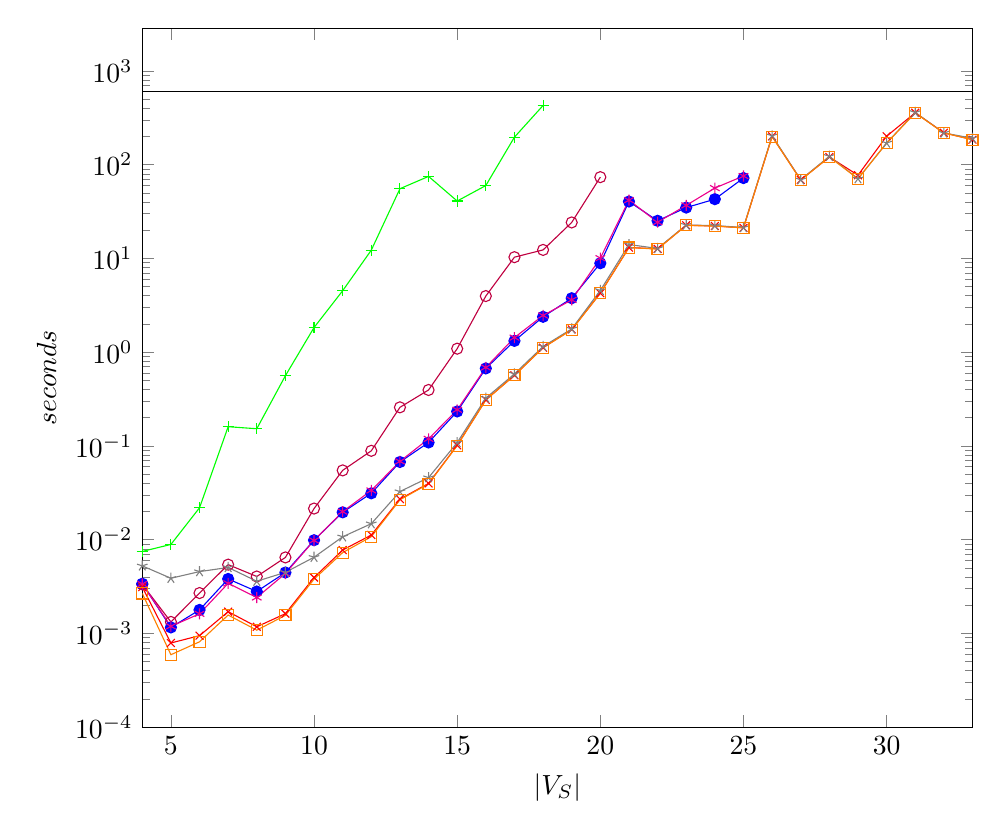
\begin{tikzpicture}
    \begin{axis}[
        xlabel=$|V_S|$,
        ylabel=$seconds$,
        ymin=0.0001,
        ymode=log,
        xmin=4,
        xmax=33,
        legend style={at={(0.9,0.1)},anchor=south east},
        width=\textwidth,
    ]
    
\addplot[
        mark=none,
        black,
    ] plot coordinates {
        (4,600)
        (33,600)
};
 %   \addlegendentry{Timeout 10m} 
    

    
   \addplot[
        mark=o,
        purple,
    ] plot coordinates {
        (4,0.0033354099999999996)
        (5,0.001327198)
        (6,0.0026972415)
        (7,0.005420836)
        (8,0.004050544)
        (9,0.006470579)
        (10,0.021485644)
        (11,0.0548721365)
        (12,0.0887547805)
        (13,0.258150266)
        (14,0.39556562399999995)
        (15,1.0907645185)
        (16,3.971699851282051)
        (17,10.321538780851064)
        (18,12.337433302040818)
        (19,24.217103684000005)
        (20,73.71199097)
};
%    \addlegendentry{GDFS O IP}
    
    
    
    \addplot[
        mark=+,
        green,
    ] plot coordinates {
        (4,0.0074964425000000005)
        (5,0.008899364)
        (6,0.021902257999999997)
        (7,0.160471234)
        (8,0.15263485899999998)
        (9,0.561916418)
        (10,1.833818564)
        (11,4.52718843880597)
        (12,12.26901466122449)
        (13,55.44448909999999)
        (14,75.0789921)
        (15,40.98504065555555)
        (16,59.94558265)
        (17,196.817508975)
        (18,428.4561328)
};
 %   \addlegendentry{CP}
    
    
    \addplot[
        mark=*,
        blue,
    ] plot coordinates {
        (4,0.0033891155)
        (5,0.0011595824999999999)
        (6,0.0017819205)
        (7,0.0038146409999999997)
        (8,0.0028014885)
        (9,0.004467115)
        (10,0.0098760425)
        (11,0.019585361000000003)
        (12,0.031251991)
        (13,0.067427614)
        (14,0.108922384)
        (15,0.233365984)
        (16,0.6713743385)
        (17,1.3210855519999998)
        (18,2.386009026)
        (19,3.765988756140351)
        (20,8.89447237352941)
        (21,40.502501818750005)
        (22,25.221025914285715)
        (23,34.883353815384616)
        (24,42.90160877142857)
        (25,72.07346983333335)
};
%    \addlegendentry{K-Path}
    
    \addplot[
        mark=asterisk,
        magenta,
    ] plot coordinates {
        (4,0.0033671915)
        (5,0.001190538)
        (6,0.0016191069999999998)
        (7,0.0034239325)
        (8,0.0024179585)
        (9,0.0043627885)
        (10,0.009817592)
        (11,0.019897870499999998)
        (12,0.0335268765)
        (13,0.068505526)
        (14,0.1189895675)
        (15,0.2430346145)
        (16,0.6879985279999999)
        (17,1.4320328555000001)
        (18,2.4644637565)
        (19,3.615006598192771)
        (20,10.072892529508197)
        (21,41.85573263125)
        (22,24.362516080952382)
        (23,36.84446636538462)
        (24,56.330943354545454)
        (25,75.77811247500001)
};
%    \addlegendentry{GDFS A IP}
    
    \addplot[
        mark=x,
        red,
    ] plot coordinates {
        (4,0.003124064)
        (5,7.913285000000001E-4)
        (6,9.468475E-4)
        (7,0.0017073364999999998)
        (8,0.0011771495)
        (9,0.0016255140000000002)
        (10,0.0039480825)
        (11,0.0077563585)
        (12,0.0112181135)
        (13,0.027106744)
        (14,0.039854954500000005)
        (15,0.1016730035)
        (16,0.3102863915)
        (17,0.567070922)
        (18,1.1181295875)
        (19,1.7503998269999999)
        (20,4.263310112765957)
        (21,13.087688980434784)
        (22,12.664759238095238)
        (23,22.604950978378376)
        (24,22.215862426666664)
        (25,21.221224975862068)
        (26,200.80231476666665)
        (27,69.01728853)
        (28,120.91195150000003)
        (29,77.2825083)
        (30,201.28251479999994)
        (31,358.3321691)
        (32,219.1503222)
        (33,184.9894481)
};
 %   \addlegendentry{DFS}
    
    \addplot[
        mark=star,
        gray,
    ] plot coordinates {
        (4,0.0052584419999999995)
        (5,0.0038800225)
        (6,0.0045671005)
        (7,0.005054851500000001)
        (8,0.0036043110000000002)
        (9,0.0044851380000000005)
        (10,0.006500158000000001)
        (11,0.010743765999999998)
        (12,0.014813136499999999)
        (13,0.032617665)
        (14,0.045932047000000004)
        (15,0.10862769200000001)
        (16,0.32415647649999996)
        (17,0.586893169)
        (18,1.1500186795)
        (19,1.772846179)
        (20,4.554298787121212)
        (21,14.077475467441861)
        (22,12.78838592857143)
        (23,22.725297256756754)
        (24,22.44824257)
        (25,21.37612426551724)
        (26,203.35969063333334)
        (27,69.08358688)
        (28,123.07605716000003)
        (29,70.88854776666666)
        (30,170.599628675)
        (31,361.26002704999996)
        (32,217.99103095)
        (33,191.6499955)
};
%    \addlegendentry{GDFS C}
    
    \addplot[
        mark=square,
        orange,
    ] plot coordinates {
        (4,0.0026720765000000004)
        (5,5.931255E-4)
        (6,8.145884999999999E-4)
        (7,0.0015716150000000002)
        (8,0.001083881)
        (9,0.0015602699999999999)
        (10,0.0037946819999999997)
        (11,0.0072780025)
        (12,0.010769405999999999)
        (13,0.026622686)
        (14,0.039441741499999995)
        (15,0.1005090725)
        (16,0.3088769205)
        (17,0.5658370635)
        (18,1.114951387)
        (19,1.7321635599999998)
        (20,4.2505378978723405)
        (21,13.068786297826087)
        (22,12.589129547619047)
        (23,22.530537545945947)
        (24,22.130406946666668)
        (25,21.19573636896552)
        (26,199.31648383333334)
        (27,68.44248519)
        (28,120.89257580000003)
        (29,70.80782896666666)
        (30,169.777134475)
        (31,356.8092052)
        (32,217.99103095)
        (33,184.9894481)
};
 %   \addlegendentry{portfolio}

    \end{axis}
    \end{tikzpicture}

\caption{$|V_T|=1\frac{1}{2}|V_S|$}
\label{fig:sub1}
\end{subfigure}%
\begin{subfigure}{.5\linewidth}
\centering

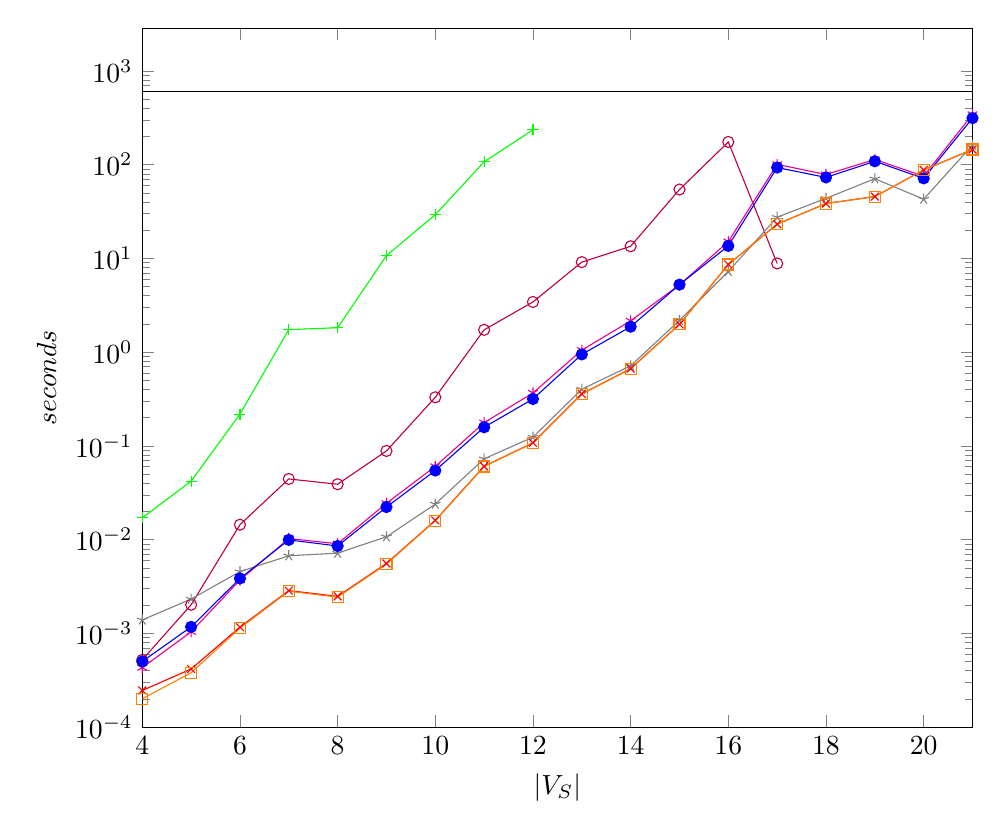
\begin{tikzpicture}
    \begin{axis}[
        xlabel=$|V_S|$,
        ylabel=$seconds$,
        ymin=0.0001,
        ymode=log,
        xmin=4,
        xmax=21,
        legend style={at={(0.9,0.1)},anchor=south east},
        width=\textwidth,
    ]
    
\addplot[
        mark=none,
        black,
    ] plot coordinates {
        (4,600)
        (21,600)
};
 %   \addlegendentry{Timeout 10m} 
    

\addplot[
        mark=+,
        green,
    ] plot coordinates {
        (4,0.017118874)
        (5,0.042044554000000005)
        (6,0.21861366149999997)
        (7,1.7413124975)
        (8,1.824231057)
        (9,10.718911422807018)
        (10,29.285856038095236)
        (11,107.36171433333334)
        (12,235.52224905)
};
%    \addlegendentry{CP}
    
    
    \addplot[
        mark=o,
        purple,
    ] plot coordinates {
        (4,5.229545E-4)
        (5,0.0020221634999999997)
        (6,0.014452913000000001)
        (7,0.044465508)
        (8,0.039038954)
        (9,0.088448429)
        (10,0.33017173499999997)
        (11,1.7330093685)
        (12,3.436815223163842)
        (13,9.139001624999999)
        (14,13.487728657446809)
        (15,54.37308013571429)
        (16,174.90209208000002)
        (17,8.8468752)
};
%    \addlegendentry{GDFS O IP}
    
    \addplot[
        mark=star,
        gray,
    ] plot coordinates {
        (4,0.00139258)
        (5,0.002327794)
        (6,0.004565538)
        (7,0.0067396635000000005)
        (8,0.0071890365)
        (9,0.010737805)
        (10,0.02400474)
        (11,0.07292148550000001)
        (12,0.12421214450000001)
        (13,0.403000701)
        (14,0.7163419985)
        (15,2.1890222930000003)
        (16,7.270705493975904)
        (17,27.538684308695654)
        (18,43.79655899583333)
        (19,70.8624523888889)
        (20,42.929491375)
        (21,161.7936666)
};
 %   \addlegendentry{GDFS C}
    
    \addplot[
        mark=x,
        red,
    ] plot coordinates {
        (4,2.463635E-4)
        (5,4.17268E-4)
        (6,0.001167168)
        (7,0.002865959)
        (8,0.0024855845)
        (9,0.0055816305)
        (10,0.016075872499999998)
        (11,0.060558201)
        (12,0.1081205275)
        (13,0.358527165)
        (14,0.6678748950000001)
        (15,1.9833789535)
        (16,8.623507047058824)
        (17,23.20956361923077)
        (18,38.53969741666666)
        (19,45.70503912307693)
        (20,88.00206148888888)
        (21,145.2799635)
};
%    \addlegendentry{DFS}
    
    
    \addplot[
        mark=asterisk,
        magenta,
    ] plot coordinates {
        (4,4.3166750000000006E-4)
        (5,0.0010404115)
        (6,0.003709151)
        (7,0.010290998499999999)
        (8,0.009050423)
        (9,0.0244776325)
        (10,0.060524060500000004)
        (11,0.177295532)
        (12,0.36728383800000003)
        (13,1.0505953314999998)
        (14,2.158745016)
        (15,5.232621873043478)
        (16,15.130776390697672)
        (17,100.89787280000002)
        (18,78.64249841111112)
        (19,113.64276582222222)
        (20,75.4335271625)
        (21,343.9340747)
};
%    \addlegendentry{GDFS A IP}
    
    \addplot[
        mark=*,
        blue,
    ] plot coordinates {
        (4,5.025650000000001E-4)
        (5,0.0011748805)
        (6,0.0038617564999999998)
        (7,0.009955469500000001)
        (8,0.008569285)
        (9,0.022299932)
        (10,0.054706759)
        (11,0.158324873)
        (12,0.317071005)
        (13,0.9476776635)
        (14,1.870529588)
        (15,5.256302935245901)
        (16,13.612862210869567)
        (17,93.2565386888889)
        (18,73.17322655555556)
        (19,108.78198909999999)
        (20,71.5219922)
        (21,314.1443365)
};
%    \addlegendentry{K-Path}
    
    \addplot[
        mark=square,
        orange,
    ] plot coordinates {
        (4,2.01024E-4)
        (5,3.8098600000000004E-4)
        (6,0.001139124)
        (7,0.0028233219999999996)
        (8,0.00244008)
        (9,0.0054960905)
        (10,0.015953537)
        (11,0.060388840000000006)
        (12,0.107574184)
        (13,0.358221664)
        (14,0.662612554)
        (15,1.9811704315)
        (16,8.621956076470587)
        (17,23.20956361923077)
        (18,38.53969741666666)
        (19,45.70503912307693)
        (20,88.00206148888888)
        (21,145.2799635)
};
 %   \addlegendentry{portfolio}
    

  
    \end{axis}
    \end{tikzpicture}

\caption{$|V_T|=3|V_S|$}
\label{fig:sub2}
\end{subfigure}\\[1ex]
\begin{subfigure}{0.5\linewidth}
\centering

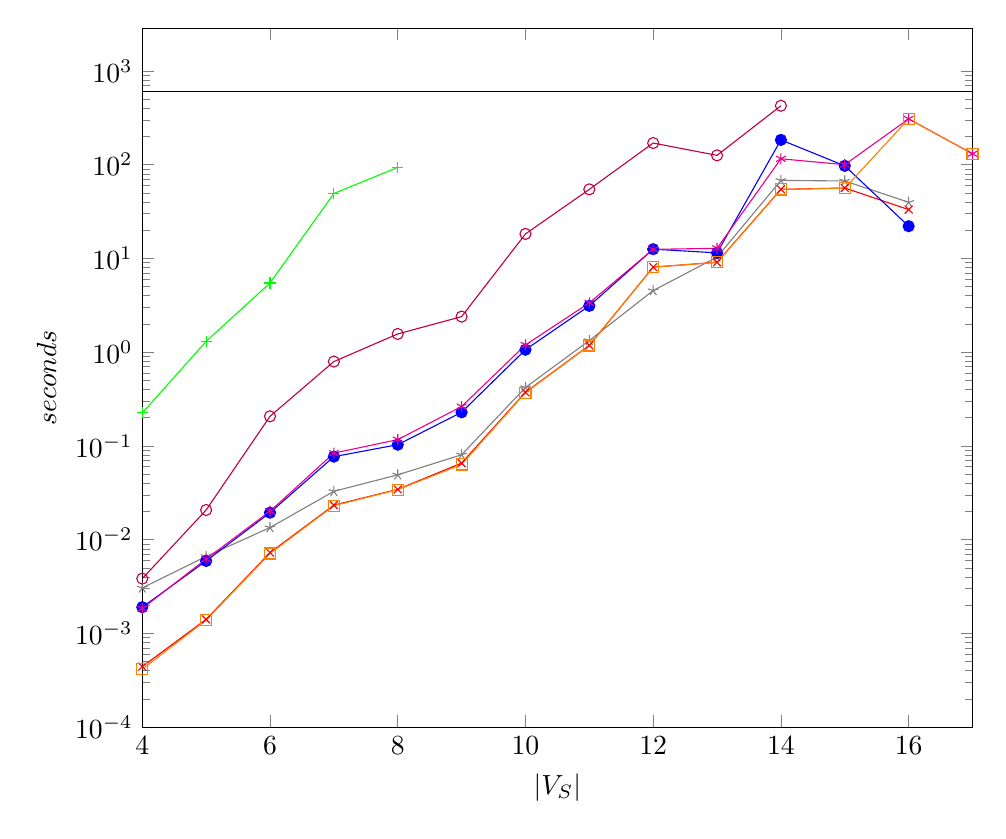
\begin{tikzpicture}
    \begin{axis}[
        xlabel=$|V_S|$,
        ylabel=$seconds$,
        ymin=0.0001,
        ymode=log,
        xmin=4,
        xmax=17,
        legend style={at={(0.9,0.1)},anchor=south east},
        width=\textwidth,
    ]
    
\addplot[
        mark=none,
        black,
    ] plot coordinates {
        (4,600)
        (17,600)
};
 %   \addlegendentry{Timeout 10m} 
    


\addplot[
        mark=+,
        green,
    ] plot coordinates {
        (4,0.22498123849999999)
        (5,1.305544137)
        (6,5.477192146428571)
        (7,49.320910733333335)
        (8,93.62391244)
};
%    \addlegendentry{CP}
    
    
    \addplot[
        mark=star,
        gray,
    ] plot coordinates {
        (4,0.003058187)
        (5,0.0066316019999999995)
        (6,0.013466777000000001)
        (7,0.032822169)
        (8,0.049183345)
        (9,0.080513419)
        (10,0.4200455685)
        (11,1.3332708905000001)
        (12,4.545143440151515)
        (13,10.333796216470589)
        (14,68.03150406)
        (15,67.08428195454545)
        (16,39.747431)
};
%    \addlegendentry{GDFS C}
    
    \addplot[
        mark=x,
        red,
    ] plot coordinates {
        (4,4.4261750000000003E-4)
        (5,0.0014131274999999999)
        (6,0.0072753685000000005)
        (7,0.023372011)
        (8,0.0344219615)
        (9,0.0656533275)
        (10,0.3738274895)
        (11,1.183567724)
        (12,8.084725380597014)
        (13,9.105788104705884)
        (14,54.59190611666667)
        (15,56.45855956363636)
        (16,33.2144619)
};
%    \addlegendentry{DFS}
    
    \addplot[
        mark=*,
        blue,
    ] plot coordinates {
        (4,0.001906137)
        (5,0.005935332)
        (6,0.0194225855)
        (7,0.0768926385)
        (8,0.103136142)
        (9,0.228699563)
        (10,1.062870499)
        (11,3.1228105518134712)
        (12,12.555450586)
        (13,11.474581472222223)
        (14,183.9983442333333)
        (15,97.27099918571427)
        (16,22.0919737)
};
%    \addlegendentry{K-Path}
    
    
    \addplot[
        mark=o,
        purple,
    ] plot coordinates {
        (4,0.0038459365)
        (5,0.020740273)
        (6,0.20711417999999998)
        (7,0.7947821999999999)
        (8,1.565915889)
        (9,2.396293172)
        (10,18.270429463636365)
        (11,54.59309324615385)
        (12,170.3045068)
        (13,125.79853659999999)
        (14,425.516946)
};
%    \addlegendentry{GDFS O IP}
    
    
    \addplot[
        mark=asterisk,
        magenta,
    ] plot coordinates {
        (4,0.0018444635000000001)
        (5,0.006224887500000001)
        (6,0.0201156265)
        (7,0.0838507)
        (8,0.11677660100000001)
        (9,0.2631939955)
        (10,1.195823311)
        (11,3.358671161111111)
        (12,12.508858883333334)
        (13,12.832528379245282)
        (14,115.64856344)
        (15,100.09827916666666)
        (16,308.21460745)
        (17,130.7677965)
};
%    \addlegendentry{GDFS A IP}
    
    
    \addplot[
        mark=square,
        orange,
    ] plot coordinates {
        (4,4.152115E-4)
        (5,0.001389112)
        (6,0.0071271165)
        (7,0.023055476000000002)
        (8,0.034188356)
        (9,0.0634472525)
        (10,0.370240898)
        (11,1.1794381704999999)
        (12,8.077388874626866)
        (13,9.088254795294118)
        (14,54.45241678333334)
        (15,56.29606548181818)
        (16,308.21460745)
        (17,130.7677965)
};
%    \addlegendentry{portfolio}
    
  
    \end{axis}
    \end{tikzpicture}

\caption{$|V_T|=5|V_S|$}
\label{fig:sub3}
\end{subfigure}
\begin{subfigure} {0.5\linewidth}
\centering

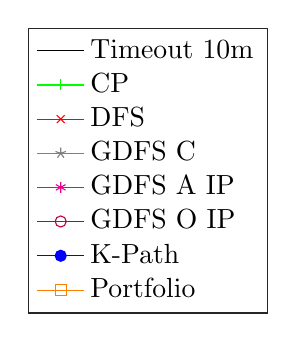
\begin{tikzpicture} 
    \begin{axis}[%
    hide axis,
    xmin=10,
    xmax=50,
    ymin=0,
    ymax=0.4,
    legend style={draw=white!15!black,legend cell align=left}
    ]
	\addlegendimage{black}
    \addlegendentry{Timeout 10m}; 
     
    \addlegendimage{green, mark=+}
    \addlegendentry{CP};
    
    \addlegendimage{red, mark=x}
    \addlegendentry{DFS};
    
    \addlegendimage{gray, mark=star}
    \addlegendentry{GDFS C};
    
    \addlegendimage{magenta, mark=asterisk}
    \addlegendentry{GDFS A IP};
    
    \addlegendimage{purple, mark=o}
    \addlegendentry{GDFS O IP};
    
    \addlegendimage{blue, mark=*}
    \addlegendentry{K-Path};
    
    \addlegendimage{orange, mark=square}
    \addlegendentry{Portfolio};
    \end{axis}
\end{tikzpicture}

\end{subfigure}

\caption{Performance of using different path iterators in test cases with present subgraph homeomorphisms. We include a portfolio method that takes the best performance rating for each individual test case.}	
\label{fig:test}
\end{figure}




%\centering
%\begin{tikzpicture}
%    \begin{axis}[
%        xlabel=$|V_S|$,
%        ylabel=$seconds$,
%        ymin=0.0001,
%        ymode=log,
%        xmin=4,
%        xmax=154,
%        legend style={at={(0.9,0.1)},anchor=south east},
%        width=\textwidth,
%    ]
%    
%    
%    \addplot[
%        mark=*,
%        blue,
%    ] plot coordinates {
%        (4,0.001453558)
%        (5,2.662845E-4)
%        (6,2.692255E-4)
%        (7,2.766865E-4)
%        (8,2.85301E-4)
%        (9,2.95161E-4)
%        (10,2.62594E-4)
%        (11,3.120675E-4)
%        (12,3.0024450000000003E-4)
%        (13,3.8988799999999996E-4)
%        (14,3.98057E-4)
%        (15,4.38608E-4)
%        (16,5.407825E-4)
%        (17,4.2873550000000003E-4)
%        (18,4.97956E-4)
%        (19,5.5585E-4)
%        (20,5.752355E-4)
%        (21,7.143774999999999E-4)
%        (22,6.579855E-4)
%        (23,7.275845E-4)
%        (24,7.86211E-4)
%        (25,8.5834E-4)
%        (26,9.02515E-4)
%        (27,9.85177E-4)
%        (28,0.001070911)
%        (29,0.0011007185)
%        (30,0.0011748260000000001)
%        (31,0.0013961960000000002)
%        (32,0.001337548)
%        (33,0.0015390924999999999)
%        (34,0.001610745)
%        (35,0.001603441)
%        (36,0.0017608695)
%        (37,0.0018374584999999999)
%        (38,0.0019971715)
%        (39,0.001988867)
%        (40,0.0021071205000000003)
%        (41,0.002299212)
%        (42,0.0023479385)
%        (43,0.0025216235)
%        (44,0.0026287565)
%        (45,0.0027482985)
%        (46,0.0029241840000000002)
%        (47,0.0030328865)
%        (48,0.003001125)
%        (49,0.0033098305)
%        (50,0.00341402)
%        (51,0.003456682)
%        (52,0.0035689510000000003)
%        (53,0.003724974)
%        (54,0.003964841)
%        (55,0.004148001)
%        (56,0.0041462395)
%        (57,0.004439741)
%        (58,0.004803864)
%        (59,0.0047600494999999994)
%        (60,0.004885047)
%        (61,0.0051423625)
%        (62,0.005801905)
%        (63,0.0058080555)
%        (64,0.005837875)
%        (65,0.0060842629999999995)
%        (66,0.0058939644999999995)
%        (67,0.006689764999999999)
%        (68,0.006344105)
%        (69,0.006680382499999999)
%        (70,0.006976954)
%        (71,0.007048449500000001)
%        (72,0.006898754)
%        (73,0.0075829124999999995)
%        (74,0.007442074)
%        (75,0.0077876275)
%        (76,0.008074942)
%        (77,0.0080991655)
%        (78,0.008379599)
%        (79,0.00874456)
%        (80,0.008639861)
%        (81,0.009265389)
%        (82,0.009434129)
%        (83,0.009594110500000001)
%        (84,0.009608555)
%        (85,0.009872137)
%        (86,0.010385803499999999)
%        (87,0.01062902)
%        (88,0.0108560975)
%        (89,0.010737672)
%        (90,0.011210833)
%        (91,0.0118001685)
%        (92,0.01171153)
%        (93,0.012064637)
%        (94,0.0123413575)
%        (95,0.012456216499999999)
%        (96,0.013313942)
%        (97,0.013196973)
%        (98,0.013713651)
%        (99,0.013467091499999998)
%        (100,0.0140739155)
%        (101,0.0145949875)
%        (102,0.0147315415)
%        (103,0.015095879999999999)
%        (104,0.014955354999999998)
%        (105,0.015345967)
%        (106,0.016499721000000002)
%        (107,0.016180731)
%        (108,0.0165881175)
%        (109,0.017206793)
%        (110,0.017553430999999998)
%        (111,0.0178276065)
%        (112,0.01793235)
%        (113,0.0185217045)
%        (114,0.019131549)
%        (115,0.0193583435)
%        (116,0.0194724465)
%        (117,0.0200064025)
%        (118,0.0205588975)
%        (119,0.020825203499999997)
%        (120,0.021444926)
%        (121,0.022597493000000003)
%        (122,0.025429853)
%        (123,0.024438607)
%        (124,0.023428064000000002)
%        (125,0.023900668500000003)
%        (126,0.025059102000000003)
%        (127,0.025008305)
%        (128,0.0251174765)
%        (129,0.025973405)
%        (130,0.027299354)
%        (131,0.028161115)
%        (132,0.027549519999999997)
%        (133,0.0283001935)
%        (134,0.0282419815)
%        (135,0.029244735)
%        (136,0.028565097)
%        (137,0.0299900245)
%        (138,0.032137683)
%        (139,0.03258433103448276)
%        (140,0.0309644735)
%        (141,0.032145942999999996)
%        (142,0.032131891499999995)
%        (143,0.03353229593495935)
%        (144,0.032666537704918036)
%        (145,0.03342298187134503)
%        (146,0.033846469)
%        (147,0.034949912068965514)
%        (148,0.03325529607843137)
%        (149,0.03422327)
%        (150,0.03498731012658228)
%        (151,0.036564767724867726)
%        (152,0.0382647295)
%        (153,0.03801780508474576)
%        (154,0.038082844)
%};
%    \addlegendentry{K-Path}
%    
%   
%  
%    \end{axis}
%    \end{tikzpicture}
%    \caption{Time spent where}
%    \label{fig:plotfailiterators}
%\end{figure}





%time to succeed \ref{fig:plotsucceediterators} TODO: run 10m each
%\begin{figure}
%\centering
%\begin{tikzpicture}
%    \begin{axis}[
%        xlabel=$|V_S|$,
%        ylabel=$seconds$,
%        ymin=0.01,
%        ymode=log,
%        xmin=4,
%        xmax=21,
%        legend style={at={(0.9,0.1)},anchor=south east},
%        width=\textwidth,
%    ]
%    
%    \addplot[
%        mark=none,
%        black,
%    ] plot coordinates {
%        (4,600)
%        (21,600)
%};
%    \addlegendentry{Timeout 10m}
%
%
%\addplot[
%        mark=*,
%        blue,
%        error bars/.cd, y dir=both, y explicit,
%    ] plot coordinates {
%        (4,0.0012667032822330576)
%        (5,0.014450939583729977)
%        (6,0.05591708867636635)
%        (7,0.14911566497364495)
%        (8,0.44854427304185357)
%        (9,1.257458328264463)
%        (10,4.882261796422765)
%        (11,8.92112126069014)
%        (12,53.879064942750006)
%        (13,50.1927055715)
%};
%    \addlegendentry{K-Path}
%    
%    \addplot[
%        mark=+,
%        green,
%        error bars/.cd, y dir=both, y explicit,
%    ] plot coordinates {
%        (4,0.0022598064731390965)
%        (5,0.040788492474074574)
%        (6,0.18285989427787933)
%        (7,0.7438714740483271)
%        (8,2.0661439080927835)
%        (9,11.051631589785714)
%        (10,26.467970115956522)
%        (11,91.75283437071428)
%        (12,114.154734211)
%        (13,342.4216391745)
%};
%    \addlegendentry{CP}
%    
%    
%    \addplot[
%        mark=o,
%        purple,
%        error bars/.cd, y dir=both, y explicit,
%    ] plot coordinates {
%        (4,7.913821003220384E-4)
%        (5,0.008231382983722117)
%        (6,0.031882214566006595)
%        (7,0.08963993490432053)
%        (8,0.29087998969535783)
%        (9,0.6738117268754134)
%        (10,1.8639315102639753)
%        (11,4.723388754421875)
%        (12,19.076032830888888)
%        (13,34.09402854616666)
%        (14,56.448447976636366)
%        (15,221.585912108)
%        (16,271.705023368)
%};
%    \addlegendentry{GDFS O IP}
%    
%    
%    \addplot[
%        mark=x,
%        red,
%        error bars/.cd, y dir=both, y explicit,
%    ] plot coordinates {
%        (4,5.262049048412901E-4)
%        (5,0.0037078367276320813)
%        (6,0.011864989818313664)
%        (7,0.024878632873617693)
%        (8,0.06746086448666291)
%        (9,0.1434635451083732)
%        (10,0.42305252119181946)
%        (11,0.8507154702662889)
%        (12,2.2694573458389513)
%        (13,4.062910206266234)
%        (14,15.418462455714286)
%        (15,88.48300721233333)
%};
%    \addlegendentry{DFS}
%    
%    
%    \addplot[
%        mark=asterisk,
%        black,
%        error bars/.cd, y dir=both, y explicit,
%    ] plot coordinates {
%        (4,0.0012375753780820582)
%        (5,0.01386437069184402)
%        (6,0.053590561273019845)
%        (7,0.1357242449547409)
%        (8,0.3913462516747066)
%        (9,0.9992033137657806)
%        (10,2.177200933823741)
%        (11,5.359800497321429)
%        (12,14.644324665268291)
%        (13,39.5231686368125)
%        (14,127.138527012)
%        (15,40.69748180766667)
%        (16,477.083996688)
%};
%    \addlegendentry{GDFS A IP}
%    
%    
%    \addplot[
%        mark=star,
%        gray,
%        error bars/.cd, y dir=both, y explicit,
%    ] plot coordinates {
%        (4,0.005644702207616498)
%        (5,0.008692270720925143)
%        (6,0.017174057391094375)
%        (7,0.03073833753675828)
%        (8,0.07604849509162437)
%        (9,0.13615389069436876) 
%        (10,0.38220422819426747)
%        (11,0.6959524782169374)
%        (12,1.95247773692233)
%        (13,6.06748104474) 
%        (14,9.499085503648649) 
%        (15,17.829571026735294) 
%        (16,59.15707016833334) 
%        (17,39.30442401336364) 
%        (18,77.68409019719999) 
%        (19,85.162749429) 
%        (20,223.46494652625)
%        (21,113.76846415325) 
%};
%    \addlegendentry{GDFS C}
%
%
%   
%    \end{axis}
%    \end{tikzpicture}
%    \caption{A comparison of the speed of path iterators on directed graphs with a vertex disjoint subgraph homeomorphism. The time taken is measured of exploring the entire search tree without pruning or contraction and ``refuse longer paths" enabled. The source graph has average degree $3.0$ and the random target graph has $50\%$ more vertices and average degree $4.0$.}
%    \label{fig:plotsucceediterators}
%\end{figure}



%contraction times factor 1.5 timeout 10m
%\begin{figure}
%\centering
%\begin{tikzpicture}
%    \begin{axis}[
%        xlabel=$|V_S|$,
%        ylabel=$seconds$,
%        ymin=-100,
%        ymax=100,
%        xmin=4,
%        xmax=35,
%        legend style={at={(0.9,0.1)},anchor=south east},
%        width=\textwidth,
%        yticklabel={$\pgfmathprintnumber{\tick}\%$},
%    ]
%
%
%\addplot [mark=none, black] plot coordinates {
%        (4,0) (35, 0)};
%\addlegendentry{No contraction}
%
%
%\addplot[
%        mark=o,
%        purple,
%    ] plot coordinates {
%        (4,123.73282219151496)
%        (5,-15.920345499984956)
%        (6,-52.37305659134008)
%        (7,-65.61004822968585)
%        (8,-65.7340938280165)
%        (9,-25.285589142891307)
%        (10,-68.62051421832805)
%        (11,-80.95502536287958)
%        (12,-73.99134383576952)
%        (13,-80.98147897767203)
%        (14,-73.55201926260625)
%        (15,-78.95355041753565)
%        (16,-81.53448492043376)
%        (17,-86.511466028791)
%        (18,-66.52994544259807)
%        (19,-58.72920400909036)
%        (20,-47.039151254147216)
%        (21,-84.1600528625449)
%        (22,-71.09729745327353)
%        (23,-82.17729995308483)
%};
%    \addlegendentry{GDFS O IP}
%  
%
%
%\addplot[
%        mark=+,
%        green,
%    ] plot coordinates {
%        (4,-025.20219056936399)
%        (5,-022.493453420382936)
%        (6,-038.97463954937388)
%        (7,-055.09778357966048)
%        (8,-037.433492126378953)
%        (9,-032.03325141432528)
%        (10,-051.96689139278652)
%        (11,-057.14050109835533)
%        (12,-058.75023937798425)
%        (13,-047.140986025169374)
%        (14,-090.23397911753834)
%        (15,239.8585596188363)
%        (16,-049.057976977453943)
%        (17,-098.51586058140065)
%};
%    \addlegendentry{CP}
%    
%    
%    \addplot[
%        mark=asterisk,
%        yellow,
%    ] plot coordinates {
%        (4,104.32230154808875)
%        (5,001.3100718127611488)
%        (6,-012.62414524078096)
%        (7,-037.8202125606379)
%        (8,-024.350567006027835)
%        (9,003.142150672347355)
%        (10,-039.07757134579495)
%        (11,-048.82593836023965)
%        (12,-044.182147606506306)
%        (13,-053.61037313840382)
%        (14,-056.59671859613651)
%        (15,-049.744416960439364)
%        (16,-048.44972253467088)
%        (17,-054.58078239119416)
%        (18,-033.656157042382806)
%        (19,-028.379096681296656)
%        (20,-034.283862074351223)
%        (21,-059.59967793745939)
%        (22,-001.798229780964855)
%        (23,-092.35029400370509)
%        (24,-086.31485796364881)
%        (25,-067.74926355062878)
%        (26,-094.84247146483261)
%        (27,-097.99256891572952)
%        (28,-096.97865670660217)
%        (29,-016.044463767008554)
%        (30,-053.54445552007417)
%        (31,-097.25503699400231)
%};
%    \addlegendentry{GDFS A IP}
%    
%    
%    \addplot[
%        mark=*,
%        blue,
%    ] plot coordinates {
%        (4,168.43679566347465)
%        (5,026.442489966216587)
%        (6,-002.225130638006434)
%        (7,-025.153452900976225)
%        (8,-015.497750469129457)
%        (9,017.423429164778614)
%        (10,-026.24191043443711)
%        (11,-032.430479287090885)
%        (12,-021.048904390943224)
%        (13,-038.76743561292725)
%        (14,-045.36566245712572)
%        (15,-028.920176244755447)
%        (16,-030.40272084329029)
%        (17,-033.608990208004486)
%        (18,-009.674324307431459)
%        (19,003.924445129779297)
%        (20,-016.033797858120757)
%        (21,-052.22128629074319)
%        (22,024.260726237431385)
%        (23,-090.45931913063434)
%        (24,-084.34122719202735)
%        (25,-051.94077123219644)
%        (26,-094.08535824980668)
%        (27,-097.92626199110588)
%        (28,-095.96588266125698)
%        (29,-046.47193982745663)
%        (30,-044.42559644925941)
%        (31,-097.18674546373528)
%};
%    \addlegendentry{K-Path}
%    
%    
%    \addplot[
%        mark=x,
%        red,
%    ] plot coordinates {
%        (4,145.74288201398948)
%        (5,023.590100009510784)
%        (6,020.559035149385996)
%        (7,010.006338541144788)
%        (8,051.3310950749601)
%        (9,130.73410526666702)
%        (10,006.359679066853641)
%        (11,-015.70413117521775)
%        (12,-005.93144906987042)
%        (13,-034.452080777339855)
%        (14,-037.4983499537888)
%        (15,-024.78591933478047)
%        (16,-036.156546968784553)
%        (17,-028.39745050978739)
%        (18,-023.36065635058614)
%        (19,-015.643925874671583)
%        (20,-043.99928871595725)
%        (21,-061.33973110766648)
%        (22,022.841018680086767)
%        (23,-091.35376669657393)
%        (24,-079.92603408025085)
%        (25,-046.120410300036896)
%        (26,-091.27231419272499)
%        (27,-096.07259933786477)
%        (28,-083.75935288922367)
%        (29,158.9756916506027)
%        (30,-057.69659226493207)
%        (31,-098.51434243131209)
%        (32,-099.94784335719136)
%        (33,-051.02543885749924)
%        (34,-025.99547070749336)
%};
%    \addlegendentry{DFS}
%    
%    
%    \addplot[
%        mark=star,
%        gray,
%    ] plot coordinates {
%        (4,239.941105252917)
%        (5,071.15229717186846)
%        (6,036.730285185821154)
%        (7,006.1613749961845654)
%        (8,003.793627194674065)
%        (9,016.909679152992885)
%        (10,-010.53244807095538)
%        (11,-030.898248312359733)
%        (12,-028.582837812180484)
%        (13,-049.40914532675378)
%        (14,-050.81645782291583)
%        (15,-053.2318090474718)
%        (16,-060.45571353433861)
%        (17,-057.22988218928096)
%        (18,-053.53324295775679)
%        (19,-046.71770062217261)
%        (20,-064.09412074839498)
%        (21,-067.93950642114399)
%        (22,-017.747465972450327)
%        (23,-096.15557392514883)
%        (24,-077.18833763705579)
%        (25,-066.20231377739343)
%        (26,-095.28781711900244)
%        (27,-097.54987368150285)
%        (28,-093.96006304153799)
%        (29,-059.83758603184788)
%        (30,-061.25671690568346)
%        (31,-098.33086459795161)
%        (32,-099.9913245774606)
%        (33,-079.02405113835651)
%        (34,-063.69394803292339)
%        (35,1943.520257459911)
%};
%    \addlegendentry{GDFS C}
%    
%    
%    \addplot[
%        mark=square,
%        orange,
%    ] plot coordinates {
%        (4,-035.18057819844859)
%        (5,-039.07625593738285)
%        (6,-045.56962725740414)
%        (7,-060.65228722082426)
%        (8,-063.1323457667123)
%        (9,-060.7256583365869)
%        (10,-070.19172476203214)
%        (11,-067.39249160120488)
%        (12,-064.17656627335265)
%        (13,-072.45468048165767)
%        (14,-065.09256151173232)
%        (15,-070.35172278405152)
%        (16,-070.34365027550014)
%        (17,-059.50201450871458)
%        (18,-065.21704112562756)
%        (19,-064.41343850179483)
%        (20,-060.00235109601747)
%        (21,-057.59166958306023)
%        (22,-034.158096253727355)
%        (23,-077.52213868588044)
%        (24,-080.41428261543347)
%        (25,-073.93216920275777)
%        (26,-082.62941996091215)
%        (27,-098.46321740243816)
%        (28,-078.42040881354694)
%        (29,-059.83758603184788)
%        (30,-062.08337850557739)
%        (31,-073.59160791446231)
%        (32,-099.9913245774606)
%        (33,-079.43456610669396)
%        (34,-042.56917398865643)
%        (35,0.0)
%};
%    \addlegendentry{portfolio}
%
%
%    \end{axis}
%    \end{tikzpicture}
%    \caption{Relative time consumption of contraction-enabled subgraph homeomorphism search compared to contraction-disabled for different path iteration methods.}
%    \label{fig:contractionsmall}
%\end{figure}


%contraction times factor 1.5 timeout 30m
\begin{figure}
\centering

    \caption{Mean relative time consumption of contraction-enabled subgraph homeomorphism search compared to contraction-disabled for different path iteration methods. For data points below the reference line contraction saves time while for data points above it contraction costs extra time. We handled a maximum of 1000 test cases or 30 minutes per value of $|V_S|$ for each path iteration method.}
    \label{fig:contractionsmall}
\end{figure}








\begin{figure}
\begin{subfigure}{.5\linewidth}
\centering

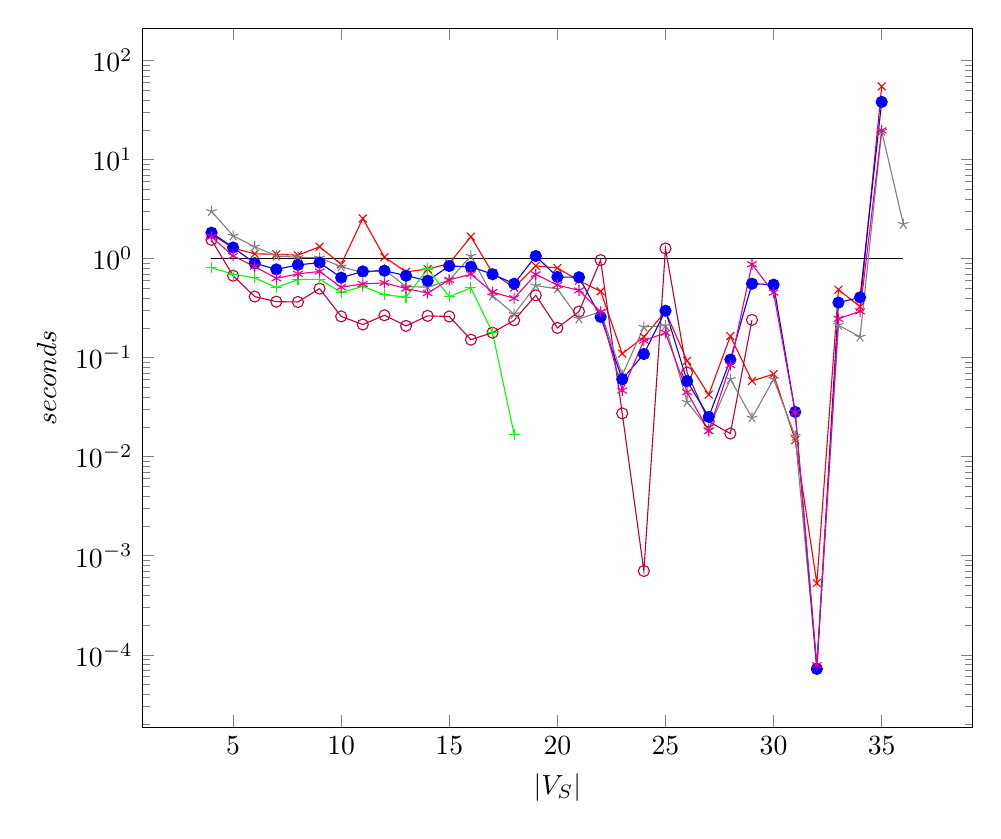
\begin{tikzpicture}
    \begin{axis}[
        xlabel=$|V_S|$,
        ylabel=$seconds$,
        ymode=log,
        legend style={at={(0.9,0.1)},anchor=south east},
        width=\textwidth,
		y tick label style={/pgf/number format/sci},
    ]


\addplot [mark=none, black] plot coordinates {
        (4,1) (36, 1)};
%\addlegendentry{No contraction}

	
    \addplot[
        mark=x,
        red,
    ] plot coordinates {
        (4,1.764570104072358)
        (5,1.2804472403537654)
        (6,1.1184611822085426)
        (7,1.108193754987779)
        (8,1.0823455102636332)
        (9,1.3202304844536292)
        (10,0.8766301350767352)
        (11,2.545919815002013)
        (12,1.0352805568707166)
        (13,0.7348584756068407)
        (14,0.7849914287368015)
        (15,0.8934474568976407)
        (16,1.6666025961560895)
        (17,0.71724791351521)
        (18,0.5094398225741126)
        (19,0.8456597164761079)
        (20,0.8045735438552715)
        (21,0.5994679253970462)
        (22,0.4676165222586781)
        (23,0.10986432258137258)
        (24,0.16189794326161777)
        (25,0.2926263173443996)
        (26,0.09304326805518515)
        (27,0.042335345258718515)
        (28,0.1650463503335008)
        (29,0.05828381864786569)
        (30,0.06816890123257702)
        (31,0.014702001658170927)
        (32,5.292125517369906E-4)
        (33,0.48658861405918064)
        (34,0.3275583732734606)
        (35,54.77402524625391)
};
%    \addlegendentry{DFS}



\addplot[
        mark=o,
        purple,
    ] plot coordinates {
        (4,1.5465954055848148)
        (5,0.6725582833953612)
        (6,0.4139609581308408)
        (7,0.36803303109353136)
        (8,0.36527194171296373)
        (9,0.49852548813528896)
        (10,0.26095750210484203)
        (11,0.21624262398197047)
        (12,0.26820633077466083)
        (13,0.20928330156141128)
        (14,0.26458447534228824)
        (15,0.2606750959815698)
        (16,0.1519838230882713)
        (17,0.17898927491143424)
        (18,0.2388521888406996)
        (19,0.4267188749902131)
        (20,0.19982250009097213)
        (21,0.2924664720196809)
        (22,0.9672401778006531)
        (23,0.027360410960048376)
        (24,7.01509756650176E-4)
        (25,1.2672226912043596)
        (26,0.07078753406996308)
        (27,0.022665056711590914)
        (28,0.017141291453382168)
        (29,0.24055888434774642)
};
%    \addlegendentry{GDFS O IP}


    \addplot[
        mark=star,
        gray,
    ] plot coordinates {
        (4,3.0103172170217087)
        (5,1.7008010826730877)
        (6,1.3185993107748495)
        (7,1.0651222844937673)
        (8,1.0313582598355582)
        (9,1.019847433896466)
        (10,0.8297884970625686)
        (11,0.7200492247409158)
        (12,0.774512334885343)
        (13,0.5217949486742455)
        (14,0.5149663295021711)
        (15,0.6077016349543982)
        (16,1.0645804487651895)
        (17,0.4211041381764984)
        (18,0.2746875518186591)
        (19,0.5346278517377602)
        (20,0.4954917433705648)
        (21,0.24700068708986667)
        (22,0.2909598485628878)
        (23,0.06682556779896554)
        (24,0.20424256710140876)
        (25,0.2106670647954565)
        (26,0.035665701539059236)
        (27,0.018999300275658104)
        (28,0.06081303305299257)
        (29,0.02467804462419776)
        (30,0.06069641418283933)
        (31,0.016093817467386362)
        (32,7.397912089912584E-5)
        (33,0.21324629155751507)
        (34,0.1619915480935199)
        (35,19.49048948725945)
        (36,2.2331192579992156)
};
%    \addlegendentry{GDFS C}

    \addplot[
        mark=*,
        blue,
    ] plot coordinates {
        (4,1.8288452494372274)
        (5,1.296842120241007)
        (6,0.9012387818727957)
        (7,0.7791122372023914)
        (8,0.864968223092994)
        (9,0.911626513812194)
        (10,0.6427888393538057)
        (11,0.7436225584218299)
        (12,0.7549604979371962)
        (13,0.6725293793784693)
        (14,0.5992914625619475)
        (15,0.8435469822917079)
        (16,0.8272824596684006)
        (17,0.6960713562008894)
        (18,0.558150986832071)
        (19,1.0626322277949884)
        (20,0.6533296061774068)
        (21,0.6487638110734476)
        (22,0.2578033809500446)
        (23,0.06052594706960124)
        (24,0.10891268807752708)
        (25,0.2980748961720695)
        (26,0.05796008903103311)
        (27,0.025237959619589523)
        (28,0.09548260902564809)
        (29,0.5586781624508028)
        (30,0.5460070481456223)
        (31,0.02831601533804662)
        (32,7.199585374040307E-5)
        (33,0.3599020863720135)
        (34,0.40664654347704143)
        (35,38.25888474739304)
};
%    \addlegendentry{K-Path}
	\addplot[
        mark=+,
        green,
    ] plot coordinates {
        (4,0.8097147281048784)
        (5,0.6974807076483973)
        (6,0.6387765511195216)
        (7,0.5108136511953608)
        (8,0.6154822873000718)
        (9,0.6178076238665242)
        (10,0.4566675480771135)
        (11,0.5245224457353261)
        (12,0.43193355168311)
        (13,0.4090918564605406)
        (14,0.7867273649511707)
        (15,0.4132124817740861)
        (16,0.506998908675651)
        (17,0.17851266569571234)
        (18,0.016853231440474126)
};
%    \addlegendentry{CP}


    \addplot[
        mark=asterisk,
        magenta,
    ] plot coordinates {
        (4,1.6604963959561405)
        (5,1.0651196386902062)
        (6,0.8313893618484981)
        (7,0.6330831569415312)
        (8,0.7025851289861612)
        (9,0.7421127604924067)
        (10,0.5145838783545251)
        (11,0.555358976224104)
        (12,0.5695323766025293)
        (13,0.4990355735260106)
        (14,0.448887395328494)
        (15,0.6109556736209575)
        (16,0.6965392752667293)
        (17,0.4587395343719304)
        (18,0.3984597147505228)
        (19,0.6943628794563819)
        (20,0.5416331210064403)
        (21,0.47775841013253695)
        (22,0.29035493491769016)
        (23,0.04652391751293539)
        (24,0.14871288585077824)
        (25,0.1781947274150446)
        (26,0.04490122252456785)
        (27,0.018161498301854984)
        (28,0.08401938735395065)
        (29,0.8775983409797485)
        (30,0.4542658231858391)
        (31,0.027895820423659345)
        (32,7.878042538378427E-5)
        (33,0.2469129572361528)
        (34,0.2944533235188781)
        (35,19.738338899024424)
};
%    \addlegendentry{GDFS A IP}

    
   

    \end{axis}
    \end{tikzpicture}


\caption{$|V_T|=1\frac{1}{2}|V_S|$}
\label{fig:sub1}
\end{subfigure}%
\begin{subfigure}{.5\linewidth}
\centering

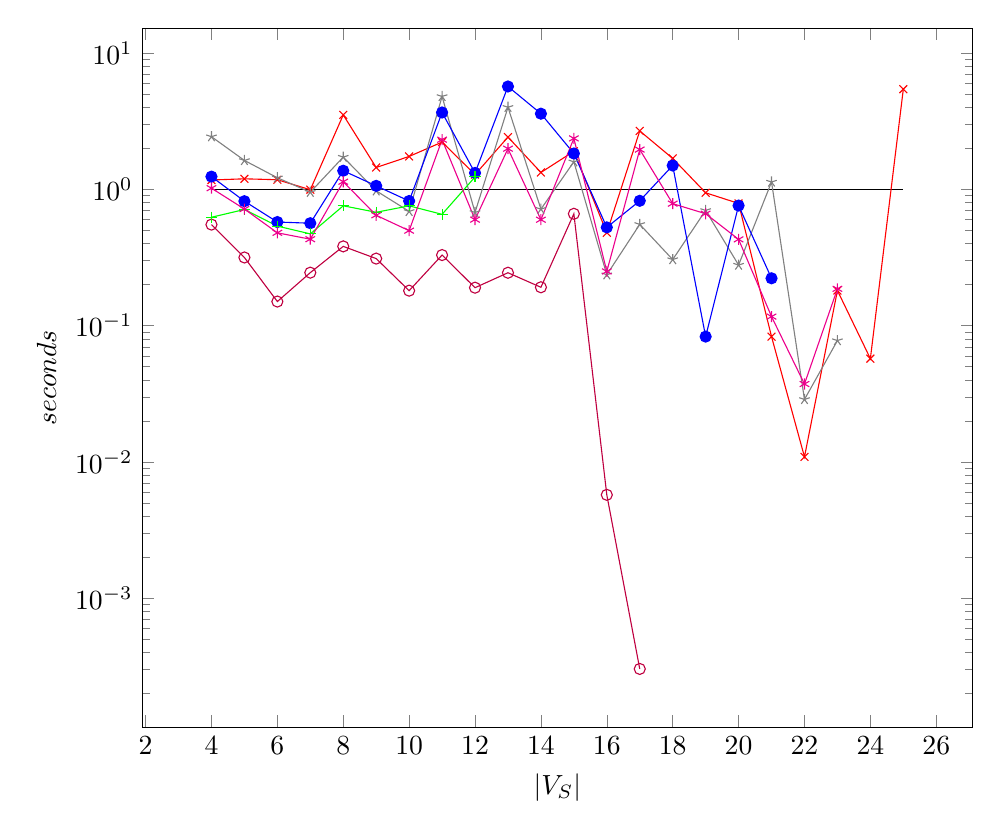
\begin{tikzpicture}
    \begin{axis}[
        xlabel=$|V_S|$,
        ylabel=$seconds$,
        ymode=log,
        legend style={at={(0.9,0.1)},anchor=south east},
        width=\textwidth,
		y tick label style={/pgf/number format/sci},
    ]


\addplot [mark=none, black] plot coordinates {
        (4,1) (25, 1)};
%\addlegendentry{No contraction}

	


\addplot[
        mark=x,
        red,
    ] plot coordinates {
        (4,1.1732605514536567)
        (5,1.196916188570318)
        (6,1.1785456812485087)
        (7,0.9954870013054639)
        (8,3.525437510655584)
        (9,1.4492110968852605)
        (10,1.747381055099775)
        (11,2.2270690506062127)
        (12,1.2853934585525963)
        (13,2.4238390071533145)
        (14,1.3323905497689534)
        (15,1.9053869795283003)
        (16,0.48107044214796724)
        (17,2.689105479333416)
        (18,1.6898544382126748)
        (19,0.9452484856043308)
        (20,0.7898504601171549)
        (21,0.08308472050964744)
        (22,0.010893076925442502)
        (23,0.1812527204673673)
        (24,0.05728059082927839)
        (25,5.443902225728544)
};
%    \addlegendentry{DFS}


\addplot[
        mark=o,
        purple,
    ] plot coordinates {
        (4,0.5520630930461605)
        (5,0.3167780166100581)
        (6,0.15039692039595431)
        (7,0.24510767406414147)
        (8,0.38213533186187054)
        (9,0.3108804215985045)
        (10,0.1807787773743944)
        (11,0.3299920410160406)
        (12,0.19012573181575232)
        (13,0.24472040784270033)
        (14,0.19143954341561553)
        (15,0.6627219343829152)
        (16,0.005733506512017317)
        (17,3.023867931706281E-4)
};
%    \addlegendentry{GDFS O IP}


\addplot[
        mark=star,
        gray,
    ] plot coordinates {
        (4,2.4400816563321017)
        (5,1.633197217665063)
        (6,1.2185290307235452)
        (7,0.9546648292258212)
        (8,1.728111058353678)
        (9,0.9769781523573012)
        (10,0.6904942121852058)
        (11,4.816564314417738)
        (12,0.6783371965634181)
        (13,4.011191995338261)
        (14,0.7170173730516766)
        (15,1.5965119303548203)
        (16,0.23663227697171496)
        (17,0.5542490660149222)
        (18,0.3058591166536577)
        (19,0.7018097729480665)
        (20,0.27875622792926213)
        (21,1.1344734954273632)
        (22,0.028755331201753886)
        (23,0.0777791424367319)
};
%    \addlegendentry{GDFS C}


\addplot[
        mark=*,
        blue,
    ] plot coordinates {
        (4,1.2419213216803755)
        (5,0.8200821368474451)
        (6,0.5765214516413038)
        (7,0.565346845113148)
        (8,1.3724712483006076)
        (9,1.0626551826303774)
        (10,0.8227740807006784)
        (11,3.6735922630894127)
        (12,1.3221239755232121)
        (13,5.700758822957509)
        (14,3.5989514748969498)
        (15,1.8366783161451987)
        (16,0.5267585376114875)
        (17,0.8256958007787268)
        (18,1.4987328025927649)
        (19,0.08315275360896346)
        (20,0.7615106824048338)
        (21,0.2227706812823126)
};
%    \addlegendentry{K-Path}
	\addplot[
        mark=+,
        green,
    ] plot coordinates {
        (4,0.6251754120590031)
        (5,0.7127354515628973)
        (6,0.5384995648933136)
        (7,0.4718614006762697)
        (8,0.7587386430883546)
        (9,0.6801119660951308)
        (10,0.7579067651040344)
        (11,0.6568766478712005)
        (12,1.2358097901656984)
};
%    \addlegendentry{CP}

\addplot[
        mark=asterisk,
        magenta,
    ] plot coordinates {
        (4,1.0218394225281529)
        (5,0.7182128970849538)
        (6,0.48051752660220404)
        (7,0.431379262711197)
        (8,1.139769610563402)
        (9,0.6462462777019891)
        (10,0.4984166569477635)
        (11,2.3191988060404114)
        (12,0.600719665743818)
        (13,1.9928831703649212)
        (14,0.5997476794608112)
        (15,2.3702852860015766)
        (16,0.2501718737108647)
        (17,1.963031760531809)
        (18,0.7865261017018875)
        (19,0.6636357792814185)
        (20,0.4302617051584967)
        (21,0.11666290941349455)
        (22,0.03731454564481351)
        (23,0.18654788991103444)
};
%    \addlegendentry{GDFS A IP}

	
	
    \end{axis}
    \end{tikzpicture}

\caption{$|V_T|=3|V_S|$}
\label{fig:sub2}
\end{subfigure}\\[1ex]
\begin{subfigure}{0.5\linewidth}
\centering

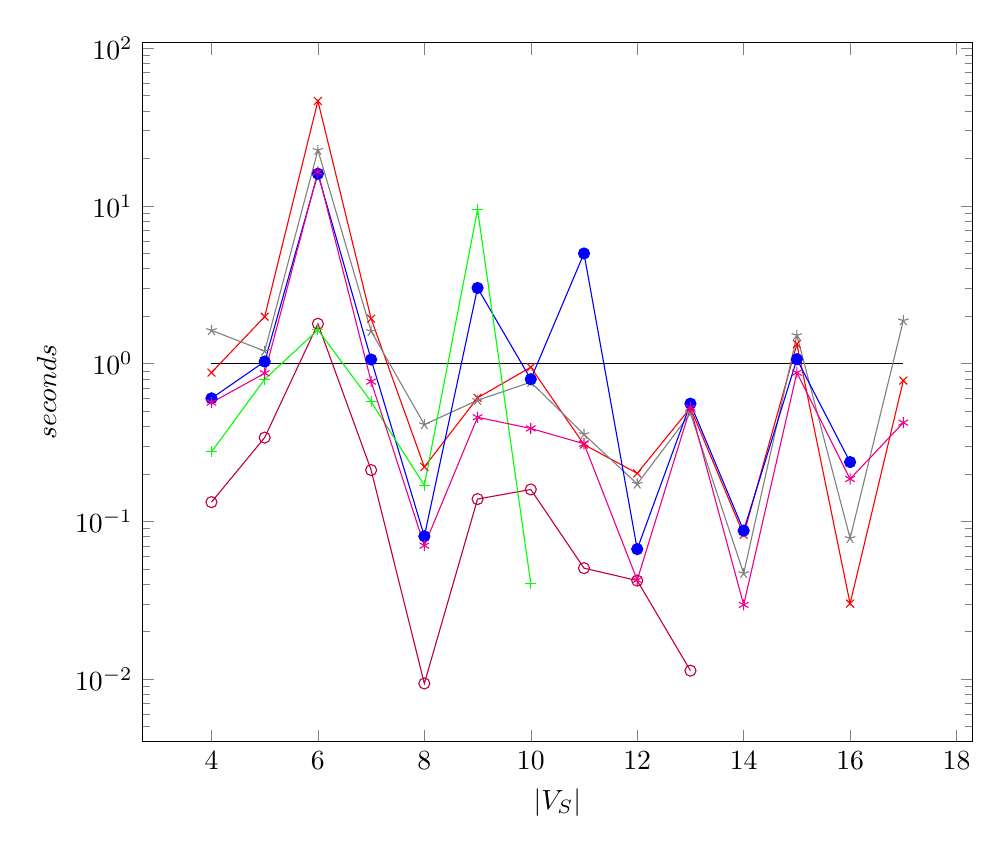
\begin{tikzpicture}
    \begin{axis}[
        xlabel=$|V_S|$,
        ylabel=$seconds$,
        ymode=log,
        legend style={at={(0.9,0.1)},anchor=south east},
        width=\textwidth,
		y tick label style={/pgf/number format/sci},
    ]


\addplot [mark=none, black] plot coordinates {
        (4,1) (17, 1)};
%\addlegendentry{No contraction}

	

  \addplot[
        mark=x,
        red,
    ] plot coordinates {
        (4,0.8783007924961822)
        (5,1.9866466250704127)
        (6,46.23915298831981)
        (7,1.9286013087935467)
        (8,0.22144887888388298)
        (9,0.6073880518853707)
        (10,0.9499470941285778)
        (11,0.3071513116204406)
        (12,0.20181763488775617)
        (13,0.5247142961355576)
        (14,0.08240035713162575)
        (15,1.3331646694970158)
        (16,0.030153907349204312)
        (17,0.7818188550294238)
};
%     \addlegendentry{DFS}

    \addplot[
        mark=o,
        purple,
    ] plot coordinates {
        (4,0.13253526170374963)
        (5,0.340135432164708)
        (6,1.790446045629151)
        (7,0.21172911942986739)
        (8,0.00939924729361108)
        (9,0.1386409264007632)
        (10,0.15954167221271842)
        (11,0.05059726207816495)
        (12,0.04218464066556149)
        (13,0.011328653011651979)
};
%    \addlegendentry{GDFS O IP}

 \addplot[
        mark=star,
        gray,
    ] plot coordinates {
        (4,1.6271054568492918)
        (5,1.2019347721569387)
        (6,22.57207288783596)
        (7,1.60714000055505)
        (8,0.41137411151774583)
        (9,0.5862167248296255)
        (10,0.7637400611154803)
        (11,0.356373039522627)
        (12,0.17288151392047257)
        (13,0.48433813085979627)
        (14,0.046838546665677216)
        (15,1.5140584943694408)
        (16,0.07823427303666675)
        (17,1.8750942580464485)
};
%    \addlegendentry{GDFS C}


\addplot[
        mark=*,
        blue,
    ] plot coordinates {
        (4,0.60298022841694)
        (5,1.0316944681766402)
        (6,15.991061194154563)
        (7,1.063190444555428)
        (8,0.08058508916228702)
        (9,3.019451686125926)
        (10,0.79704175618652)
        (11,4.998970774016183)
        (12,0.06678499576131569)
        (13,0.5580121902125518)
        (14,0.08746647794145956)
        (15,1.0672969432977613)
        (16,0.23788697499741307)
};
%    \addlegendentry{K-Path}

   \addplot[
        mark=+,
        green,
    ] plot coordinates {
        (4,0.2760410688096132)
        (5,0.7968662246398364)
        (6,1.6383115468640344)
        (7,0.5747225278886098)
        (8,0.16947067443329888)
        (9,9.48379348911334)
        (10,0.04037684393142793)
};
%    \addlegendentry{CP}
	\addplot[
        mark=asterisk,
        magenta,
    ] plot coordinates {
        (4,0.5669029018884123)
        (5,0.8690518164754274)
        (6,16.40156998152306)
        (7,0.7704428785494475)
        (8,0.07028167075789626)
        (9,0.4575408842013087)
        (10,0.38859339371640744)
        (11,0.31086090173433223)
        (12,0.0424840967267095)
        (13,0.5265194610065892)
        (14,0.02960328686421898)
        (15,0.8762590796270182)
        (16,0.1859213565027673)
        (17,0.42289838038406646)
};
%    \addlegendentry{GDFS A IP}

	
	
    \end{axis}
    \end{tikzpicture}

\caption{$|V_T|=5|V_S|$}
\label{fig:sub3}
\end{subfigure}
\begin{subfigure} {0.5\linewidth}
\centering

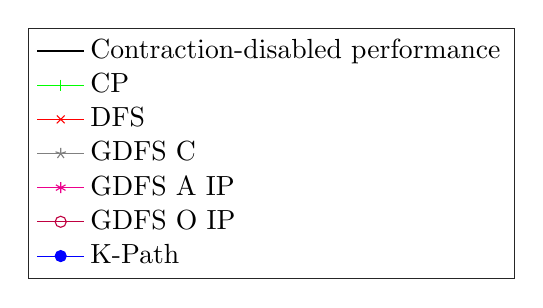
\begin{tikzpicture} 
    \begin{axis}[%
    hide axis,
    xmin=10,
    xmax=50,
    ymin=0,
    ymax=0.4,
    legend style={draw=white!15!black,legend cell align=left}
    ]
	\addlegendimage{black}
    \addlegendentry{Contraction-disabled performance}; 
     
    \addlegendimage{green, mark=+}
    \addlegendentry{CP};
    
    \addlegendimage{red, mark=x}
    \addlegendentry{DFS};
    
    \addlegendimage{gray, mark=star}
    \addlegendentry{GDFS C};
    
    \addlegendimage{magenta, mark=asterisk}
    \addlegendentry{GDFS A IP};
    
    \addlegendimage{purple, mark=o}
    \addlegendentry{GDFS O IP};
    
    \addlegendimage{blue, mark=*}
    \addlegendentry{K-Path};
    
    \end{axis}
\end{tikzpicture}

\end{subfigure}

\caption{Performance of using different path iterators in test cases with present subgraph homeomorphisms. We avoid unnecessary paths, We include a portfolio method that takes the best performance rating for each individual test case.}	
\label{fig:test}
\end{figure}





\begin{figure}
\begin{subfigure}{.5\linewidth}
\centering

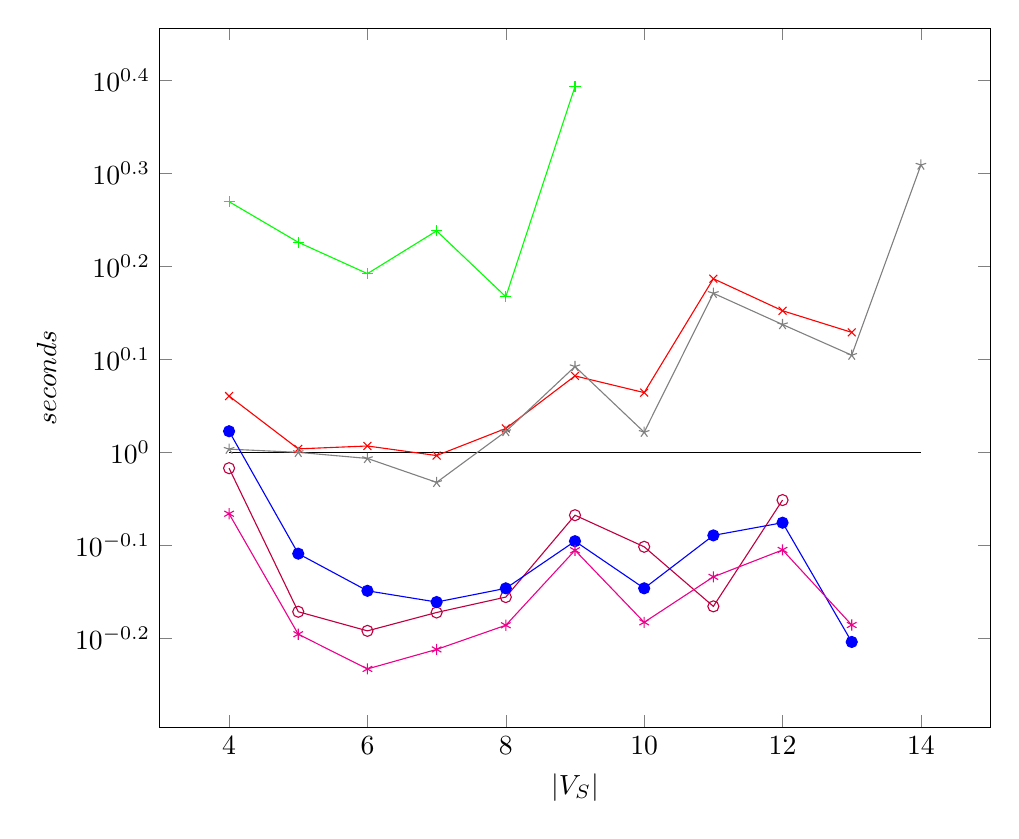
\begin{tikzpicture}
    \begin{axis}[
        xlabel=$|V_S|$,
        ylabel=$seconds$,
        ymode=log,
        legend style={at={(0.9,0.1)},anchor=south east},
        width=\textwidth,
		y tick label style={/pgf/number format/sci},
    ]
\addplot [mark=none, black] plot coordinates {
        (4,1) (14,1)};

   

\addplot[
        mark=x,
        red,
    ] plot coordinates {
        (4,1.149235278417448)
        (5,1.0083079007951214)
        (6,1.015552114217333)
        (7,0.9917637188145205)
        (8,1.060601873501574)
        (9,1.2080204277209134)
        (10,1.1590683500674202)
        (11,1.5368985401765969)
        (12,1.4196166165898805)
        (13,1.345479282144217)
};
%    \addlegendentry{DFS}


\addplot[
        mark=o,
        purple,
    ] plot coordinates {
        (4,0.9612291827097055)
        (5,0.6736846557006542)
        (6,0.6425091767491988)
        (7,0.6723934364944264)
        (8,0.6986220309175226)
        (9,0.8556489486454084)
        (10,0.7913299276289911)
        (11,0.6827413496042884)
        (12,0.8882442635255605)
};
%    \addlegendentry{GDFS O IP}


\addplot[
        mark=star,
        gray,
    ] plot coordinates {
        (4,1.0076438451392467)
        (5,0.9996588783961261)
        (6,0.9847179505164285)
        (7,0.9280395733234135)
        (8,1.052698920988995)
        (9,1.2364165435036165)
        (10,1.0508458659524293)
        (11,1.482398673483428)
        (12,1.3719047068368444)
        (13,1.2716510858517898)
        (14,2.0364819148591398)
};
%    \addlegendentry{GDFS C}


\addplot[
        mark=*,
        blue,
    ] plot coordinates {
        (4,1.0533520014717994)
        (5,0.7778922096030297)
        (6,0.7095420859821555)
        (7,0.690031519800899)
        (8,0.7138989512612041)
        (9,0.8022495198052423)
        (10,0.7139100327511367)
        (11,0.8138526765920138)
        (12,0.839844649957909)
        (13,0.6251267562387761)
};
%    \addlegendentry{K-Path}


\addplot[
        mark=+,
        green,
    ] plot coordinates {
        (4,1.8598817420849323)
        (5,1.6819321086529642)
        (6,1.5562633425290353)
        (7,1.7300402065586273)
        (8,1.4697328084299048)
        (9,2.4737693466393464)
};
%    \addlegendentry{CP}


\addplot[
        mark=asterisk,
        magenta,
    ] plot coordinates {
        (4,0.8587470004926293)
        (5,0.637211123426433)
        (6,0.5846797577876022)
        (7,0.6136474407419334)
        (8,0.6515146194296546)
        (9,0.7843995636829644)
        (10,0.6563231931888491)
        (11,0.7344868290598967)
        (12,0.7852380262879831)
        (13,0.6519427807384649)
};
%    \addlegendentry{GDFS A IP}


   

    \end{axis}
    \end{tikzpicture}


\caption{Serial}
\label{fig:sub1}
\end{subfigure}%
\begin{subfigure}{.5\linewidth}
\centering

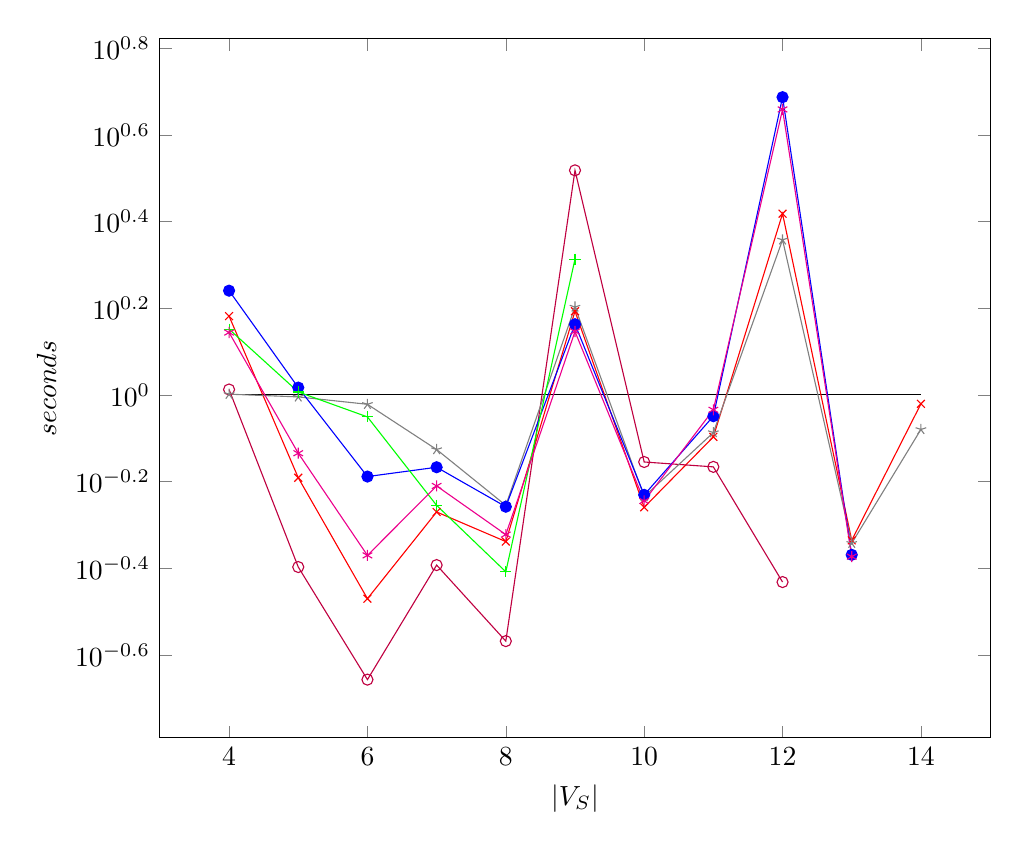
\begin{tikzpicture}
    \begin{axis}[
        xlabel=$|V_S|$,
        ylabel=$seconds$,
        ymode=log,
        legend style={at={(0.9,0.1)},anchor=south east},
        width=\textwidth,
		y tick label style={/pgf/number format/sci},
    ]
\addplot [mark=none, black] plot coordinates {
        (4,1) (14, 1)};




\addplot[
        mark=x,
        red,
    ] plot coordinates {
        (4,1.5196735481803552)
        (5,0.6439969153711)
        (6,0.3386925334619767)
        (7,0.5368610674342231)
        (8,0.45873474922274815)
        (9,1.5594868514866573)
        (10,0.5503271443080898)
        (11,0.8002158520089797)
        (12,2.618829716025611)
        (13,0.461660681606467)
        (14,0.9536983450489754)
};
%    \addlegendentry{DFS}


\addplot[
        mark=o,
        purple,
    ] plot coordinates {
        (4,1.0289639751297441)
        (5,0.40073099730691264)
        (6,0.2203309298278896)
        (7,0.40490458510733796)
        (8,0.2703553467095787)
        (9,3.2968841136523857)
        (10,0.7001969451830652)
        (11,0.6822506009880664)
        (12,0.37004898049509893)
};
%    \addlegendentry{GDFS O IP}


\addplot[
        mark=star,
        gray,
    ] plot coordinates {
        (4,1.0037860591934256)
        (5,0.9894012765779054)
        (6,0.9512995639254895)
        (7,0.7481500768569231)
        (8,0.5560328419142169)
        (9,1.5950594125932698)
        (10,0.5825880979420317)
        (11,0.8186254429321587)
        (12,2.2787645869722217)
        (13,0.4547207271773557)
        (14,0.8323681075075677)
};
%    \addlegendentry{GDFS C}


\addplot[
        mark=*,
        blue,
    ] plot coordinates {
        (4,1.739824792303458)
        (5,1.0396016144545588)
        (6,0.6479907091747379)
        (7,0.6809036260493723)
        (8,0.5520901104899674)
        (9,1.4556125513833869)
        (10,0.5879764504015326)
        (11,0.8930337054115022)
        (12,4.862531350090637)
        (13,0.4275493552859416)
};
%    \addlegendentry{K-Path}


\addplot[
        mark=+,
        green,
    ] plot coordinates {
        (4,1.4181640975707355)
        (5,1.0155919393670438)
        (6,0.8896407770170547)
        (7,0.5560547295333215)
        (8,0.3908257237814686)
        (9,2.0567874784311706)
};
%    \addlegendentry{CP}


\addplot[
        mark=asterisk,
        magenta,
    ] plot coordinates {
        (4,1.3928057135978327)
        (5,0.7336372164409364)
        (6,0.4262986752445699)
        (7,0.6165329994701355)
        (8,0.47610065673013646)
        (9,1.4003560173584488)
        (10,0.5691849125616277)
        (11,0.9238715681263124)
        (12,4.55583983031228)
        (13,0.4234248244588815)
};
%    \addlegendentry{GDFS A IP}
  

	
    \end{axis}
    \end{tikzpicture}

\caption{Cached}
\label{fig:sub2}
\end{subfigure}\\[1ex]
\begin{subfigure}{0.5\linewidth}
\centering

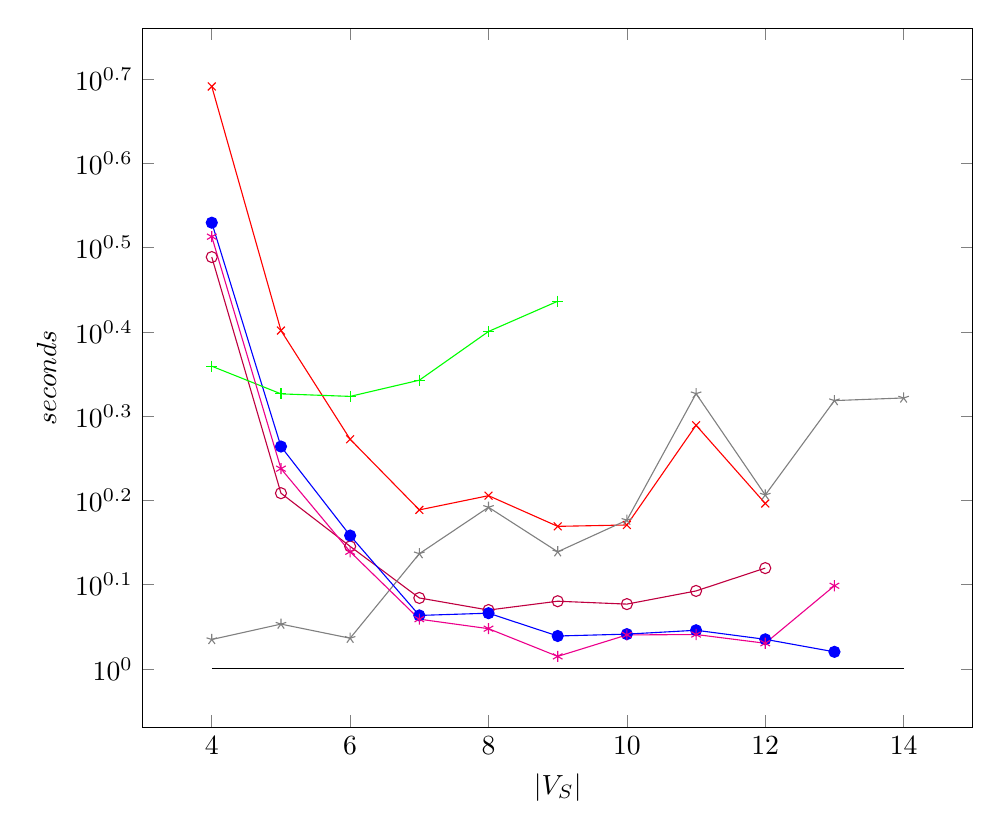
\begin{tikzpicture}
    \begin{axis}[
        xlabel=$|V_S|$,
        ylabel=$seconds$,
        ymode=log,
        legend style={at={(0.9,0.1)},anchor=south east},
        width=\textwidth,
		y tick label style={/pgf/number format/sci},
    ]
\addplot [mark=none, black] plot coordinates {
        (4,1) (14, 1)};


	

\addplot[
        mark=x,
        red,
    ] plot coordinates {
        (4,4.912635821328207)
        (5,2.5213322807291894)
        (6,1.8735281366916912)
        (7,1.5444862545247475)
        (8,1.6056787150146559)
        (9,1.4765521555469698)
        (10,1.4820555556240134)
        (11,1.946734238439349)
        (12,1.5718556269712267)
};
%    \addlegendentry{DFS}


\addplot[
        mark=o,
        purple,
    ] plot coordinates {
        (4,3.0822240524751128)
        (5,1.6165571205344698)
        (6,1.3978485397981901)
        (7,1.2140415216311997)
        (8,1.1745946191206549)
        (9,1.2032865829671746)
        (10,1.1937969470403793)
        (11,1.2375642924085462)
        (12,1.3172897955473268)
};
%    \addlegendentry{GDFS O IP}


\addplot[
        mark=star,
        gray,
    ] plot coordinates {
        (4,1.0837979979749324)
        (5,1.1303336976253304)
        (6,1.087572597425233)
        (7,1.3702576979065668)
        (8,1.5556435786427398)
        (9,1.3774635843717524)
        (10,1.5016451292498205)
        (11,2.122041244880633)
        (12,1.6087569895860554)
        (13,2.0820432556276365)
        (14,2.09712979447583)
};
%    \addlegendentry{GDFS C}


\addplot[
        mark=*,
        blue,
    ] plot coordinates {
        (4,3.38561160720786)
        (5,1.8365969772716313)
        (6,1.4398010790115316)
        (7,1.1574587494667208)
        (8,1.1645623226507533)
        (9,1.0941954726393444)
        (10,1.099782306968)
        (11,1.1114580211799494)
        (12,1.0842992282419759)
        (13,1.0478118522343631)
};
%    \addlegendentry{K-Path}


\addplot[
        mark=+,
        green,
    ] plot coordinates {
        (4,2.287168110582633)
        (5,2.120634315355006)
        (6,2.1061165486427873)
        (7,2.2013837152903006)
        (8,2.514842573582901)
        (9,2.731646143463003)
};
%    \addlegendentry{CP}


\addplot[
        mark=asterisk,
        magenta,
    ] plot coordinates {
        (4,3.2585173952994615)
        (5,1.728583400469593)
        (6,1.3775627829587174)
        (7,1.1456803324069784)
        (8,1.1162737735571762)
        (9,1.0349155153974534)
        (10,1.0973729419863378)
        (11,1.098601313310929)
        (12,1.0726988929900587)
        (13,1.2552103868339886)
};
%    \addlegendentry{GDFS A IP}

	
	
    \end{axis}
    \end{tikzpicture}

\caption{Parallel}
\label{fig:sub3}
\end{subfigure}
\begin{subfigure} {0.5\linewidth}
\centering

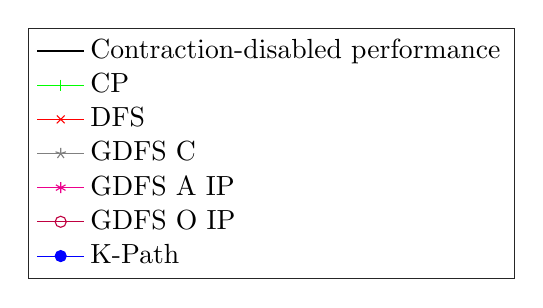
\begin{tikzpicture} 
    \begin{axis}[%
    hide axis,
    xmin=10,
    xmax=50,
    ymin=0,
    ymax=0.4,
    legend style={draw=white!15!black,legend cell align=left}
    ]
	\addlegendimage{black}
    \addlegendentry{Contraction-disabled performance}; 
     
    \addlegendimage{green, mark=+}
    \addlegendentry{CP};
    
    \addlegendimage{red, mark=x}
    \addlegendentry{DFS};
    
    \addlegendimage{gray, mark=star}
    \addlegendentry{GDFS C};
    
    \addlegendimage{magenta, mark=asterisk}
    \addlegendentry{GDFS A IP};
    
    \addlegendimage{purple, mark=o}
    \addlegendentry{GDFS O IP};
    
    \addlegendimage{blue, mark=*}
    \addlegendentry{K-Path};
    
    \end{axis}
\end{tikzpicture}

\end{subfigure}

\caption{Performance of our algorithm with \textbf{ZeroDomain} pruning using \textbf{`Labels and neighbours'} filtering relative to the performance of the algorithm without pruning. We avoid unnecessarily long paths, do not perform contraction and use the degree-based target graph vertex ordering. Data points above the black reference line denote that the pruning method introduces more delay, and data points below the reference line denote that the pruning method saves time. Note the logarithmic y-axis.}	
\label{fig:test}
\end{figure}


\begin{figure}
\begin{subfigure}{.5\linewidth}
\centering

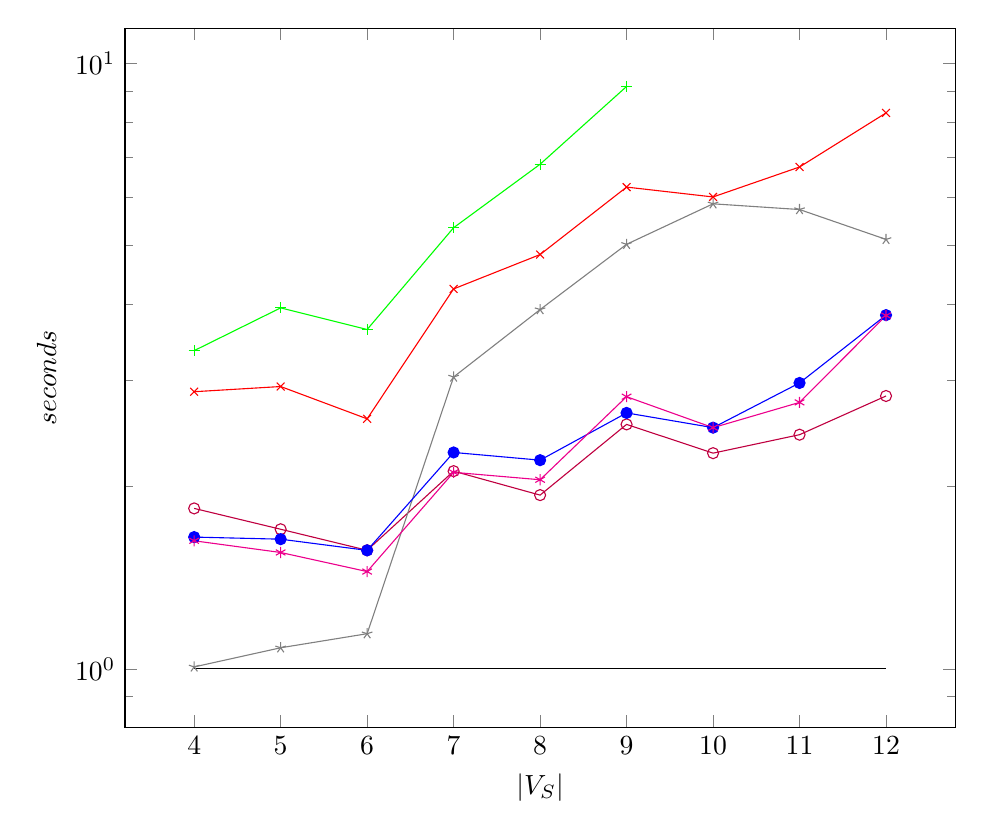
\begin{tikzpicture}
    \begin{axis}[
        xlabel=$|V_S|$,
        ylabel=$seconds$,
        ymode=log,
        legend style={at={(0.9,0.1)},anchor=south east},
        width=\textwidth,
		y tick label style={/pgf/number format/sci},
    ]
\addplot [mark=none, black] plot coordinates {
        (4,1) (12, 1)};

    

\addplot[
        mark=x,
        red,
    ] plot coordinates {
        (4,2.8681701535417203)
        (5,2.9254018783511473)
        (6,2.5872798141640203)
        (7,4.239345235159544)
        (8,4.830571894920121)
        (9,6.242761798378523)
        (10,6.013058042923716)
        (11,6.738597774875578)
        (12,8.275599621231075)
};
%    \addlegendentry{DFS}


\addplot[
        mark=o,
        purple,
    ] plot coordinates {
        (4,1.8408080356188123)
        (5,1.7005582324670065)
        (6,1.56989493549955)
        (7,2.1207796500463942)
        (8,1.9363735218126932)
        (9,2.533248243975908)
        (10,2.2707880019469786)
        (11,2.4359352917004715)
        (12,2.821912275157622)
};
%    \addlegendentry{GDFS O IP}


\addplot[
        mark=star,
        gray,
    ] plot coordinates {
        (4,1.0076654131165232)
        (5,1.0837612058063686)
        (6,1.1432927339149115)
        (7,3.033634347762899)
        (8,3.919309944661518)
        (9,5.022580039736159)
        (10,5.858260568094502)
        (11,5.732626441781628)
        (12,5.117036438110539)
};
%    \addlegendentry{GDFS C}


\addplot[
        mark=*,
        blue,
    ] plot coordinates {
        (4,1.6507129093587034)
        (5,1.6376785905633322)
        (6,1.5694034681484315)
        (7,2.2768378662823556)
        (8,2.2111751094243637)
        (9,2.6460554936280003)
        (10,2.5019612966868143)
        (11,2.9653929534687484)
        (12,3.8377325981845987)
};
%    \addlegendentry{K-Path}


\addplot[
        mark=+,
        green,
    ] plot coordinates {
        (4,3.3530620508044278)
        (5,3.945082943073584)
        (6,3.633181121338477)
        (7,5.349792316707754)
        (8,6.809444287637352)
        (9,9.151106021332374)
};
%    \addlegendentry{CP}


\addplot[
        mark=asterisk,
        magenta,
    ] plot coordinates {
        (4,1.6276085621719778)
        (5,1.5567783428027056)
        (6,1.447868814386046)
        (7,2.111238924804706)
        (8,2.052589583126582)
        (9,2.8147150464658517)
        (10,2.5017899929941634)
        (11,2.7540625611814193)
        (12,3.831399427105856)
};
%    \addlegendentry{GDFS A IP}

   

    \end{axis}
    \end{tikzpicture}


\caption{serial}
\label{fig:sub1}
\end{subfigure}%
\begin{subfigure}{.5\linewidth}
\centering

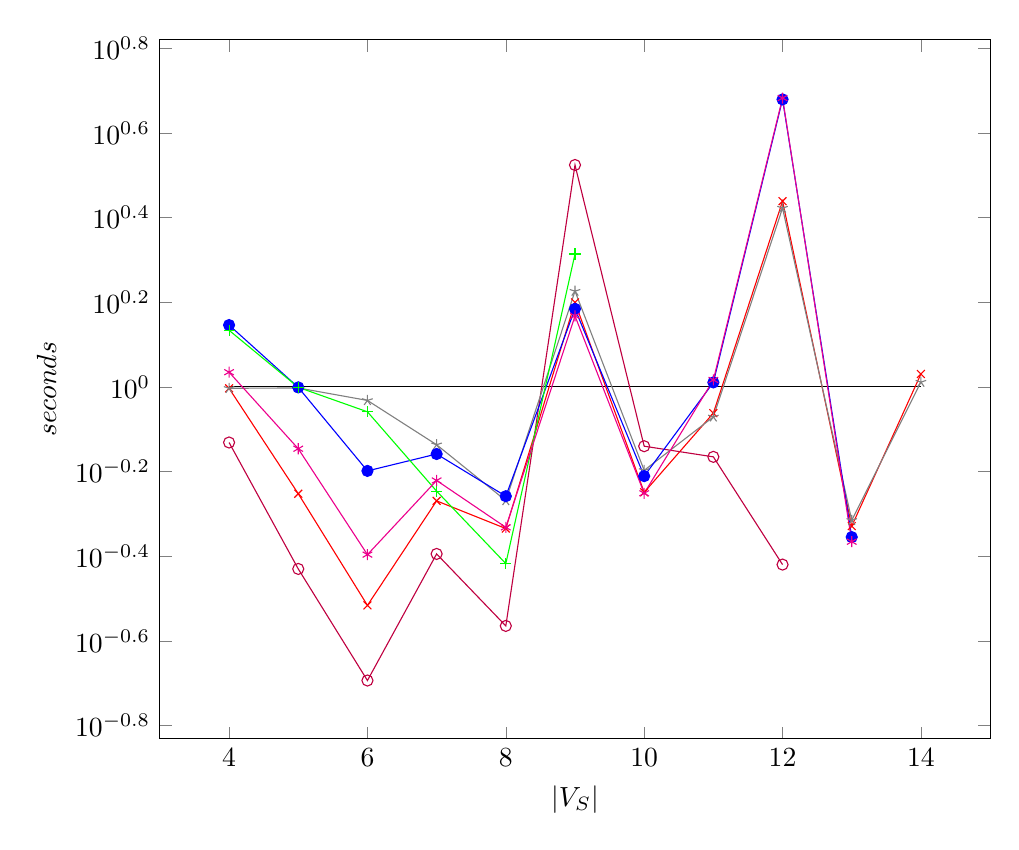
\begin{tikzpicture}
    \begin{axis}[
        xlabel=$|V_S|$,
        ylabel=$seconds$,
        ymode=log,
        legend style={at={(0.9,0.1)},anchor=south east},
        width=\textwidth,
		y tick label style={/pgf/number format/sci},
    ]
\addplot [mark=none, black] plot coordinates {
        (4,1) (14, 1)};


	

\addplot[
        mark=x,
        red,
    ] plot coordinates {
        (4,0.9923899104921649)
        (5,0.5595066683253078)
        (6,0.3048945865180337)
        (7,0.5381004704636452)
        (8,0.4628899334014771)
        (9,1.5833880688615796)
        (10,0.563696852962109)
        (11,0.8669963898068426)
        (12,2.745349524198522)
        (13,0.4690924414042419)
        (14,1.0728242665153411)
};
%    \addlegendentry{DFS}


\addplot[
        mark=o,
        purple,
    ] plot coordinates {
        (4,0.739244200124882)
        (5,0.3717240182715724)
        (6,0.20260979424571846)
        (7,0.40328082248328134)
        (8,0.2726428806815875)
        (9,3.342614987755728)
        (10,0.7244476709108397)
        (11,0.6836929828863543)
        (12,0.3805696273086222)
};
%    \addlegendentry{GDFS O IP}


\addplot[
        mark=star,
        gray,
    ] plot coordinates {
        (4,0.9924896603950555)
        (5,0.994360434712658)
        (6,0.9291538705872268)
        (7,0.730196682594658)
        (8,0.5390873818404287)
        (9,1.6832008614785352)
        (10,0.6352356062289578)
        (11,0.8496501176486361)
        (12,2.6445551844487807)
        (13,0.4840033554409139)
        (14,1.026259804661441)
};
%    \addlegendentry{GDFS C}


\addplot[
        mark=*,
        blue,
    ] plot coordinates {
        (4,1.3997982449312394)
        (5,0.997525391259792)
        (6,0.6333756640426693)
        (7,0.6943303320196079)
        (8,0.5519684346380963)
        (9,1.5286729452268917)
        (10,0.6156583962202479)
        (11,1.024740262929912)
        (12,4.774734990588401)
        (13,0.4419374709287728)
};
%    \addlegendentry{K-Path}


\addplot[
        mark=+,
        green,
    ] plot coordinates {
        (4,1.3603876642406472)
        (5,0.9977315311707801)
        (6,0.8734385188908586)
        (7,0.5673919611448295)
        (8,0.3826349700684204)
        (9,2.0597652911938544)
};
%    \addlegendentry{CP}


\addplot[
        mark=asterisk,
        magenta,
    ] plot coordinates {
        (4,1.0832036968767507)
        (5,0.714551103294575)
        (6,0.4017364306204272)
        (7,0.6012055707935953)
        (8,0.4660022392983759)
        (9,1.4709429657453295)
        (10,0.5607915060867077)
        (11,1.0386348465457822)
        (12,4.8097603627365055)
        (13,0.43097398458603053)
};
%    \addlegendentry{GDFS A IP}

	
    \end{axis}
    \end{tikzpicture}

\caption{cached}
\label{fig:sub2}
\end{subfigure}\\[1ex]
\begin{subfigure}{0.5\linewidth}
\centering

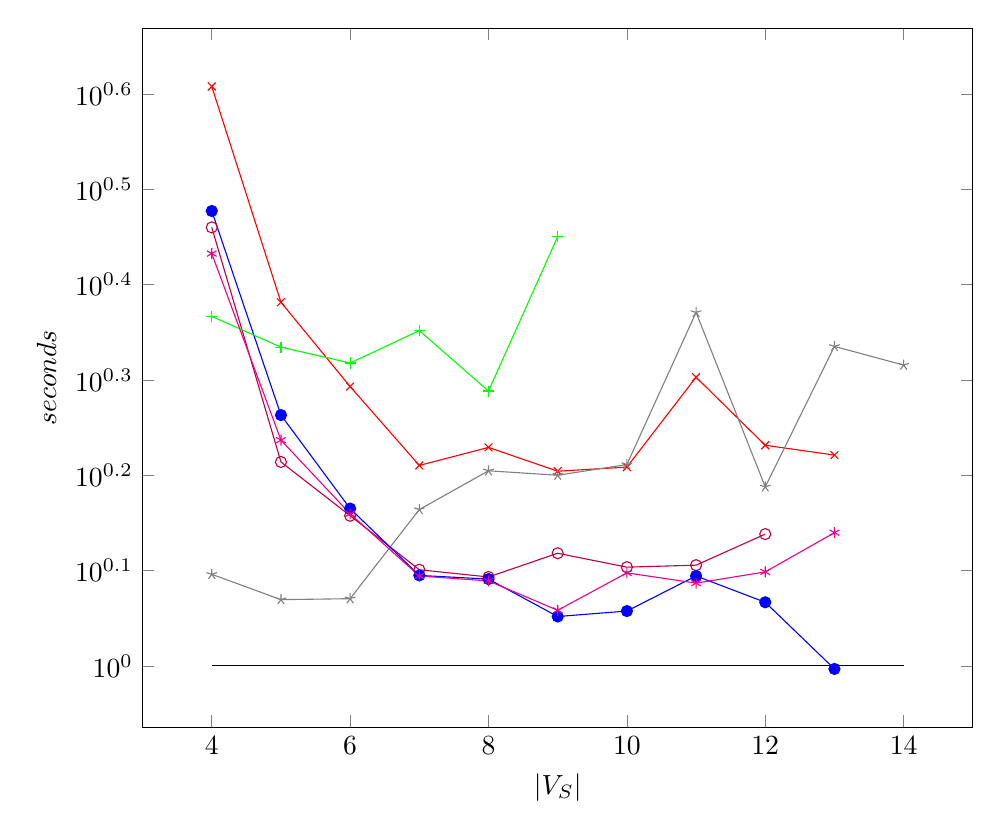
\begin{tikzpicture}
    \begin{axis}[
        xlabel=$|V_S|$,
        ylabel=$seconds$,
        ymode=log,
        legend style={at={(0.9,0.1)},anchor=south east},
        width=\textwidth,
		y tick label style={/pgf/number format/sci},
    ]
\addplot [mark=none, black] plot coordinates {
        (4,1) (14, 1)};



\addplot[
        mark=x,
        red,
    ] plot coordinates {
        (4,4.055665332528571)
        (5,2.4079068291217)
        (6,1.9643320384841314)
        (7,1.6232718485965263)
        (8,1.6955903014633646)
        (9,1.6008062270872792)
        (10,1.6167961960677952)
        (11,2.008933357310069)
        (12,1.704410962543426)
        (13,1.6643657926641058)
};
%    \addlegendentry{DFS}


\addplot[
        mark=o,
        purple,
    ] plot coordinates {
        (4,2.8851878090262195)
        (5,1.636942509871993)
        (6,1.4374997042728976)
        (7,1.2616655204621405)
        (8,1.2396952026488233)
        (9,1.3129460412244731)
        (10,1.269489134852407)
        (11,1.2756554118663406)
        (12,1.3750472085101815)
};
%    \addlegendentry{GDFS O IP}


\addplot[
        mark=star,
        gray,
    ] plot coordinates {
        (4,1.2478328793750295)
        (5,1.1736817816635776)
        (6,1.1764101574372858)
        (7,1.4592075490444798)
        (8,1.6024676243054734)
        (9,1.5853180312626138)
        (10,1.6267475153944102)
        (11,2.3492273224066422)
        (12,1.541367629203128)
        (13,2.1643253277100984)
        (14,2.068648556937112)
};
%    \addlegendentry{GDFS C}


\addplot[
        mark=*,
        blue,
    ] plot coordinates {
        (4,3.002052014953125)
        (5,1.8333632864658882)
        (6,1.4625868876088735)
        (7,1.244428892395309)
        (8,1.2334917943953325)
        (9,1.1267969028185083)
        (10,1.1417960691621196)
        (11,1.242845045792521)
        (12,1.1662050312002787)
        (13,0.9927656897482176)
};
%    \addlegendentry{K-Path}


\addplot[
        mark=+,
        green,
    ] plot coordinates {
        (4,2.327075300876756)
        (5,2.160407689989366)
        (6,2.0792574180238432)
        (7,2.248434541176637)
        (8,1.943200046149185)
        (9,2.82171519727411)
};
%    \addlegendentry{CP}


\addplot[
        mark=asterisk,
        magenta,
    ] plot coordinates {
        (4,2.7083657638964724)
        (5,1.7258042096013082)
        (6,1.4441565938470444)
        (7,1.2427090481371263)
        (8,1.2279821585739619)
        (9,1.1438554945469597)
        (10,1.252073988123748)
        (11,1.2215012813271526)
        (12,1.2550832966834882)
        (13,1.3798442157135253)
};
%    \addlegendentry{GDFS A IP}

	
    \end{axis}
    \end{tikzpicture}

\caption{parallel}
\label{fig:sub3}
\end{subfigure}
\begin{subfigure} {0.5\linewidth}
\centering

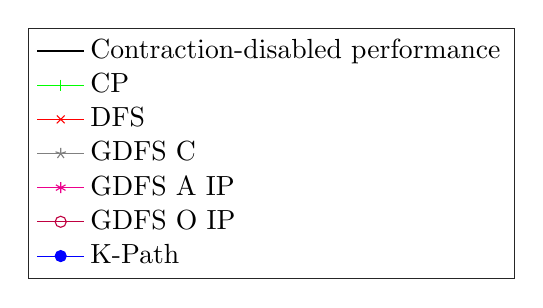
\begin{tikzpicture} 
    \begin{axis}[%
    hide axis,
    xmin=10,
    xmax=50,
    ymin=0,
    ymax=0.4,
    legend style={draw=white!15!black,legend cell align=left}
    ]
	\addlegendimage{black}
    \addlegendentry{Contraction-disabled performance}; 
     
    \addlegendimage{green, mark=+}
    \addlegendentry{CP};
    
    \addlegendimage{red, mark=x}
    \addlegendentry{DFS};
    
    \addlegendimage{gray, mark=star}
    \addlegendentry{GDFS C};
    
    \addlegendimage{magenta, mark=asterisk}
    \addlegendentry{GDFS A IP};
    
    \addlegendimage{purple, mark=o}
    \addlegendentry{GDFS O IP};
    
    \addlegendimage{blue, mark=*}
    \addlegendentry{K-Path};
    
    \end{axis}
\end{tikzpicture}

\end{subfigure}

\caption{Performance of our algorithm with \textbf{ZeroDomain} pruning using \textbf{`Free neighbours'} filtering relative to the performance of the algorithm without pruning. We avoid unnecessarily long paths, do not perform contraction and use the degree-based target graph vertex ordering. Data points above the black reference line denote that the pruning method introduces more delay, and data points below the reference line denote that the pruning method saves time. Note the logarithmic y-axis.}	
\label{fig:test}
\end{figure}

\begin{figure}
\begin{subfigure}{.5\linewidth}
\centering

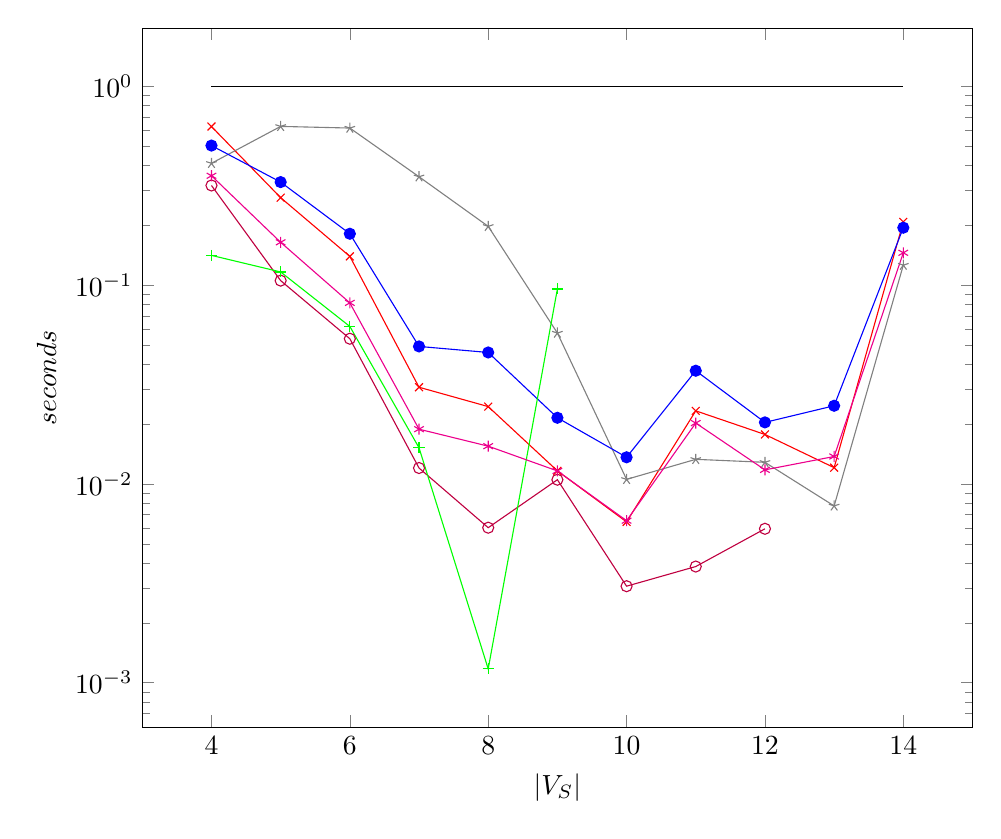
\begin{tikzpicture}
        \begin{axis}[
        xlabel=$|V_S|$,
        ylabel=$seconds$,
        ymode=log,
        legend style={at={(0.9,0.1)},anchor=south east},
        width=\textwidth,
		y tick label style={/pgf/number format/sci},
    ]
\addplot [mark=none, black] plot coordinates {
        (4,1) (14, 1)};



\addplot[
        mark=x,
        red,
    ] plot coordinates {
        (4,0.6287543277612293)
        (5,0.2757977099154991)
        (6,0.1396777930920231)
        (7,0.030673609879429353)
        (8,0.02451224889378789)
        (9,0.011639988009323088)
        (10,0.006444926208946211)
        (11,0.023332165971646113)
        (12,0.017747881691377088)
        (13,0.012081584812504542)
        (14,0.20827170338997036)
};
%    \addlegendentry{DFS}


\addplot[
        mark=o,
        purple,
    ] plot coordinates {
        (4,0.31762184661225146)
        (5,0.10548661997054809)
        (6,0.05380597268481946)
        (7,0.012031104647835078)
        (8,0.006026685633755746)
        (9,0.010506576117209399)
        (10,0.003059622842895182)
        (11,0.0038425576274282447)
        (12,0.005950005569221872)
};
%    \addlegendentry{GDFS O IP}


\addplot[
        mark=star,
        gray,
    ] plot coordinates {
        (4,0.4106300255336265)
        (5,0.6297150335729914)
        (6,0.6177849466375939)
        (7,0.3514224232413242)
        (8,0.1978056188420405)
        (9,0.05747899493182684)
        (10,0.01054844071183747)
        (11,0.013304423784248232)
        (12,0.01285276131493418)
        (13,0.007754862312966293)
        (14,0.12620402164239297)
};
%    \addlegendentry{GDFS C}


\addplot[
        mark=*,
        blue,
    ] plot coordinates {
        (4,0.5042771733798161)
        (5,0.33026481004490515)
        (6,0.1815749814615767)
        (7,0.04920860049799136)
        (8,0.04588175630434421)
        (9,0.02153377003082302)
        (10,0.013622516633218007)
        (11,0.037145391651794424)
        (12,0.02041196505471854)
        (13,0.024748365975288622)
        (14,0.19477391590054371)
};
%    \addlegendentry{K-Path}


\addplot[
        mark=+,
        green,
    ] plot coordinates {
        (4,0.14129388384266495)
        (5,0.11661297643581336)
        (6,0.062037664925466474)
        (7,0.015214384516616386)
        (8,0.001173447995948207)
        (9,0.09577023175742294)
};
%    \addlegendentry{CP}


\addplot[
        mark=asterisk,
        magenta,
    ] plot coordinates {
        (4,0.35547913440959544)
        (5,0.16441492185647066)
        (6,0.081522356518962)
        (7,0.01887115321256927)
        (8,0.015496754850373495)
        (9,0.01163137758041799)
        (10,0.0065360121014294)
        (11,0.02025243713993974)
        (12,0.011777226097555493)
        (13,0.013750262714309236)
        (14,0.1456191628467376)
};
%    \addlegendentry{GDFS A IP}


   

    \end{axis}
    \end{tikzpicture}


\caption{serial}
\label{fig:sub1}
\end{subfigure}%
\begin{subfigure}{.5\linewidth}
\centering

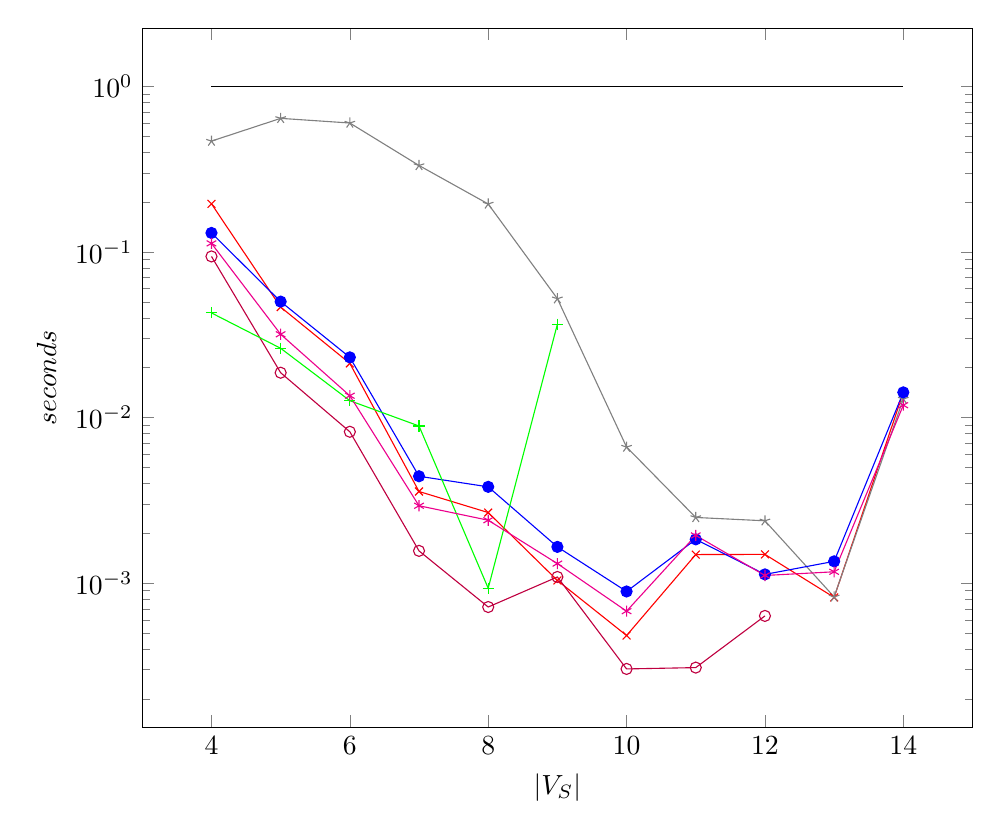
\begin{tikzpicture}
       \begin{axis}[
        xlabel=$|V_S|$,
        ylabel=$seconds$,
        ymode=log,
        legend style={at={(0.9,0.1)},anchor=south east},
        width=\textwidth,
		y tick label style={/pgf/number format/sci},
    ]
\addplot [mark=none, black] plot coordinates {
        (4,1) (14, 1)};



\addplot[
        mark=x,
        red,
    ] plot coordinates {
        (4,0.19553736011435197)
        (5,0.04651353813878456)
        (6,0.021254007864093483)
        (7,0.003578003137043706)
        (8,0.002669239461236206)
        (9,0.001038638013086457)
        (10,4.827831034437402E-4)
        (11,0.0014882311568104045)
        (12,0.0014918153191871841)
        (13,8.201888846909311E-4)
        (14,0.014177555092282024)
};
%    \addlegendentry{DFS}


\addplot[
        mark=o,
        purple,
    ] plot coordinates {
        (4,0.0940851187730316)
        (5,0.018669179394963042)
        (6,0.008210777047784168)
        (7,0.00156671351986859)
        (8,7.175769161658074E-4)
        (9,0.0010901108792181757)
        (10,3.032823855272371E-4)
        (11,3.089718288207255E-4)
        (12,6.339461008270098E-4)
};
%    \addlegendentry{GDFS O IP}


\addplot[
        mark=star,
        gray,
    ] plot coordinates {
        (4,0.46776174984809504)
        (5,0.6418994975058616)
        (6,0.6016705469416976)
        (7,0.33331288068306)
        (8,0.19516359829459384)
        (9,0.052258028899510256)
        (10,0.00663966390973203)
        (11,0.002493325643069144)
        (12,0.002380331383759815)
        (13,8.261279519951037E-4)
        (14,0.012952744336981126)
};
%    \addlegendentry{GDFS C}


\addplot[
        mark=*,
        blue,
    ] plot coordinates {
        (4,0.13042500432875637)
        (5,0.050180114187121205)
        (6,0.023114568588865403)
        (7,0.004422648284462927)
        (8,0.0038176084846363034)
        (9,0.0016559892479824923)
        (10,8.905816418131041E-4)
        (11,0.0018391391340257801)
        (12,0.0011295780527541543)
        (13,0.0013542664491973389)
        (14,0.01420206790590417)
};
%    \addlegendentry{K-Path}


\addplot[
        mark=+,
        green,
    ] plot coordinates {
        (4,0.0428754303586345)
        (5,0.026223845245723965)
        (6,0.012652891562625723)
        (7,0.008896499518256218)
        (8,9.31591774671725E-4)
        (9,0.03666836072401081)
};
%    \addlegendentry{CP}


\addplot[
        mark=asterisk,
        magenta,
    ] plot coordinates {
        (4,0.11278665322864612)
        (5,0.03186942103424617)
        (6,0.013551849864991583)
        (7,0.0029347571062988687)
        (8,0.0023993757390741166)
        (9,0.001312317141160979)
        (10,6.774056453796584E-4)
        (11,0.0019421604989434682)
        (12,0.0011128003583009694)
        (13,0.0011711624655019737)
        (14,0.011878755635911897)
};
%    \addlegendentry{GDFS A IP}

	
	
    \end{axis}
    \end{tikzpicture}

\caption{cached}
\label{fig:sub2}
\end{subfigure}\\[1ex]
\begin{subfigure}{0.5\linewidth}
\centering

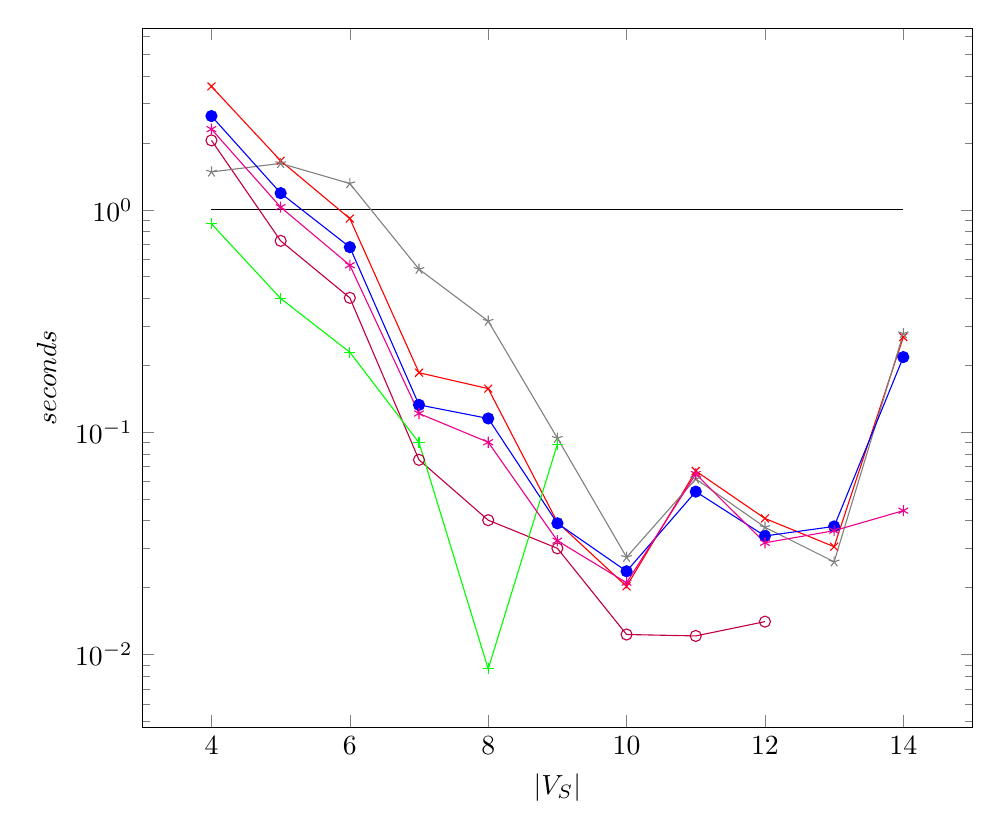
\begin{tikzpicture}
    \begin{axis}[
        xlabel=$|V_S|$,
        ylabel=$seconds$,
        ymode=log,
        legend style={at={(0.9,0.1)},anchor=south east},
        width=\textwidth,
		y tick label style={/pgf/number format/sci},
    ]
\addplot [mark=none, black] plot coordinates {
        (4,1) (14, 1)};



\addplot[
        mark=x,
        red,
    ] plot coordinates {
        (4,3.5863917566717767)
        (5,1.6614170135257829)
        (6,0.913341561725058)
        (7,0.18513401953197028)
        (8,0.15706371851369083)
        (9,0.039380360092514)
        (10,0.020272354245869484)
        (11,0.06693875268275729)
        (12,0.04094655208604481)
        (13,0.03057385975605409)
        (14,0.26792292492149405)
};
%    \addlegendentry{DFS}


\addplot[
        mark=o,
        purple,
    ] plot coordinates {
        (4,2.052763630992859)
        (5,0.7252220094219901)
        (6,0.4019908919869054)
        (7,0.0751392967924247)
        (8,0.0402321588998491)
        (9,0.030063816263190213)
        (10,0.012316567212513396)
        (11,0.012136049821184658)
        (12,0.01407028044173897)
};
%    \addlegendentry{GDFS O IP}


\addplot[
        mark=star,
        gray,
    ] plot coordinates {
        (4,1.4803263312981985)
        (5,1.617088480231661)
        (6,1.312985590310922)
        (7,0.541000232064156)
        (8,0.31621413493384876)
        (9,0.09404453831749748)
        (10,0.027408496020476347)
        (11,0.061673144974397576)
        (12,0.03739780619521971)
        (13,0.02614141264184211)
        (14,0.2777072903785752)
};
%    \addlegendentry{GDFS C}


\addplot[
        mark=*,
        blue,
    ] plot coordinates {
        (4,2.640444380229205)
        (5,1.1886881061231498)
        (6,0.6793824205820389)
        (7,0.13271318550783862)
        (8,0.11533183769943123)
        (9,0.038955674057646106)
        (10,0.023698433402264296)
        (11,0.0540615523126724)
        (12,0.034171466937311545)
        (13,0.03771279726019261)
        (14,0.21769075053049192)
};
%    \addlegendentry{K-Path}


\addplot[
        mark=+,
        green,
    ] plot coordinates {
        (4,0.8650360306803884)
        (5,0.39951182944872243)
        (6,0.2288811300337159)
        (7,0.0896782754536235)
        (8,0.008624199068128502)
        (9,0.08847130248188806)
};
%    \addlegendentry{CP}


\addplot[
        mark=asterisk,
        magenta,
    ] plot coordinates {
        (4,2.3056130434020963)
        (5,1.0279513694895468)
        (6,0.5632528558219363)
        (7,0.12138481892093078)
        (8,0.09017283243188468)
        (9,0.03252156535486139)
        (10,0.02104885765787201)
        (11,0.06488806314689854)
        (12,0.031829464045399214)
        (13,0.03607848508196143)
        (14,0.04438987254212279)
};
%    \addlegendentry{GDFS A IP}

	
    \end{axis}
    \end{tikzpicture}

\caption{parallel}
\label{fig:sub3}
\end{subfigure}
\begin{subfigure} {0.5\linewidth}
\centering

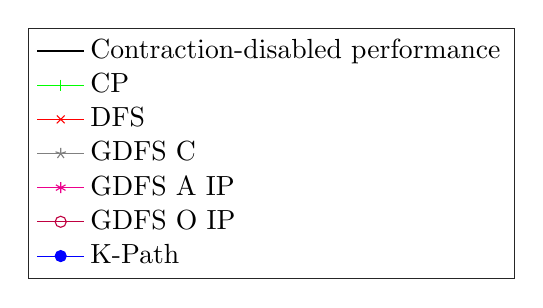
\begin{tikzpicture} 
    \begin{axis}[%
    hide axis,
    xmin=10,
    xmax=50,
    ymin=0,
    ymax=0.4,
    legend style={draw=white!15!black,legend cell align=left}
    ]
	\addlegendimage{black}
    \addlegendentry{Contraction-disabled performance}; 
     
    \addlegendimage{green, mark=+}
    \addlegendentry{CP};
    
    \addlegendimage{red, mark=x}
    \addlegendentry{DFS};
    
    \addlegendimage{gray, mark=star}
    \addlegendentry{GDFS C};
    
    \addlegendimage{magenta, mark=asterisk}
    \addlegendentry{GDFS A IP};
    
    \addlegendimage{purple, mark=o}
    \addlegendentry{GDFS O IP};
    
    \addlegendimage{blue, mark=*}
    \addlegendentry{K-Path};
    
    \end{axis}
\end{tikzpicture}

\end{subfigure}

\caption{Performance of our algorithm with \textbf{ZeroDomain} pruning using \textbf{`M-filtering'} filtering relative to the performance of the algorithm without pruning. We avoid unnecessarily long paths, do not perform contraction and use the degree-based target graph vertex ordering. Data points above the black reference line denote that the pruning method introduces more delay, and data points below the reference line denote that the pruning method saves time. Note the logarithmic y-axis.}	
\label{fig:test}
\end{figure}

\begin{figure}
\begin{subfigure}{.5\linewidth}
\centering

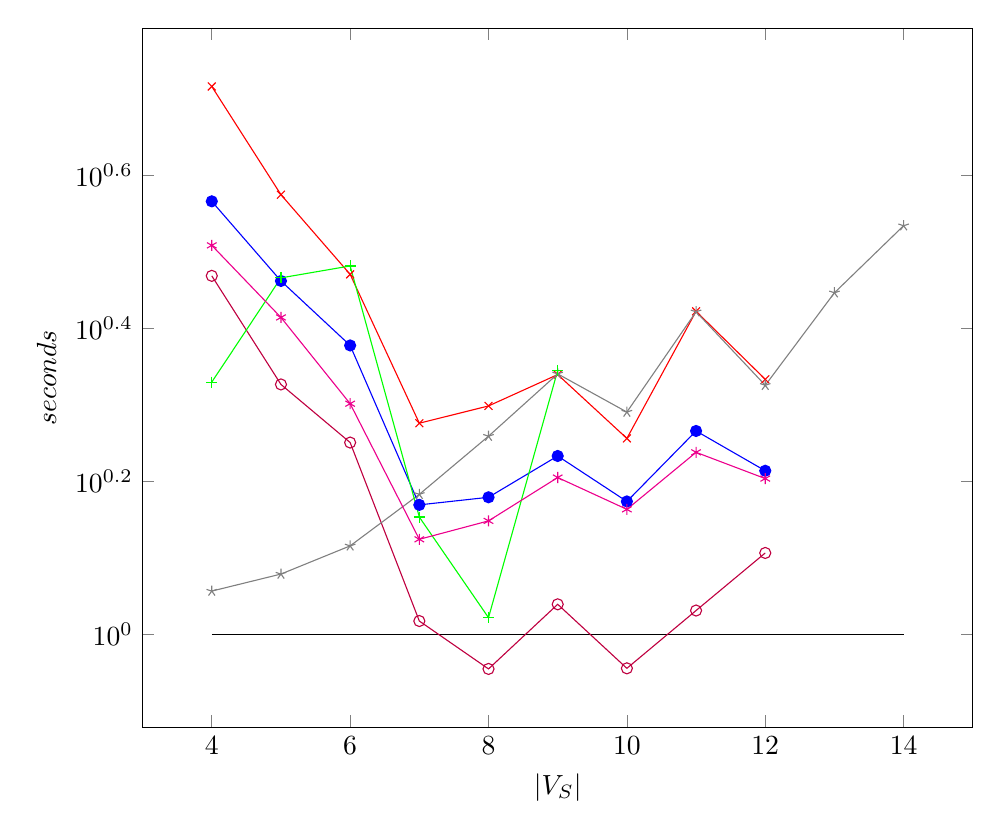
\begin{tikzpicture}
        \begin{axis}[
        xlabel=$|V_S|$,
        ylabel=$seconds$,
        ymode=log,
        legend style={at={(0.9,0.1)},anchor=south east},
        width=\textwidth,
		y tick label style={/pgf/number format/sci},
    ]
\addplot [mark=none, black] plot coordinates {
        (4,1) (14, 1)};

    
   

\addplot[
        mark=x,
        red,
    ] plot coordinates {
        (4,5.202946551261944)
        (5,3.756162046192574)
        (6,2.9549254023879072)
        (7,1.8872742557474473)
        (8,1.9880582223277101)
        (9,2.1847812854733193)
        (10,1.8028559351037163)
        (11,2.6436531391416507)
        (12,2.1539273359082483)
};
%    \addlegendentry{DFS}


\addplot[
        mark=o,
        purple,
    ] plot coordinates {
        (4,2.9414858115997387)
        (5,2.120863031356877)
        (6,1.7804930224229873)
        (7,1.0400701807728874)
        (8,0.9003554054490217)
        (9,1.0937936596519373)
        (10,0.9019831415298204)
        (11,1.0734764108654673)
        (12,1.2767276824510232)
};
%    \addlegendentry{GDFS O IP}


\addplot[
        mark=star,
        gray,
    ] plot coordinates {
        (4,1.1382355278673217)
        (5,1.198063456290179)
        (6,1.3042425098741526)
        (7,1.5233183009320665)
        (8,1.8148828000886499)
        (9,2.189451318312936)
        (10,1.9518249758925157)
        (11,2.639768817120566)
        (12,2.1154918845964863)
        (13,2.7952098947822313)
        (14,3.4210781907374623)
};
%    \addlegendentry{GDFS C}


\addplot[
        mark=*,
        blue,
    ] plot coordinates {
        (4,3.6819210072894446)
        (5,2.896400619358773)
        (6,2.3852188316658136)
        (7,1.4756755823523737)
        (8,1.5098085945063882)
        (9,1.7097753943529064)
        (10,1.490937989140139)
        (11,1.8438583447137513)
        (12,1.635315159939935)
};
%    \addlegendentry{K-Path}


\addplot[
        mark=+,
        green,
    ] plot coordinates {
        (4,2.1359021980392736)
        (5,2.923428609692478)
        (6,3.0304568963312812)
        (7,1.4225695726266137)
        (8,1.0506565420981449)
        (9,2.212314905046649)
};
%    \addlegendentry{CP}


\addplot[
        mark=asterisk,
        magenta,
    ] plot coordinates {
        (4,3.2242822734185275)
        (5,2.5950345747500103)
        (6,2.0014242504647624)
        (7,1.3303134982815363)
        (8,1.4062726411755775)
        (9,1.6024494454371436)
        (10,1.4559250035524376)
        (11,1.7288683972843149)
        (12,1.5973164420401704)
};
%    \addlegendentry{GDFS A IP}


    \end{axis}
    \end{tikzpicture}


\caption{serial}
\label{fig:sub1}
\end{subfigure}%
\begin{subfigure}{.5\linewidth}
\centering

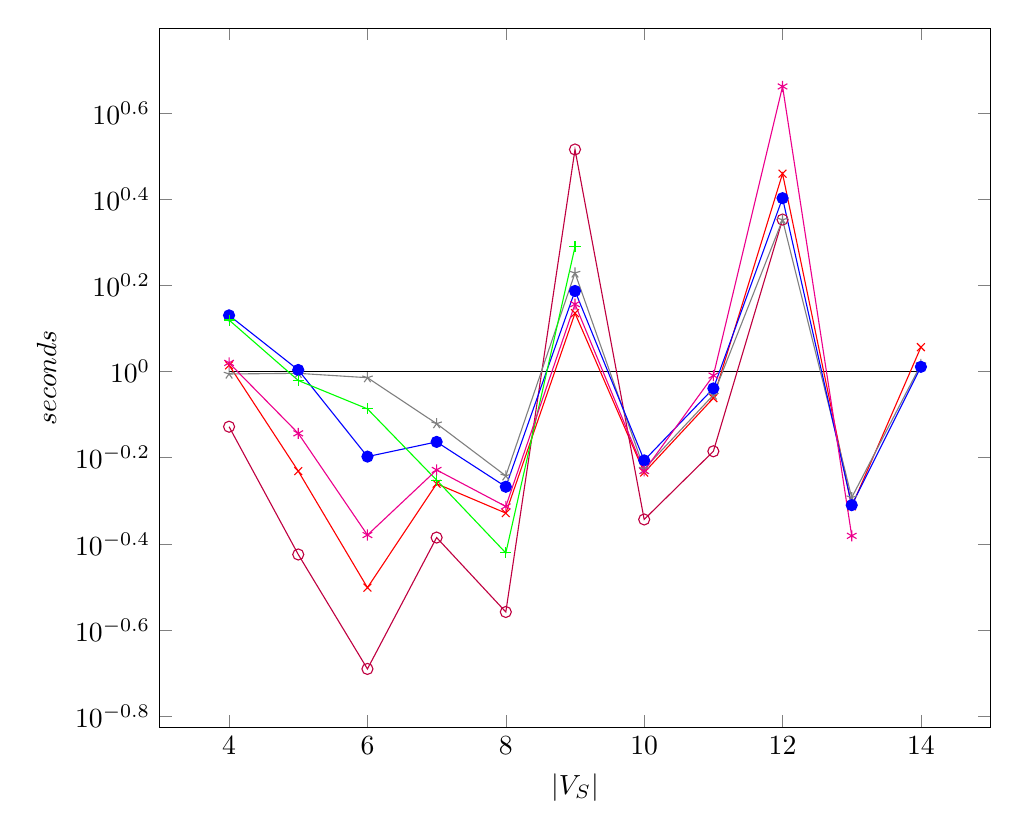
\begin{tikzpicture}
    \begin{axis}[
        xlabel=$|V_S|$,
        ylabel=$seconds$,
        ymode=log,
        legend style={at={(0.9,0.1)},anchor=south east},
        width=\textwidth,
		y tick label style={/pgf/number format/sci},
    ]
\addplot [mark=none, black] plot coordinates {
        (4,1) (14, 1)};



\addplot[
        mark=x,
        red,
    ] plot coordinates {
        (4,1.0341963936340537)
        (5,0.5872212498317262)
        (6,0.3150252343592421)
        (7,0.5489328540502025)
        (8,0.4691563660507788)
        (9,1.3659267214920254)
        (10,0.5829158055427053)
        (11,0.8675410228213514)
        (12,2.8804215346851567)
        (13,0.48622042850802205)
        (14,1.139249103225921)
};
%    \addlegendentry{DFS}


\addplot[
        mark=o,
        purple,
    ] plot coordinates {
        (4,0.7446160731342548)
        (5,0.3760872484757529)
        (6,0.20395691063619348)
        (7,0.4116723120141347)
        (8,0.2765761366043523)
        (9,3.277702486377702)
        (10,0.45345557621451693)
        (11,0.6529131347050375)
        (12,2.253102642969394)
};
%    \addlegendentry{GDFS O IP}


\addplot[
        mark=star,
        gray,
    ] plot coordinates {
        (4,0.986998285923268)
        (5,0.990456016904658)
        (6,0.9676159305638337)
        (7,0.7569661999435013)
        (8,0.5726394480903727)
        (9,1.6935978244098564)
        (10,0.5939935948858152)
        (11,0.8819548932880411)
        (12,2.250262287942807)
        (13,0.5098016055539938)
        (14,1.0382537813550197)
};
%    \addlegendentry{GDFS C}


\addplot[
        mark=*,
        blue,
    ] plot coordinates {
        (4,1.350280192589271)
        (5,1.0083990021448497)
        (6,0.6346349881535795)
        (7,0.6865130883699138)
        (8,0.5401179927275145)
        (9,1.5384974483498595)
        (10,0.6218905966067542)
        (11,0.9136191743894921)
        (12,2.5263424220943915)
        (13,0.4895304853304312)
        (14,1.025493765853684)
};
%    \addlegendentry{K-Path}


\addplot[
        mark=+,
        green,
    ] plot coordinates {
        (4,1.316795353041837)
        (5,0.9532402532500417)
        (6,0.8191487199612747)
        (7,0.5596281163603946)
        (8,0.3792225987672416)
        (9,1.9471981919246635)
};
%    \addlegendentry{CP}


\addplot[
        mark=asterisk,
        magenta,
    ] plot coordinates {
        (4,1.0472612442074125)
        (5,0.718669879592718)
        (6,0.4172863346749811)
        (7,0.5909828175058394)
        (8,0.48615922809785606)
        (9,1.4337866356743774)
        (10,0.5877303758542455)
        (11,0.9788108288373746)
        (12,4.589963118304846)
        (13,0.4155118413601153)
};
%    \addlegendentry{GDFS A IP}

	
	
    \end{axis}
    \end{tikzpicture}

\caption{cached}
\label{fig:sub2}
\end{subfigure}\\[1ex]
\begin{subfigure}{0.5\linewidth}
\centering

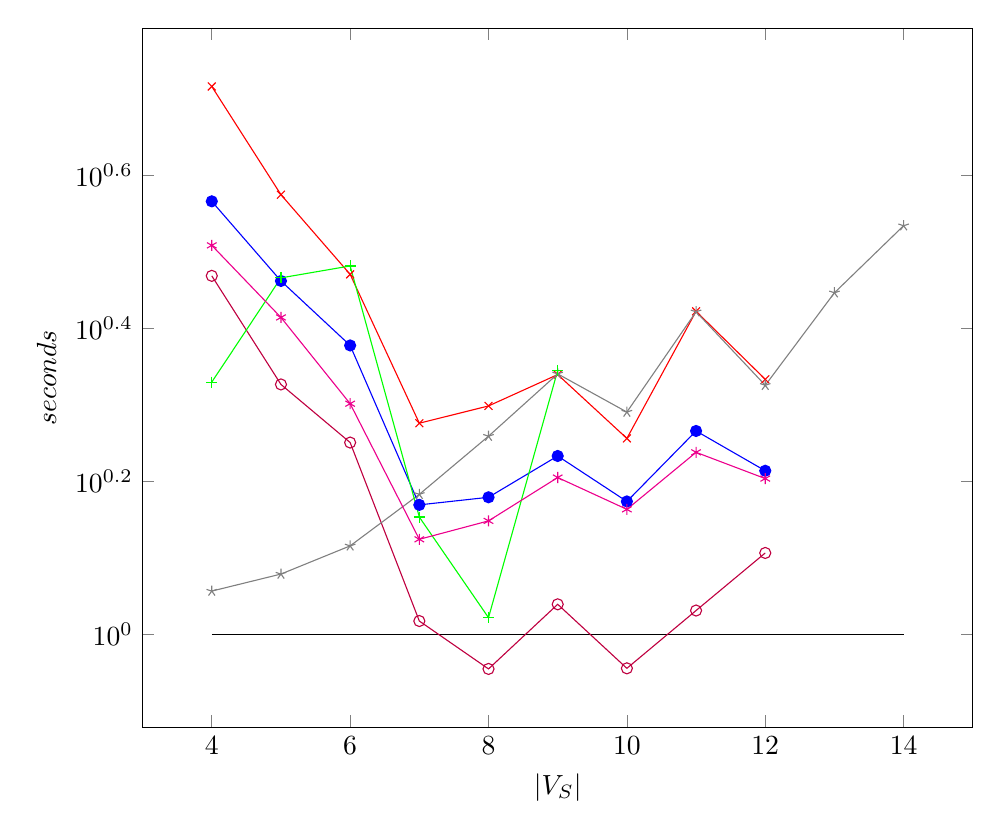
\begin{tikzpicture}
    \begin{axis}[
        xlabel=$|V_S|$,
        ylabel=$seconds$,
        ymode=log,
        legend style={at={(0.9,0.1)},anchor=south east},
        width=\textwidth,
		y tick label style={/pgf/number format/sci},
    ]
\addplot [mark=none, black] plot coordinates {
        (4,1) (14, 1)};



\addplot[
        mark=x,
        red,
    ] plot coordinates {
        (4,5.202946551261944)
        (5,3.756162046192574)
        (6,2.9549254023879072)
        (7,1.8872742557474473)
        (8,1.9880582223277101)
        (9,2.1847812854733193)
        (10,1.8028559351037163)
        (11,2.6436531391416507)
        (12,2.1539273359082483)
};
%    \addlegendentry{DFS}


\addplot[
        mark=o,
        purple,
    ] plot coordinates {
        (4,2.9414858115997387)
        (5,2.120863031356877)
        (6,1.7804930224229873)
        (7,1.0400701807728874)
        (8,0.9003554054490217)
        (9,1.0937936596519373)
        (10,0.9019831415298204)
        (11,1.0734764108654673)
        (12,1.2767276824510232)
};
%    \addlegendentry{GDFS O IP}


\addplot[
        mark=star,
        gray,
    ] plot coordinates {
        (4,1.1382355278673217)
        (5,1.198063456290179)
        (6,1.3042425098741526)
        (7,1.5233183009320665)
        (8,1.8148828000886499)
        (9,2.189451318312936)
        (10,1.9518249758925157)
        (11,2.639768817120566)
        (12,2.1154918845964863)
        (13,2.7952098947822313)
        (14,3.4210781907374623)
};
%    \addlegendentry{GDFS C}


\addplot[
        mark=*,
        blue,
    ] plot coordinates {
        (4,3.6819210072894446)
        (5,2.896400619358773)
        (6,2.3852188316658136)
        (7,1.4756755823523737)
        (8,1.5098085945063882)
        (9,1.7097753943529064)
        (10,1.490937989140139)
        (11,1.8438583447137513)
        (12,1.635315159939935)
};
%    \addlegendentry{K-Path}


\addplot[
        mark=+,
        green,
    ] plot coordinates {
        (4,2.1359021980392736)
        (5,2.923428609692478)
        (6,3.0304568963312812)
        (7,1.4225695726266137)
        (8,1.0506565420981449)
        (9,2.212314905046649)
};
%    \addlegendentry{CP}


\addplot[
        mark=asterisk,
        magenta,
    ] plot coordinates {
        (4,3.2242822734185275)
        (5,2.5950345747500103)
        (6,2.0014242504647624)
        (7,1.3303134982815363)
        (8,1.4062726411755775)
        (9,1.6024494454371436)
        (10,1.4559250035524376)
        (11,1.7288683972843149)
        (12,1.5973164420401704)
};
%    \addlegendentry{GDFS A IP}

	
    \end{axis}
    \end{tikzpicture}

\caption{parallel}
\label{fig:sub3}
\end{subfigure}
\begin{subfigure} {0.5\linewidth}
\centering

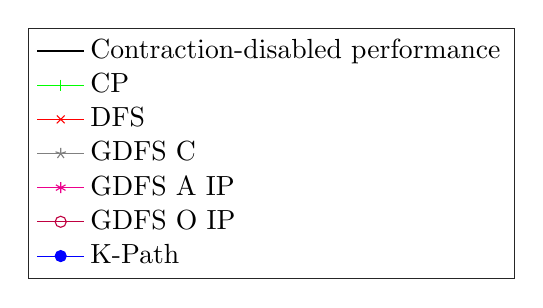
\begin{tikzpicture} 
    \begin{axis}[%
    hide axis,
    xmin=10,
    xmax=50,
    ymin=0,
    ymax=0.4,
    legend style={draw=white!15!black,legend cell align=left}
    ]
	\addlegendimage{black}
    \addlegendentry{Contraction-disabled performance}; 
     
    \addlegendimage{green, mark=+}
    \addlegendentry{CP};
    
    \addlegendimage{red, mark=x}
    \addlegendentry{DFS};
    
    \addlegendimage{gray, mark=star}
    \addlegendentry{GDFS C};
    
    \addlegendimage{magenta, mark=asterisk}
    \addlegendentry{GDFS A IP};
    
    \addlegendimage{purple, mark=o}
    \addlegendentry{GDFS O IP};
    
    \addlegendimage{blue, mark=*}
    \addlegendentry{K-Path};
    
    \end{axis}
\end{tikzpicture}

\end{subfigure}

\caption{Performance of our algorithm with \textbf{ZeroDomain} pruning using \textbf{`N-Filtering'} filtering relative to the performance of the algorithm without pruning. We avoid unnecessarily long paths, do not perform contraction and use the degree-based target graph vertex ordering. Data points above the black reference line denote that the pruning method introduces more delay, and data points below the reference line denote that the pruning method saves time. Note the logarithmic y-axis.}	
\label{fig:test}
\end{figure}

\begin{figure}
\begin{subfigure}{.5\linewidth}
\centering

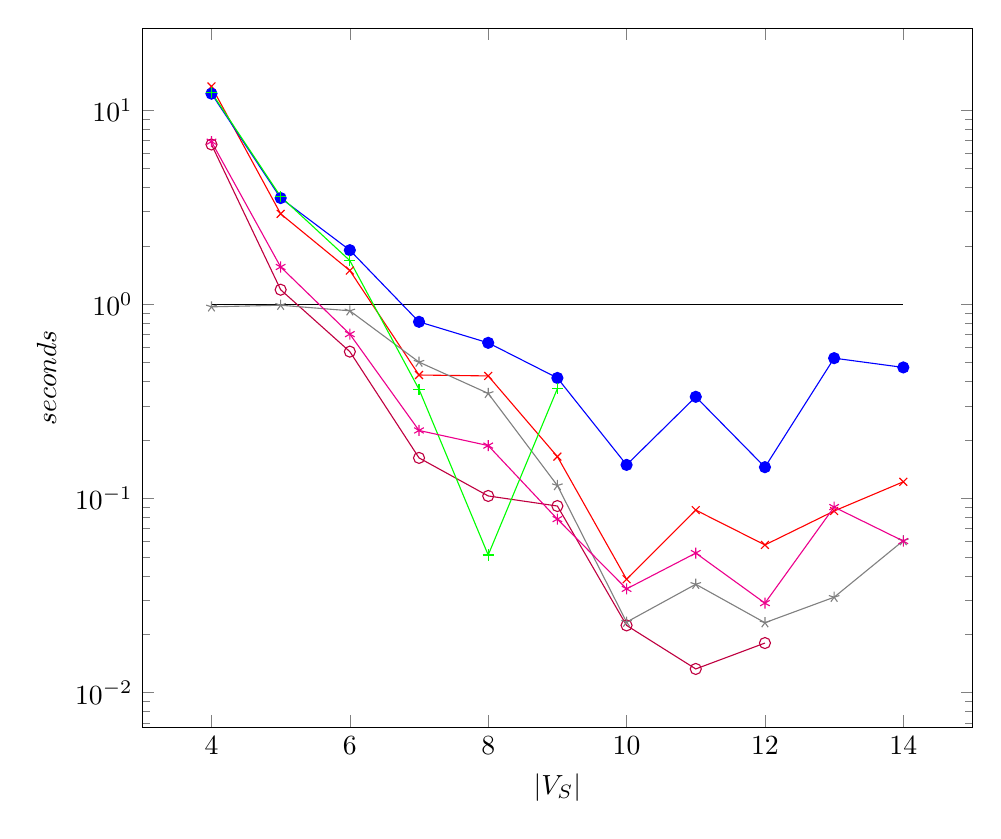
\begin{tikzpicture}
    \begin{axis}[
        xlabel=$|V_S|$,
        ylabel=$seconds$,
        ymode=log,
        legend style={at={(0.9,0.1)},anchor=south east},
        width=\textwidth,
		y tick label style={/pgf/number format/sci},
    ]
\addplot [mark=none, black] plot coordinates {
        (4,1) (14, 1)};

    
	

\addplot[
        mark=x,
        red,
    ] plot coordinates {
        (4,13.228536748772864)
        (5,2.923043265236232)
        (6,1.4918465046685692)
        (7,0.43251422608381307)
        (8,0.4278138461953538)
        (9,0.1643974532055621)
        (10,0.0384235218883735)
        (11,0.08720339702951019)
        (12,0.05769871433439522)
        (13,0.08626318052038495)
        (14,0.12196687793734029)
};
%    \addlegendentry{DFS}


\addplot[
        mark=o,
        purple,
    ] plot coordinates {
        (4,6.652084765296219)
        (5,1.1887666847267304)
        (6,0.5706904469839822)
        (7,0.1619203743990465)
        (8,0.10311284594841497)
        (9,0.09148726872328639)
        (10,0.02222929883828284)
        (11,0.013264269229998682)
        (12,0.01803108077997606)
};
%    \addlegendentry{GDFS O IP}


\addplot[
        mark=star,
        gray,
    ] plot coordinates {
        (4,0.9704520516781957)
        (5,0.9891315449448252)
        (6,0.9259991321183858)
        (7,0.5041146272686665)
        (8,0.34789464456875185)
        (9,0.11668758068736773)
        (10,0.023108258037857765)
        (11,0.03619415549870497)
        (12,0.022948727466520213)
        (13,0.031049777535341994)
        (14,0.06069360971979865)
};
%    \addlegendentry{GDFS C}


\addplot[
        mark=*,
        blue,
    ] plot coordinates {
        (4,12.149621156018027)
        (5,3.524039042210963)
        (6,1.9000540945545796)
        (7,0.8124353858557827)
        (8,0.6333558749485183)
        (9,0.4176331133841372)
        (10,0.1490144308922331)
        (11,0.33404804566046264)
        (12,0.14504260141405623)
        (13,0.5281107544448288)
        (14,0.4731679498288802)
};
%    \addlegendentry{K-Path}


\addplot[
        mark=+,
        green,
    ] plot coordinates {
        (4,12.32026911652997)
        (5,3.58755573944772)
        (6,1.6790110096274846)
        (7,0.36496009660452833)
        (8,0.05120848928373445)
        (9,0.3680142027878651)
};
%    \addlegendentry{CP}


\addplot[
        mark=asterisk,
        magenta,
    ] plot coordinates {
        (4,6.876029334720606)
        (5,1.556841256929411)
        (6,0.7022607700874779)
        (7,0.22412843275278505)
        (8,0.18733394302820017)
        (9,0.07837119253519409)
        (10,0.03427027564684937)
        (11,0.05237617390308613)
        (12,0.028947697493439506)
        (13,0.09038890815957701)
        (14,0.0604047187048502)
};
%    \addlegendentry{GDFS A IP}
  
   
   
   

    \end{axis}
    \end{tikzpicture}


\caption{serial}
\label{fig:sub1}
\end{subfigure}%
\begin{subfigure}{.5\linewidth}
\centering

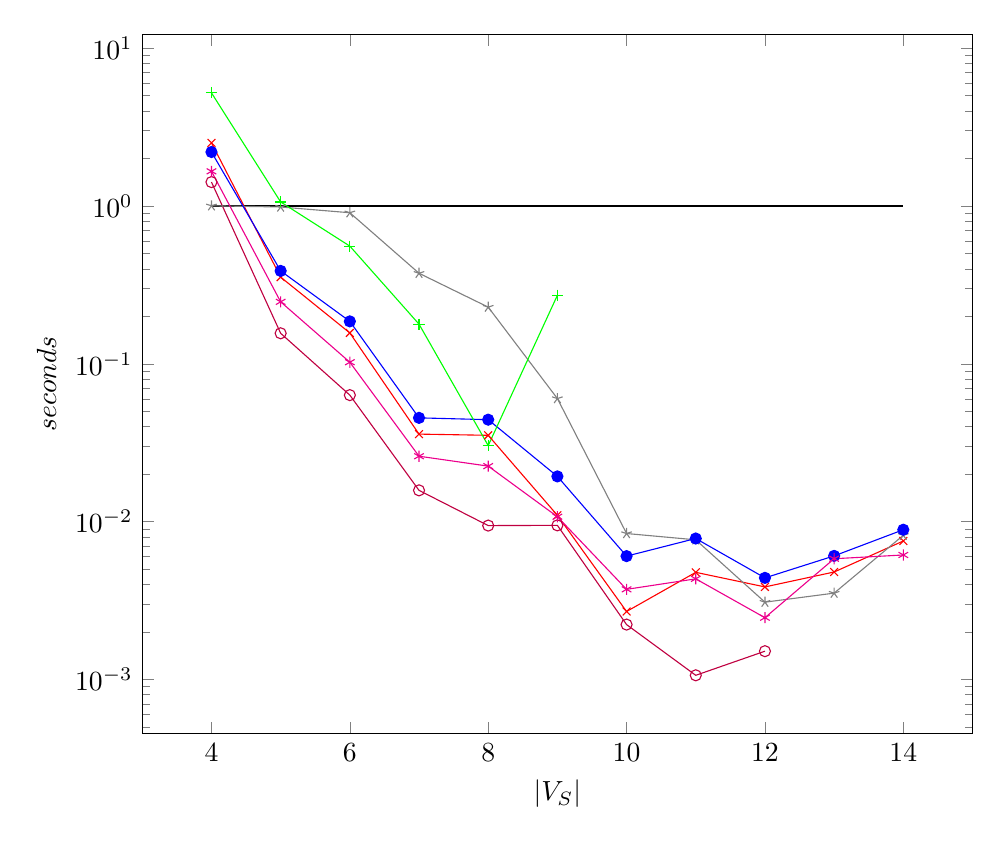
\begin{tikzpicture}
    \begin{axis}[
        xlabel=$|V_S|$,
        ylabel=$seconds$,
        ymode=log,
        legend style={at={(0.9,0.1)},anchor=south east},
        width=\textwidth,
		y tick label style={/pgf/number format/sci},
    ]
\addplot [mark=none, black] plot coordinates {
        (4,1) (14, 1)};



\addplot[
        mark=x,
        red,
    ] plot coordinates {
        (4,2.5098178926779067)
        (5,0.3542854427484565)
        (6,0.15689010926635982)
        (7,0.035853449977087615)
        (8,0.03523223883158477)
        (9,0.010964699575333747)
        (10,0.0026948377810716018)
        (11,0.0047722023475749165)
        (12,0.003857850717237876)
        (13,0.0047953458790988)
        (14,0.007540380523948009)
};
%    \addlegendentry{DFS}


\addplot[
        mark=o,
        purple,
    ] plot coordinates {
        (4,1.4173101034075382)
        (5,0.1560990152619649)
        (6,0.06332634097438505)
        (7,0.0157805848059952)
        (8,0.009438491623514178)
        (9,0.009468907924155778)
        (10,0.002226287610086919)
        (11,0.001062190759533732)
        (12,0.0015102350651220453)
};
%    \addlegendentry{GDFS O IP}


\addplot[
        mark=star,
        gray,
    ] plot coordinates {
        (4,1.002529859429505)
        (5,0.9854105159518796)
        (6,0.906087246903251)
        (7,0.3747194523117736)
        (8,0.22865139116910282)
        (9,0.060236499046310454)
        (10,0.00840605207241163)
        (11,0.0076697916371780694)
        (12,0.003087366357886867)
        (13,0.003523082302813507)
        (14,0.008191107040264711)
};
%    \addlegendentry{GDFS C}


\addplot[
        mark=*,
        blue,
    ] plot coordinates {
        (4,2.1976489735425813)
        (5,0.3879928825633856)
        (6,0.18575151663949174)
        (7,0.0454443516390044)
        (8,0.044259974145741565)
        (9,0.01934413411554503)
        (10,0.006044262197985706)
        (11,0.007817157760072191)
        (12,0.004400728544806665)
        (13,0.0060658785631791945)
        (14,0.008884903299891778)
};
%    \addlegendentry{K-Path}


\addplot[
        mark=+,
        green,
    ] plot coordinates {
        (4,5.210336306845926)
        (5,1.0605278688734023)
        (6,0.5567531798646309)
        (7,0.17832988212555723)
        (8,0.03032795503714869)
        (9,0.2717523415218701)
};
%    \addlegendentry{CP}


\addplot[
        mark=asterisk,
        magenta,
    ] plot coordinates {
        (4,1.6585184570290825)
        (5,0.24696367603814495)
        (6,0.102320267871855)
        (7,0.025963378720697206)
        (8,0.02247569274863903)
        (9,0.010741035240163122)
        (10,0.003723269579006816)
        (11,0.004340017423267284)
        (12,0.0024617244953977213)
        (13,0.0058187731897781925)
        (14,0.006146499125306626)
};
%    \addlegendentry{GDFS A IP}

	
    \end{axis}
    \end{tikzpicture}

\caption{cached}
\label{fig:sub2}
\end{subfigure}\\[1ex]
\begin{subfigure}{0.5\linewidth}
\centering

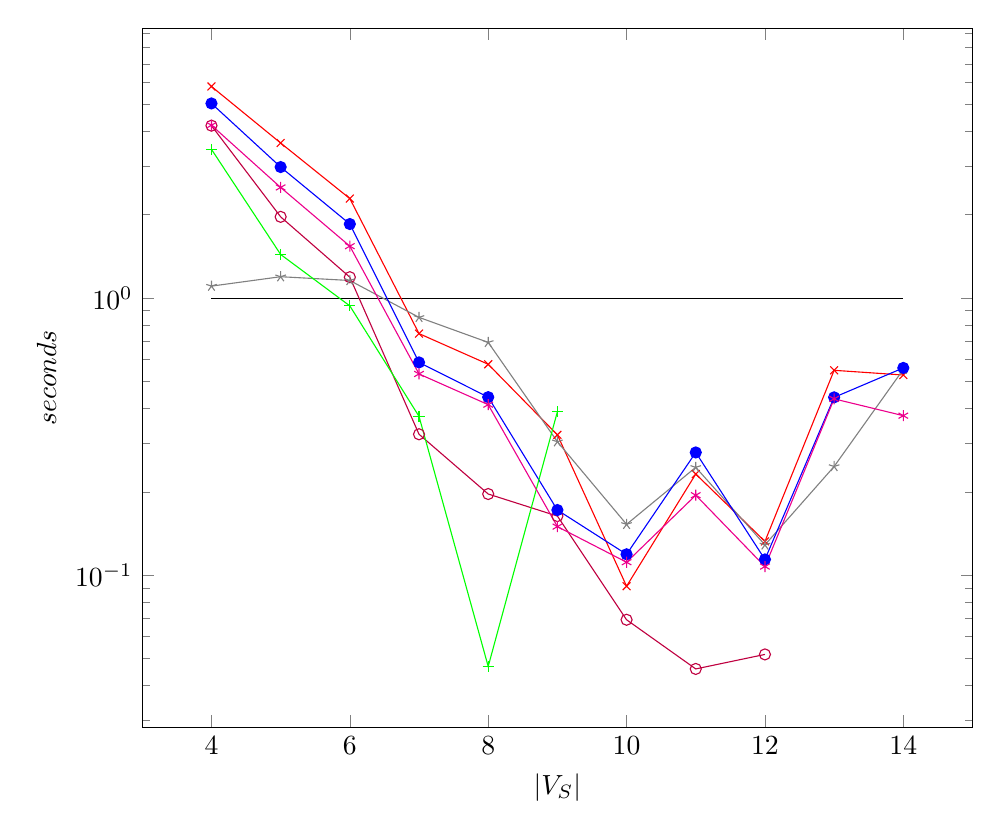
\begin{tikzpicture}
    \begin{axis}[
        xlabel=$|V_S|$,
        ylabel=$seconds$,
        ymode=log,
        legend style={at={(0.9,0.1)},anchor=south east},
        width=\textwidth,
		y tick label style={/pgf/number format/sci},
    ]
\addplot [mark=none, black] plot coordinates {
        (4,1) (14, 1)};



\addplot[
        mark=x,
        red,
    ] plot coordinates {
        (4,5.798792679850153)
        (5,3.6257004403518205)
        (6,2.285202142417693)
        (7,0.7445129848838659)
        (8,0.5770188169893984)
        (9,0.3210938826132116)
        (10,0.09131787739629149)
        (11,0.23183733254071692)
        (12,0.13250978599133645)
        (13,0.5487572087616573)
        (14,0.5277236677256409)
};
%    \addlegendentry{DFS}


\addplot[
        mark=o,
        purple,
    ] plot coordinates {
        (4,4.1869563644643)
        (5,1.963563805539359)
        (6,1.1893882290176945)
        (7,0.3225915596294)
        (8,0.196417660886969)
        (9,0.1635088016201688)
        (10,0.06910862435318588)
        (11,0.045930260406800816)
        (12,0.0518105433910061)
};
%    \addlegendentry{GDFS O IP}


\addplot[
        mark=star,
        gray,
    ] plot coordinates {
        (4,1.1043656381381906)
        (5,1.1941146142677403)
        (6,1.1571769969713963)
        (7,0.8519147110949141)
        (8,0.6919890069549386)
        (9,0.30329744854481366)
        (10,0.15267006969696184)
        (11,0.2451122958148758)
        (12,0.12868565849738745)
        (13,0.2468665194487868)
        (14,0.5529525262522433)
};
%    \addlegendentry{GDFS C}


\addplot[
        mark=*,
        blue,
    ] plot coordinates {
        (4,5.036262260510419)
        (5,2.969188933770786)
        (6,1.8496830497872034)
        (7,0.5859718273323613)
        (8,0.43912493395440744)
        (9,0.17191408110115602)
        (10,0.11902810316960899)
        (11,0.2773735237523154)
        (12,0.114049211518233)
        (13,0.438365362697428)
        (14,0.5597451487697097)
};
%    \addlegendentry{K-Path}


\addplot[
        mark=+,
        green,
    ] plot coordinates {
        (4,3.4404078593966663)
        (5,1.4365332891311595)
        (6,0.9370666124380356)
        (7,0.37433319924673136)
        (8,0.04688253357281991)
        (9,0.38910890933793285)
};
%    \addlegendentry{CP}


\addplot[
        mark=asterisk,
        magenta,
    ] plot coordinates {
        (4,4.202135993006676)
        (5,2.5066991227985915)
        (6,1.5392306053079454)
        (7,0.5323918363219251)
        (8,0.41254854061922086)
        (9,0.14979269284608565)
        (10,0.11144241399443222)
        (11,0.1944784771207959)
        (12,0.10750387177004295)
        (13,0.43288906698477536)
        (14,0.37647551651848066)
};
%    \addlegendentry{GDFS A IP}

	
    \end{axis}
    \end{tikzpicture}

\caption{parallel}
\label{fig:sub3}
\end{subfigure}
\begin{subfigure} {0.5\linewidth}
\centering

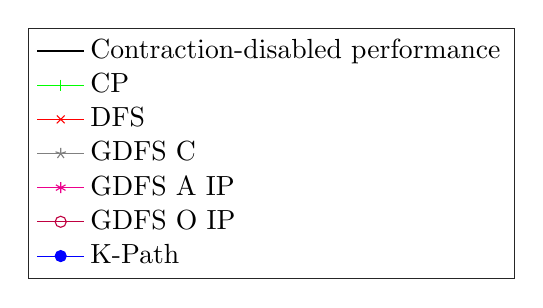
\begin{tikzpicture} 
    \begin{axis}[%
    hide axis,
    xmin=10,
    xmax=50,
    ymin=0,
    ymax=0.4,
    legend style={draw=white!15!black,legend cell align=left}
    ]
	\addlegendimage{black}
    \addlegendentry{Contraction-disabled performance}; 
     
    \addlegendimage{green, mark=+}
    \addlegendentry{CP};
    
    \addlegendimage{red, mark=x}
    \addlegendentry{DFS};
    
    \addlegendimage{gray, mark=star}
    \addlegendentry{GDFS C};
    
    \addlegendimage{magenta, mark=asterisk}
    \addlegendentry{GDFS A IP};
    
    \addlegendimage{purple, mark=o}
    \addlegendentry{GDFS O IP};
    
    \addlegendimage{blue, mark=*}
    \addlegendentry{K-Path};
    
    \end{axis}
\end{tikzpicture}

\end{subfigure}

\caption{Performance of our algorithm with \textbf{AllDifferent} pruning using \textbf{`Labels and neighbours'} filtering relative to the performance of the algorithm without pruning. We avoid unnecessarily long paths, do not perform contraction and use the degree-based target graph vertex ordering. Data points above the black reference line denote that the pruning method introduces more delay, and data points below the reference line denote that the pruning method saves time. Note the logarithmic y-axis.}	
\label{fig:test}
\end{figure}

\begin{figure}
\begin{subfigure}{.5\linewidth}
\centering

\begin{tikzpicture}
    \begin{axis}[
        xlabel=$|V_S|$,
        ylabel=$seconds$,
        ymode=log,
        legend style={at={(0.9,0.1)},anchor=south east},
        width=\textwidth,
		y tick label style={/pgf/number format/sci},
    ]
\addplot [mark=none, black] plot coordinates {
        (4,1) (14, 1)};

    
   

\addplot[
        mark=x,
        red,
    ] plot coordinates {
        (4,1.0186997833347926)
        (5,1.0232045351532169)
        (6,0.9983077611450746)
        (7,0.9907049947363294)
        (8,0.9986106752415018)
        (9,0.990947997808037)
        (10,0.9833582387420912)
        (11,0.9932844129587108)
        (12,1.0103133629860612)
        (13,0.8895477690842722)
        (14,1.005905267592158)
};
%    \addlegendentry{DFS}


\addplot[
        mark=o,
        purple,
    ] plot coordinates {
        (4,0.9894734471098923)
        (5,0.9968820127769855)
        (6,0.9873225419658352)
        (7,0.9858166681275962)
        (8,0.9904807801930379)
        (9,0.996328709955975)
        (10,0.9809044726735501)
        (11,1.0231407177222254)
        (12,1.0305198945131373)
};
%    \addlegendentry{GDFS O IP}


\addplot[
        mark=star,
        gray,
    ] plot coordinates {
        (4,0.9951732111609184)
        (5,1.005781000751052)
        (6,0.9751302373376524)
        (7,0.9914699309037306)
        (8,1.011362037912515)
        (9,0.9843712362591021)
        (10,0.969402089834849)
        (11,1.0237476067658449)
        (12,1.137294643132325)
        (13,0.9744371513907365)
        (14,0.9802787976693997)
};
%    \addlegendentry{GDFS C}


\addplot[
        mark=*,
        blue,
    ] plot coordinates {
        (4,1.0092933808186613)
        (5,0.7972700999022878)
        (6,0.3874509873372779)
        (7,0.12257854741680918)
        (8,0.11535787568739275)
        (9,0.05517912995992491)
        (10,0.027274471216057083)
        (11,0.09778018796630517)
        (12,0.030614788275003413)
        (13,0.03405177172923535)
        (14,0.17825871037578678)
};
%    \addlegendentry{K-Path}


\addplot[
        mark=+,
        green,
    ] plot coordinates {
        (4,1.0028356859109526)
        (5,0.9904361969575739)
        (6,0.9923987001325429)
        (7,1.0046817332100164)
        (8,0.9858188647918942)
        (9,1.0225063689622522)
};
%    \addlegendentry{CP}


\addplot[
        mark=asterisk,
        magenta,
    ] plot coordinates {
        (4,0.9976349962184932)
        (5,1.0073844165930093)
        (6,0.9981453884688307)
        (7,0.9876792768127225)
        (8,1.0133814377011994)
        (9,0.9520147690376894)
        (10,0.9790339992527488)
        (11,0.9908681483629362)
        (12,1.039543646663335)
        (13,0.9354622696539593)
};
%    \addlegendentry{GDFS A IP}


    \end{axis}
    \end{tikzpicture}


\caption{serial}
\label{fig:sub1}
\end{subfigure}%
\begin{subfigure}{.5\linewidth}
\centering

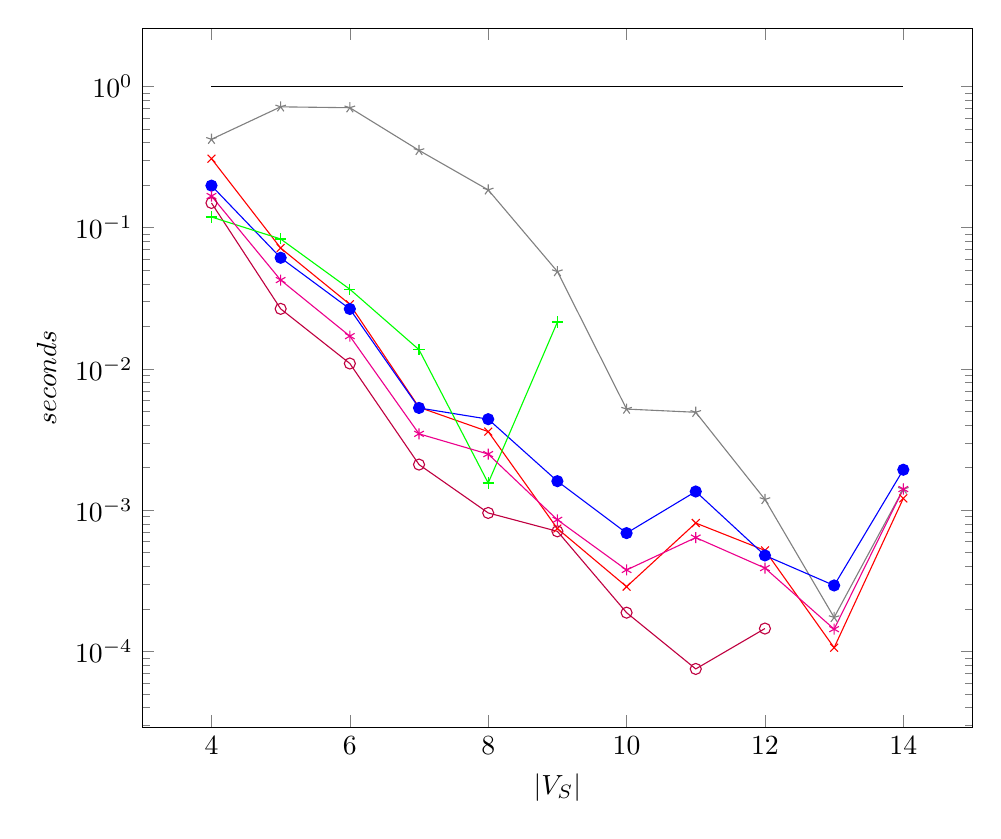
\begin{tikzpicture}
    \begin{axis}[
        xlabel=$|V_S|$,
        ylabel=$seconds$,
        ymode=log,
        legend style={at={(0.9,0.1)},anchor=south east},
        width=\textwidth,
		y tick label style={/pgf/number format/sci},
    ]
\addplot [mark=none, black] plot coordinates {
        (4,1) (14, 1)};


	

\addplot[
        mark=x,
        red,
    ] plot coordinates {
        (4,0.3083735334423767)
        (5,0.0717983121165574)
        (6,0.02867174161124386)
        (7,0.005353932759145197)
        (8,0.0036018766107605016)
        (9,7.415681550873021E-4)
        (10,2.875045828804046E-4)
        (11,8.113057744684182E-4)
        (12,5.194226380311751E-4)
        (13,1.0634101119189054E-4)
        (14,0.0012129348920926208)
};
%    \addlegendentry{DFS}


\addplot[
        mark=o,
        purple,
    ] plot coordinates {
        (4,0.14979438676735934)
        (5,0.026646145040194358)
        (6,0.010934376147201053)
        (7,0.0021043263511895116)
        (8,9.565212575048943E-4)
        (9,7.087506618627115E-4)
        (10,1.8824424486718616E-4)
        (11,7.522826832084828E-5)
        (12,1.452779418016359E-4)
};
%    \addlegendentry{GDFS O IP}


\addplot[
        mark=star,
        gray,
    ] plot coordinates {
        (4,0.42295684080525053)
        (5,0.7175652095808638)
        (6,0.7072294111057362)
        (7,0.3528461610206276)
        (8,0.1853565026591184)
        (9,0.04895326827559776)
        (10,0.00520061691970819)
        (11,0.004936257731941951)
        (12,0.001192029881315615)
        (13,1.741539188091501E-4)
        (14,0.0014103432783372227)
};
%    \addlegendentry{GDFS C}


\addplot[
        mark=*,
        blue,
    ] plot coordinates {
        (4,0.19863010172526796)
        (5,0.06127991045420755)
        (6,0.02659926027389259)
        (7,0.005297029257396946)
        (8,0.004410971673992958)
        (9,0.0016052971971944885)
        (10,6.884416663917037E-4)
        (11,0.0013566163358025296)
        (12,4.784200055767407E-4)
        (13,2.932097067133155E-4)
        (14,0.0019350025642613788)
};
%    \addlegendentry{K-Path}


\addplot[
        mark=+,
        green,
    ] plot coordinates {
        (4,0.11914885358071148)
        (5,0.08325890354708809)
        (6,0.03669565157098442)
        (7,0.013693561308514623)
        (8,0.0015581760794368682)
        (9,0.021493389120216477)
};
%    \addlegendentry{CP}


\addplot[
        mark=asterisk,
        magenta,
    ] plot coordinates {
        (4,0.167629941635991)
        (5,0.04261429975714803)
        (6,0.01708358998028725)
        (7,0.0034731132709504564)
        (8,0.0024963114206875137)
        (9,8.552890640062261E-4)
        (10,3.776131025451379E-4)
        (11,6.400771612525835E-4)
        (12,3.8951787719665454E-4)
        (13,1.4388024718858805E-4)
        (14,0.0014124109249871175)
};
%    \addlegendentry{GDFS A IP}

	
    \end{axis}
    \end{tikzpicture}

\caption{cached}
\label{fig:sub2}
\end{subfigure}\\[1ex]
\begin{subfigure}{0.5\linewidth}
\centering

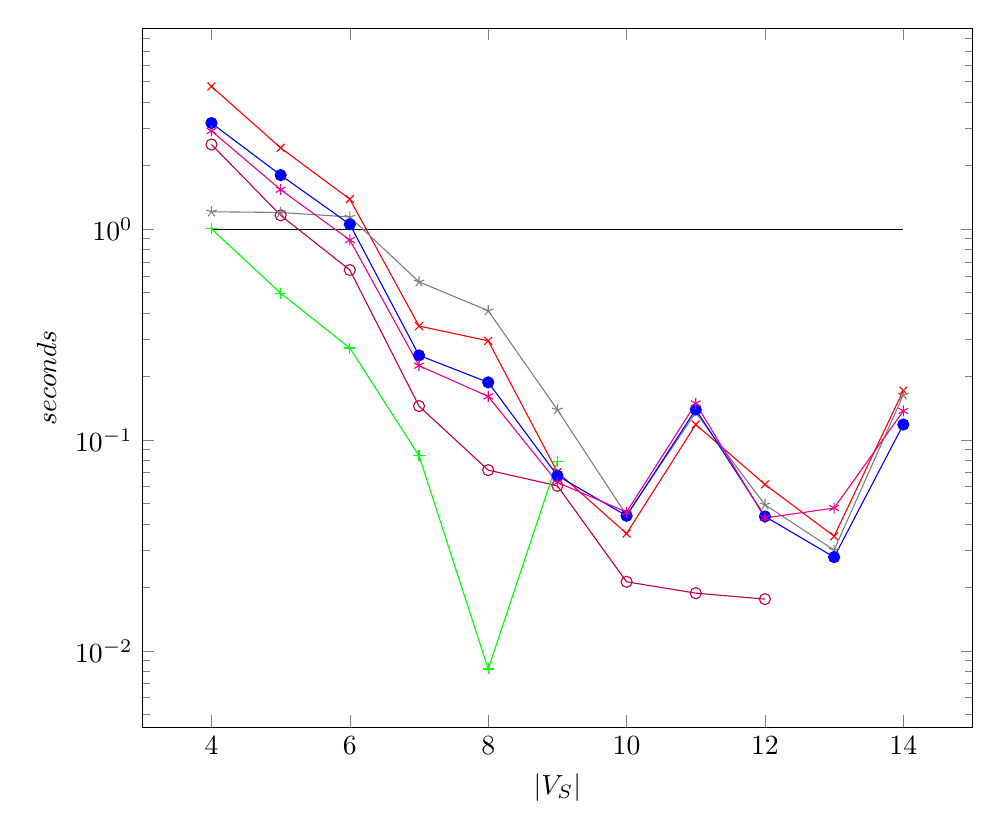
\begin{tikzpicture}
    \begin{axis}[
        xlabel=$|V_S|$,
        ylabel=$seconds$,
        ymode=log,
        legend style={at={(0.9,0.1)},anchor=south east},
        width=\textwidth,
		y tick label style={/pgf/number format/sci},
    ]
\addplot [mark=none, black] plot coordinates {
        (4,1) (14, 1)};



\addplot[
        mark=x,
        red,
    ] plot coordinates {
        (4,4.748759594123889)
        (5,2.4295540762796515)
        (6,1.3875324748809377)
        (7,0.3470734386774885)
        (8,0.2952023716844192)
        (9,0.0703958686196079)
        (10,0.03598320014357281)
        (11,0.1183808662884438)
        (12,0.06153628532584232)
        (13,0.03494338911404371)
        (14,0.17160278085125824)
};
%    \addlegendentry{DFS}


\addplot[
        mark=o,
        purple,
    ] plot coordinates {
        (4,2.519594921852216)
        (5,1.1621656243183787)
        (6,0.6397718531506256)
        (7,0.14471136627669023)
        (8,0.07193325075024548)
        (9,0.0605941046017171)
        (10,0.021240531171245025)
        (11,0.018767566782790235)
        (12,0.01758393553367299)
};
%    \addlegendentry{GDFS O IP}


\addplot[
        mark=star,
        gray,
    ] plot coordinates {
        (4,1.2087512038670705)
        (5,1.1995330941514946)
        (6,1.1418853789726933)
        (7,0.5621877889562694)
        (8,0.41022833627945976)
        (9,0.13903913868573037)
        (10,0.04393563116464705)
        (11,0.13498526740722694)
        (12,0.049268960174921994)
        (13,0.030051623484468215)
        (14,0.1635365740440703)
};
%    \addlegendentry{GDFS C}


\addplot[
        mark=*,
        blue,
    ] plot coordinates {
        (4,3.1851467361084174)
        (5,1.8038765225341042)
        (6,1.0539452554077893)
        (7,0.2518608123839957)
        (8,0.18755266523230274)
        (9,0.06769612412018444)
        (10,0.043697519958703857)
        (11,0.1394520374224132)
        (12,0.04337870481595418)
        (13,0.02780400571582131)
        (14,0.11833494711833015)
};
%    \addlegendentry{K-Path}


\addplot[
        mark=+,
        green,
    ] plot coordinates {
        (4,1.0029463243603973)
        (5,0.49661067861132135)
        (6,0.27286554408201)
        (7,0.08419120306502847)
        (8,0.008199948214019814)
        (9,0.07911018316730134)
};
%    \addlegendentry{CP}


\addplot[
        mark=asterisk,
        magenta,
    ] plot coordinates {
        (4,2.92253226917892)
        (5,1.5385463516143498)
        (6,0.8879009793117698)
        (7,0.22506649596273964)
        (8,0.1609402158565465)
        (9,0.06290335332168706)
        (10,0.04548679530232991)
        (11,0.14892017614069342)
        (12,0.04266555665061478)
        (13,0.04753845861304018)
        (14,0.13727172289974587)
};
%    \addlegendentry{GDFS A IP}

	
    \end{axis}
    \end{tikzpicture}

\caption{parallel}
\label{fig:sub3}
\end{subfigure}
\begin{subfigure} {0.5\linewidth}
\centering

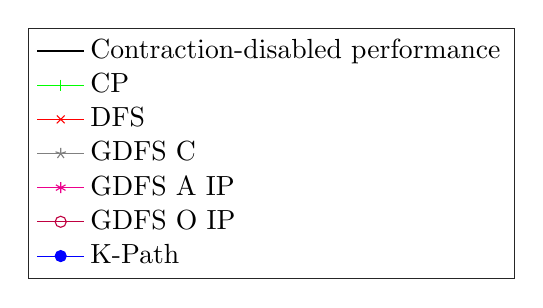
\begin{tikzpicture} 
    \begin{axis}[%
    hide axis,
    xmin=10,
    xmax=50,
    ymin=0,
    ymax=0.4,
    legend style={draw=white!15!black,legend cell align=left}
    ]
	\addlegendimage{black}
    \addlegendentry{Contraction-disabled performance}; 
     
    \addlegendimage{green, mark=+}
    \addlegendentry{CP};
    
    \addlegendimage{red, mark=x}
    \addlegendentry{DFS};
    
    \addlegendimage{gray, mark=star}
    \addlegendentry{GDFS C};
    
    \addlegendimage{magenta, mark=asterisk}
    \addlegendentry{GDFS A IP};
    
    \addlegendimage{purple, mark=o}
    \addlegendentry{GDFS O IP};
    
    \addlegendimage{blue, mark=*}
    \addlegendentry{K-Path};
    
    \end{axis}
\end{tikzpicture}

\end{subfigure}

\caption{Performance of our algorithm with \textbf{AllDifferent} pruning using \textbf{`Free neighbours'} filtering relative to the performance of the algorithm without pruning. We avoid unnecessarily long paths, do not perform contraction and use the degree-based target graph vertex ordering. Data points above the black reference line denote that the pruning method introduces more delay, and data points below the reference line denote that the pruning method saves time. Note the logarithmic y-axis.}		
\label{fig:test}
\end{figure}

\begin{figure}
\begin{subfigure}{.5\linewidth}
\centering

\begin{tikzpicture}
    \begin{axis}[
        xlabel=$|V_S|$,
        ylabel=$seconds$,
        ymode=log,
        legend style={at={(0.9,0.1)},anchor=south east},
        width=\textwidth,
		y tick label style={/pgf/number format/sci},
    ]
\addplot [mark=none, black] plot coordinates {
        (4,1) (14, 1)};


\addplot[
        mark=x,
        red,
    ] plot coordinates {
        (4,0.9961858191755759)
        (5,1.0059848034836174)
        (6,1.0015623854405225)
        (7,1.0041850516247017)
        (8,0.992834292174954)
        (9,0.9805831782750661)
        (10,1.0131070860496907)
        (11,0.9820629029946675)
        (12,0.9731684469245409)
        (13,0.9978012338195624)
};
%    \addlegendentry{DFS}


\addplot[
        mark=o,
        purple,
    ] plot coordinates {
        (4,0.9991254113598864)
        (5,1.0006304793357408)
        (6,0.9997389129846505)
        (7,1.0024122661594037)
        (8,0.9960200414287358)
        (9,0.9797204693043249)
        (10,1.006094756978359)
        (11,1.0291250941127874)
        (12,1.016228045334132)
};
%    \addlegendentry{GDFS O IP}


\addplot[
        mark=star,
        gray,
    ] plot coordinates {
        (4,1.0059277991423625)
        (5,0.9907814973218768)
        (6,1.0243229749286393)
        (7,1.020235901218478)
        (8,1.028660392466402)
        (9,0.9992951555916159)
        (10,0.9825124885953094)
        (11,0.9832292458336007)
        (12,1.0260311821681063)
        (13,1.1015279814561096)
        (14,1.0152331060942739)
};
%    \addlegendentry{GDFS C}


\addplot[
        mark=*,
        blue,
    ] plot coordinates {
        (4,1.1428023873341047)
        (5,0.8363144144880936)
        (6,0.3883692600044063)
        (7,0.12306323448284873)
        (8,0.11750735154321501)
        (9,0.05546079701782758)
        (10,0.027198570773209862)
        (11,0.09188685028611088)
        (12,0.029187752530780098)
        (13,0.028763961047358233)
        (14,0.13514762161751237)
};
%    \addlegendentry{K-Path}


\addplot[
        mark=+,
        green,
    ] plot coordinates {
        (4,1.003240741424298)
        (5,1.0007002255334068)
        (6,0.9998134962523451)
        (7,0.9954368842322697)
        (8,0.9901138150986978)
        (9,1.0994301778756659)
};
%    \addlegendentry{CP}


\addplot[
        mark=asterisk,
        magenta,
    ] plot coordinates {
        (4,1.012208101549136)
        (5,1.004540535143729)
        (6,1.006238667112502)
        (7,0.9987787321626621)
        (8,0.9857632446293185)
        (9,1.00045313105658)
        (10,0.9800057859162024)
        (11,1.0071924078562504)
        (12,1.05284665552656)
        (13,1.0473613609958743)
};
%    \addlegendentry{GDFS A IP}

 

    \end{axis}
    \end{tikzpicture}


\caption{serial}
\label{fig:sub1}
\end{subfigure}%
\begin{subfigure}{.5\linewidth}
\centering

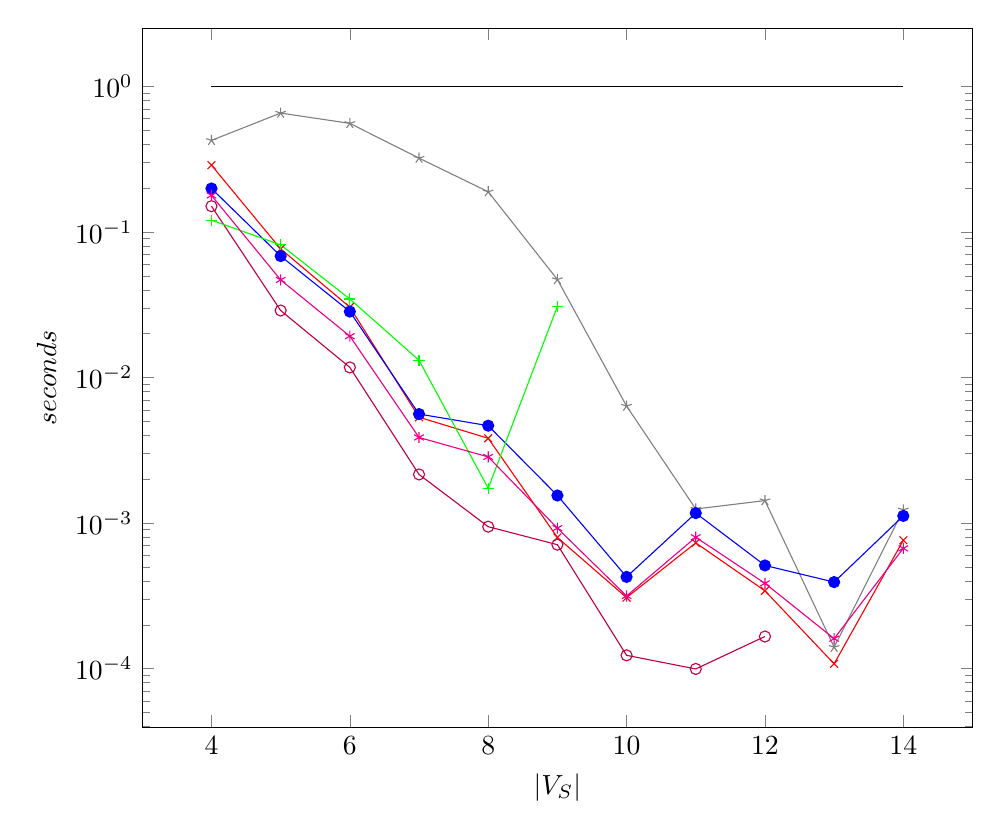
\begin{tikzpicture}
        \begin{axis}[
        xlabel=$|V_S|$,
        ylabel=$seconds$,
        ymode=log,
        legend style={at={(0.9,0.1)},anchor=south east},
        width=\textwidth,
		y tick label style={/pgf/number format/sci},
    ]
\addplot [mark=none, black] plot coordinates {
        (4,1) (14, 1)};

	

\addplot[
        mark=x,
        red,
    ] plot coordinates {
        (4,0.28797946415268216)
        (5,0.07651582579324001)
        (6,0.0304666091954765)
        (7,0.005338589440600172)
        (8,0.0038271200815995776)
        (9,7.967244945263907E-4)
        (10,3.0777658183211987E-4)
        (11,7.316319897914259E-4)
        (12,3.4267518525965546E-4)
        (13,1.0795184070755415E-4)
        (14,7.623451601108666E-4)
};
%    \addlegendentry{DFS}


\addplot[
        mark=o,
        purple,
    ] plot coordinates {
        (4,0.15049515351200515)
        (5,0.028888664846084877)
        (6,0.011744849761370135)
        (7,0.0021597185405343167)
        (8,9.451813259466757E-4)
        (9,7.108005706910614E-4)
        (10,1.2347079460250932E-4)
        (11,9.95681216803268E-5)
        (12,1.6636754548371435E-4)
};
%    \addlegendentry{GDFS O IP}


\addplot[
        mark=star,
        gray,
    ] plot coordinates {
        (4,0.4261569662504955)
        (5,0.6566221486790923)
        (6,0.5577822930842058)
        (7,0.3218592258892897)
        (8,0.18912427965228307)
        (9,0.047186436624101824)
        (10,0.006370129606168451)
        (11,0.0012501421281951863)
        (12,0.001428282896214883)
        (13,1.4047897093971695E-4)
        (14,0.0012339028104273453)
};
%    \addlegendentry{GDFS C}


\addplot[
        mark=*,
        blue,
    ] plot coordinates {
        (4,0.19921889891317368)
        (5,0.06836073093997885)
        (6,0.02840796237713794)
        (7,0.005614455272937469)
        (8,0.004672519202561842)
        (9,0.001547859891521619)
        (10,4.269626026969231E-4)
        (11,0.0011715845435014138)
        (12,5.118613622622226E-4)
        (13,3.9341491023758834E-4)
        (14,0.0011207533086203814)
};
%    \addlegendentry{K-Path}


\addplot[
        mark=+,
        green,
    ] plot coordinates {
        (4,0.12065618974765957)
        (5,0.08159990593923339)
        (6,0.03466025100832615)
        (7,0.013147623578769863)
        (8,0.0017371671223744833)
        (9,0.03084198984204367)
};
%    \addlegendentry{CP}


\addplot[
        mark=asterisk,
        magenta,
    ] plot coordinates {
        (4,0.1784159199448806)
        (5,0.04687838004113365)
        (6,0.019250300262524056)
        (7,0.003877520221788777)
        (8,0.0028497378324052747)
        (9,9.238160016552532E-4)
        (10,3.1576391186238784E-4)
        (11,7.994265736620543E-4)
        (12,3.8594286429616265E-4)
        (13,1.6073739183641855E-4)
        (14,6.707501289580087E-4)
};
%    \addlegendentry{GDFS A IP}

	
    \end{axis}
    \end{tikzpicture}

\caption{cached}
\label{fig:sub2}
\end{subfigure}\\[1ex]
\begin{subfigure}{0.5\linewidth}
\centering

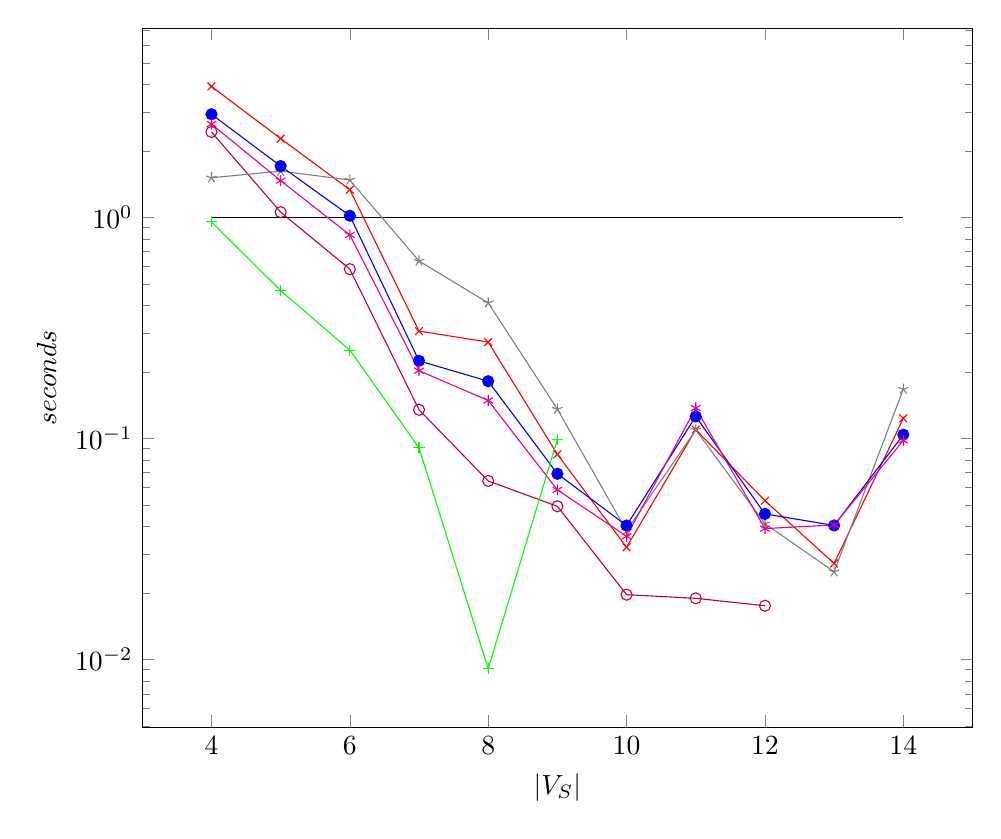
\begin{tikzpicture}
    \begin{axis}[
        xlabel=$|V_S|$,
        ylabel=$seconds$,
        ymode=log,
        legend style={at={(0.9,0.1)},anchor=south east},
        width=\textwidth,
		y tick label style={/pgf/number format/sci},
    ]
\addplot [mark=none, black] plot coordinates {
        (4,1) (14, 1)};


\addplot[
        mark=x,
        red,
    ] plot coordinates {
        (4,3.9129439575545435)
        (5,2.273222753540935)
        (6,1.3358829167973778)
        (7,0.3060292392269831)
        (8,0.27310812493561054)
        (9,0.08483478635788988)
        (10,0.03220002459721227)
        (11,0.10965821877648596)
        (12,0.05238033266084752)
        (13,0.02720606162053374)
        (14,0.12326343330507006)
};
%    \addlegendentry{DFS}


\addplot[
        mark=o,
        purple,
    ] plot coordinates {
        (4,2.4370501012142824)
        (5,1.0568408408459573)
        (6,0.5835598718338068)
        (7,0.13489675395340783)
        (8,0.06428756573066419)
        (9,0.04934951432140211)
        (10,0.01966479503287344)
        (11,0.018929462405664066)
        (12,0.01752267312020006)
};
%    \addlegendentry{GDFS O IP}


\addplot[
        mark=star,
        gray,
    ] plot coordinates {
        (4,1.5119445424232758)
        (5,1.6205884547090093)
        (6,1.4772813435520415)
        (7,0.6353071431015811)
        (8,0.41070975405654797)
        (9,0.13580170759422583)
        (10,0.03828888536206054)
        (11,0.10934140002182946)
        (12,0.0411628308005999)
        (13,0.024956633661657346)
        (14,0.16725255988991872)
};
%    \addlegendentry{GDFS C}


\addplot[
        mark=*,
        blue,
    ] plot coordinates {
        (4,2.9292287176662284)
        (5,1.7085776030673339)
        (6,1.018144876988824)
        (7,0.22453968974110117)
        (8,0.18160614741581238)
        (9,0.06924099256113281)
        (10,0.04038867770933918)
        (11,0.12581531378172073)
        (12,0.04559446907724363)
        (13,0.04043070416472683)
        (14,0.10402774643082491)
};
%    \addlegendentry{K-Path}


\addplot[
        mark=+,
        green,
    ] plot coordinates {
        (4,0.9551312671725737)
        (5,0.46672792929157314)
        (6,0.25108420813909216)
        (7,0.09084564408241347)
        (8,0.009073128728892876)
        (9,0.09911792703918121)
};
%    \addlegendentry{CP}


\addplot[
        mark=asterisk,
        magenta,
    ] plot coordinates {
        (4,2.6450452172441703)
        (5,1.466590988138647)
        (6,0.8335425887125216)
        (7,0.20265590602141004)
        (8,0.14860699155681456)
        (9,0.058559839513090184)
        (10,0.03613722819737897)
        (11,0.1373961637320401)
        (12,0.039138601300597764)
        (13,0.04064207588686031)
        (14,0.09797085693851426)
};
%    \addlegendentry{GDFS A IP}

	
    \end{axis}
    \end{tikzpicture}

\caption{parallel}
\label{fig:sub3}
\end{subfigure}
\begin{subfigure} {0.5\linewidth}
\centering

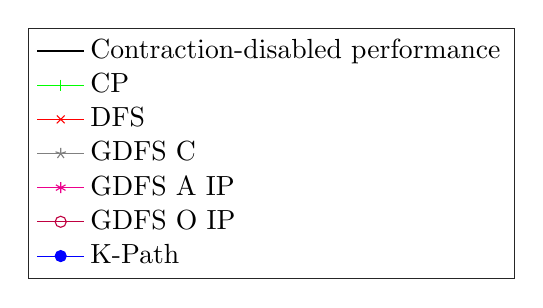
\begin{tikzpicture} 
    \begin{axis}[%
    hide axis,
    xmin=10,
    xmax=50,
    ymin=0,
    ymax=0.4,
    legend style={draw=white!15!black,legend cell align=left}
    ]
	\addlegendimage{black}
    \addlegendentry{Contraction-disabled performance}; 
     
    \addlegendimage{green, mark=+}
    \addlegendentry{CP};
    
    \addlegendimage{red, mark=x}
    \addlegendentry{DFS};
    
    \addlegendimage{gray, mark=star}
    \addlegendentry{GDFS C};
    
    \addlegendimage{magenta, mark=asterisk}
    \addlegendentry{GDFS A IP};
    
    \addlegendimage{purple, mark=o}
    \addlegendentry{GDFS O IP};
    
    \addlegendimage{blue, mark=*}
    \addlegendentry{K-Path};
    
    \end{axis}
\end{tikzpicture}

\end{subfigure}

\caption{Performance of our algorithm with \textbf{AllDifferent} pruning using \textbf{`M-filtering'} filtering relative to the performance of the algorithm without pruning. We avoid unnecessarily long paths, do not perform contraction and use the degree-based target graph vertex ordering. Data points above the black reference line denote that the pruning method introduces more delay, and data points below the reference line denote that the pruning method saves time. Note the logarithmic y-axis.}		
\label{fig:test}
\end{figure}

\begin{figure}
\begin{subfigure}{.5\linewidth}
\centering

\begin{tikzpicture}
    \begin{axis}[
        xlabel=$|V_S|$,
        ylabel=$seconds$,
        ymode=log,
        legend style={at={(0.9,0.1)},anchor=south east},
        width=\textwidth,
		y tick label style={/pgf/number format/sci},
    ]
\addplot [mark=none, black] plot coordinates {
        (4,1) (14,1)};

    
   

\addplot[
        mark=x,
        red,
    ] plot coordinates {
        (4,0.9676950624676575)
        (5,0.9988894067222226)
        (6,1.0005763973495974)
        (7,1.0012522076540606)
        (8,1.0107283953513952)
        (9,0.9599448767629568)
        (10,1.0347901686226628)
        (11,1.0103410684538925)
        (12,1.0255798438058548)
        (13,0.9056614547818025)
        (14,0.9698848854871277)
};
%    \addlegendentry{DFS}


\addplot[
        mark=o,
        purple,
    ] plot coordinates {
        (4,1.0094137822150915)
        (5,1.0030498615384387)
        (6,0.996041126474167)
        (7,1.0014862936237205)
        (8,1.006913278037861)
        (9,0.9865779317721944)
        (10,0.973979329150809)
        (11,1.0085691395261733)
        (12,1.012790208560442)
};
%    \addlegendentry{GDFS O IP}


\addplot[
        mark=star,
        gray,
    ] plot coordinates {
        (4,1.0410716738680912)
        (5,1.008890447711797)
        (6,0.9929773547796908)
        (7,1.0053072922093342)
        (8,1.0058758041034963)
        (9,1.0067325036708086)
        (10,1.0080505476192445)
        (11,0.9598589720985476)
        (12,0.9601497898994072)
        (13,1.05397295806311)
        (14,0.9852887590169078)
};
%    \addlegendentry{GDFS C}


\addplot[
        mark=*,
        blue,
    ] plot coordinates {
        (4,1.5970781583369893)
        (5,1.0429950475098546)
        (6,0.5642557451473594)
        (7,0.19187744681948582)
        (8,0.16271009963035188)
        (9,0.0715045220335021)
        (10,0.046728031478004195)
        (11,0.10603600840907235)
        (12,0.03729878780829776)
        (13,0.04017799631235486)
        (14,0.1473463960242647)
};
%    \addlegendentry{K-Path}


\addplot[
        mark=+,
        green,
    ] plot coordinates {
        (4,1.0136425248501462)
        (5,1.0007246262269673)
        (6,0.9976668304761186)
        (7,0.9885168025956491)
        (8,1.0110440897106538)
        (9,1.0265495887464324)
};
%    \addlegendentry{CP}


\addplot[
        mark=asterisk,
        magenta,
    ] plot coordinates {
        (4,0.9925924238577477)
        (5,0.9932698347961497)
        (6,1.002644406556925)
        (7,1.0082608252132723)
        (8,1.0002625398016867)
        (9,0.9673299243637845)
        (10,1.0357874894276926)
        (11,1.0267563810636593)
        (12,1.015497232110587)
        (13,1.0002726400770723)
};
%    \addlegendentry{GDFS A IP}


    \end{axis}
    \end{tikzpicture}


\caption{serial}
\label{fig:sub1}
\end{subfigure}%
\begin{subfigure}{.5\linewidth}
\centering

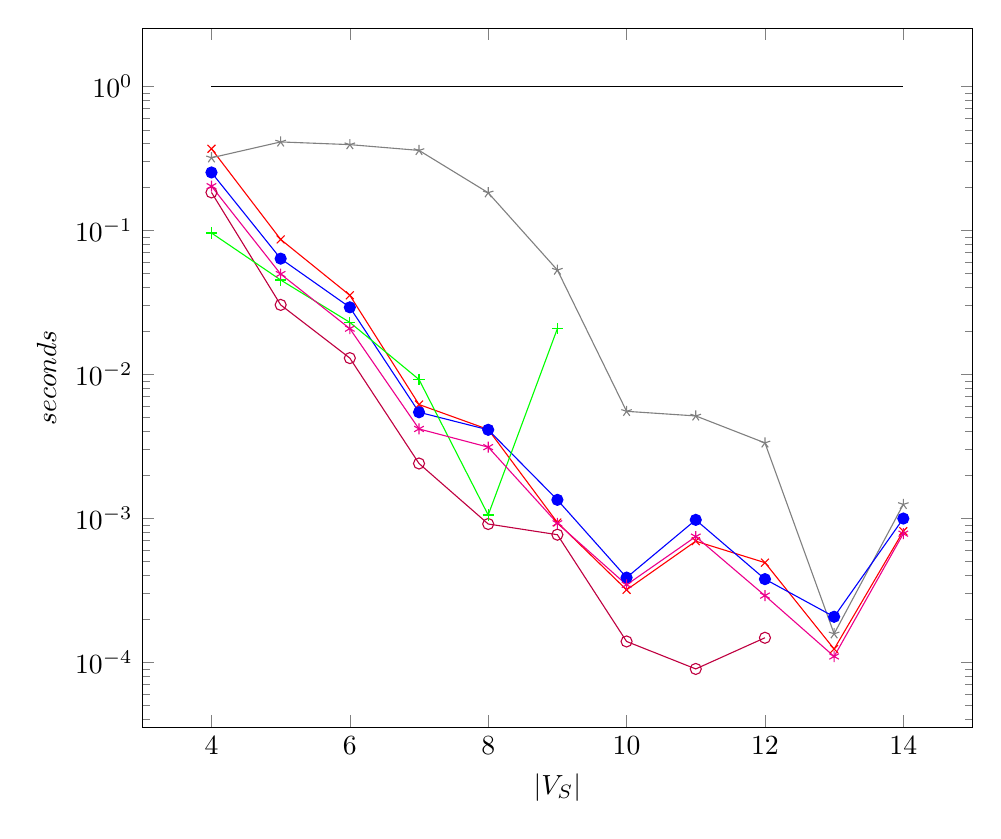
\begin{tikzpicture}
    \begin{axis}[
        xlabel=$|V_S|$,
        ylabel=$seconds$,
        ymode=log,
        legend style={at={(0.9,0.1)},anchor=south east},
        width=\textwidth,
		y tick label style={/pgf/number format/sci},
    ]
\addplot [mark=none, black] plot coordinates {
        (4,1) (14, 1)};


	

\addplot[
        mark=x,
        red,
    ] plot coordinates {
        (4,0.3693236491674021)
        (5,0.08662776836402786)
        (6,0.03543362590095955)
        (7,0.006177208718380012)
        (8,0.004144420637945623)
        (9,9.354448414969907E-4)
        (10,3.1869623984615014E-4)
        (11,6.942032052866809E-4)
        (12,4.92629092351704E-4)
        (13,1.236654683463012E-4)
        (14,8.145275946982444E-4)
};
%    \addlegendentry{DFS}


\addplot[
        mark=o,
        purple,
    ] plot coordinates {
        (4,0.18371858693151044)
        (5,0.030401734904650368)
        (6,0.012976374788824407)
        (7,0.002405059847648494)
        (8,9.138047489324341E-4)
        (9,7.701810544392673E-4)
        (10,1.3963369512837165E-4)
        (11,8.996547626749507E-5)
        (12,1.4807292756369161E-4)
};
%    \addlegendentry{GDFS O IP}


\addplot[
        mark=star,
        gray,
    ] plot coordinates {
        (4,0.3196707718030456)
        (5,0.4119004671239389)
        (6,0.3945929975644642)
        (7,0.3597088103007954)
        (8,0.18276813544122272)
        (9,0.053068079095563214)
        (10,0.005540376398996627)
        (11,0.005146721461176784)
        (12,0.0033440271263982524)
        (13,1.5787860587113123E-4)
        (14,0.0012506224638044738)
};
%    \addlegendentry{GDFS C}


\addplot[
        mark=*,
        blue,
    ] plot coordinates {
        (4,0.25280034627371606)
        (5,0.06370234194664193)
        (6,0.02923362323560863)
        (7,0.005458665126135687)
        (8,0.004121676516919193)
        (9,0.0013445510878975497)
        (10,3.8782765857092727E-4)
        (11,9.762077809364333E-4)
        (12,3.7839915244086697E-4)
        (13,2.0719974514915585E-4)
        (14,9.972179281756421E-4)
};
%    \addlegendentry{K-Path}


\addplot[
        mark=+,
        green,
    ] plot coordinates {
        (4,0.09603666224543228)
        (5,0.045282268345635424)
        (6,0.022983591743019782)
        (7,0.009213437075401898)
        (8,0.0010550572324501406)
        (9,0.020807435412101838)
};
%    \addlegendentry{CP}


\addplot[
        mark=asterisk,
        magenta,
    ] plot coordinates {
        (4,0.20290440891034733)
        (5,0.04978550630960299)
        (6,0.020792134867174017)
        (7,0.004179165900801252)
        (8,0.0031241683734722914)
        (9,9.241937127778543E-4)
        (10,3.455504261065112E-4)
        (11,7.470512282303776E-4)
        (12,2.9066662540455646E-4)
        (13,1.0982181047392015E-4)
        (14,7.830472075457395E-4)
};
%    \addlegendentry{GDFS A IP}

	
    \end{axis}
    \end{tikzpicture}

\caption{cached}
\label{fig:sub2}
\end{subfigure}\\[1ex]
\begin{subfigure}{0.5\linewidth}
\centering

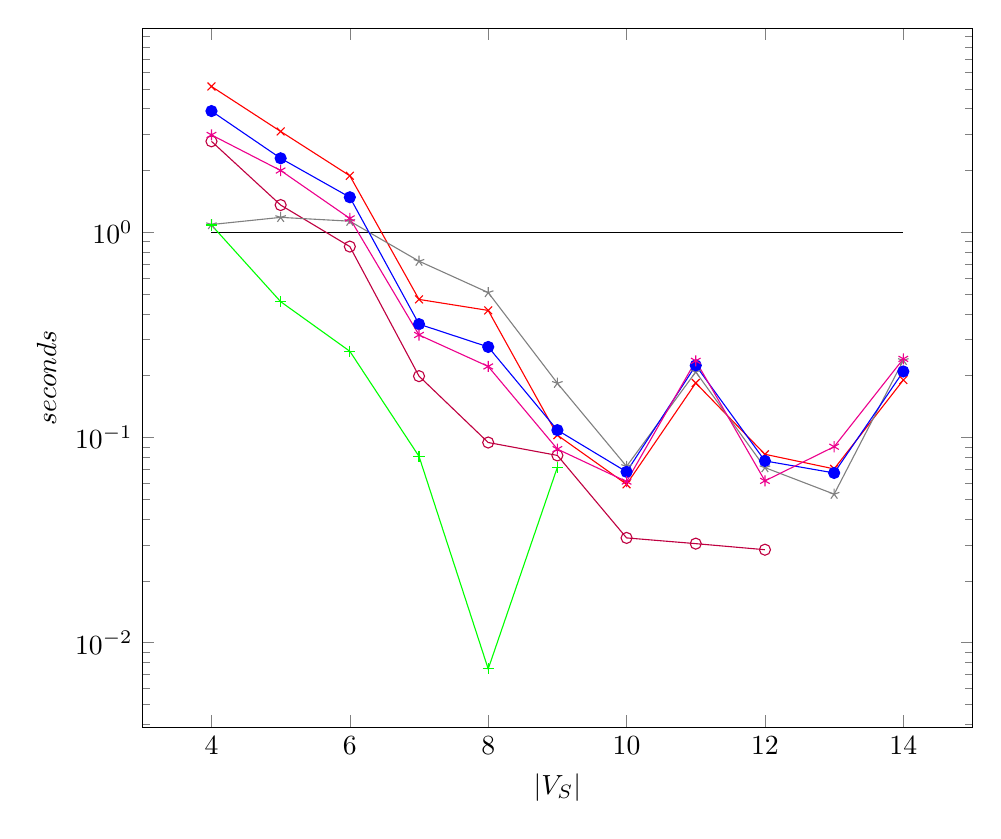
\begin{tikzpicture}
    \begin{axis}[
        xlabel=$|V_S|$,
        ylabel=$seconds$,
        ymode=log,
        legend style={at={(0.9,0.1)},anchor=south east},
        width=\textwidth,
		y tick label style={/pgf/number format/sci},
    ]
\addplot [mark=none, black] plot coordinates {
        (4,1) (14, 1)};



\addplot[
        mark=x,
        red,
    ] plot coordinates {
        (4,5.1345832619134315)
        (5,3.100425102383263)
        (6,1.8852096728253702)
        (7,0.4708800143588947)
        (8,0.41618998589925804)
        (9,0.1027206607222183)
        (10,0.059163250604911566)
        (11,0.18439902177485434)
        (12,0.08285693958613916)
        (13,0.07033185960559696)
        (14,0.19062567426078747)
};
%    \addlegendentry{DFS}


\addplot[
        mark=o,
        purple,
    ] plot coordinates {
        (4,2.774994132451617)
        (5,1.3574173398460796)
        (6,0.851912409726081)
        (7,0.1991114927169909)
        (8,0.09455509094612868)
        (9,0.0818077201557178)
        (10,0.03242406032574496)
        (11,0.03040410201940047)
        (12,0.028403050719100542)
};
%    \addlegendentry{GDFS O IP}


\addplot[
        mark=star,
        gray,
    ] plot coordinates {
        (4,1.0909185494014733)
        (5,1.182187346908493)
        (6,1.1328378765879803)
        (7,0.7233308955429363)
        (8,0.5086224425944339)
        (9,0.18394420655553456)
        (10,0.07234125105236022)
        (11,0.20874358974197005)
        (12,0.07136307095042382)
        (13,0.05297957121058816)
        (14,0.23772304496314955)
};
%    \addlegendentry{GDFS C}


\addplot[
        mark=*,
        blue,
    ] plot coordinates {
        (4,3.8970195420742755)
        (5,2.2939604690071147)
        (6,1.481691252343444)
        (7,0.35686658381717284)
        (8,0.2762673233671855)
        (9,0.10864296003618246)
        (10,0.06803550925927393)
        (11,0.22460191218117787)
        (12,0.07692161844416523)
        (13,0.06719809667315302)
        (14,0.20985511070050933)
};
%    \addlegendentry{K-Path}


\addplot[
        mark=+,
        green,
    ] plot coordinates {
        (4,1.0848428708890463)
        (5,0.4591837362904758)
        (6,0.26321451914524563)
        (7,0.0809303914306656)
        (8,0.007455460280270221)
        (9,0.07164052373260954)
};
%    \addlegendentry{CP}


\addplot[
        mark=asterisk,
        magenta,
    ] plot coordinates {
        (4,2.981403961199849)
        (5,2.00009795935702)
        (6,1.168640642979861)
        (7,0.31603922204888457)
        (8,0.22195394127915336)
        (9,0.08780473818064749)
        (10,0.06100100883433479)
        (11,0.23639828072837477)
        (12,0.06149452415020673)
        (13,0.09018840369746495)
        (14,0.24168554995385316)
};
%    \addlegendentry{GDFS A IP}

	
    \end{axis}
    \end{tikzpicture}

\caption{parallel}
\label{fig:sub3}
\end{subfigure}
\begin{subfigure} {0.5\linewidth}
\centering

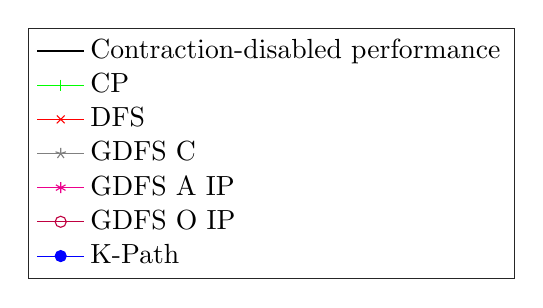
\begin{tikzpicture} 
    \begin{axis}[%
    hide axis,
    xmin=10,
    xmax=50,
    ymin=0,
    ymax=0.4,
    legend style={draw=white!15!black,legend cell align=left}
    ]
	\addlegendimage{black}
    \addlegendentry{Contraction-disabled performance}; 
     
    \addlegendimage{green, mark=+}
    \addlegendentry{CP};
    
    \addlegendimage{red, mark=x}
    \addlegendentry{DFS};
    
    \addlegendimage{gray, mark=star}
    \addlegendentry{GDFS C};
    
    \addlegendimage{magenta, mark=asterisk}
    \addlegendentry{GDFS A IP};
    
    \addlegendimage{purple, mark=o}
    \addlegendentry{GDFS O IP};
    
    \addlegendimage{blue, mark=*}
    \addlegendentry{K-Path};
    
    \end{axis}
\end{tikzpicture}

\end{subfigure}

\caption{Performance of our algorithm with \textbf{AllDifferent} pruning using \textbf{`N-filtering'} filtering relative to the performance of the algorithm without pruning. We avoid unnecessarily long paths, do not perform contraction and use the degree-based target graph vertex ordering. Data points above the black reference line denote that the pruning method introduces more delay, and data points below the reference line denote that the pruning method saves time. Note the logarithmic y-axis.}		
\label{fig:test}
\end{figure}


%cached zero domain (no labels) times \ref{fig:contractionsmall} timeout 30m
\begin{figure}
\centering
\begin{tikzpicture}
    \begin{axis}[
        xlabel=$|V_S|$,
        ylabel=$seconds$,
        ymin=-100,
        ymax=100,
        xmin=4,
        xmax=18.5,
        legend style={at={(0.9,0.1)},anchor=south east},
        width=\textwidth,
        yticklabel={$\pgfmathprintnumber{\tick}\%$},
    ]

\addplot [mark=none, black] plot coordinates {
        (4,0) (18.5, 0)};
\addlegendentry{No contraction}



    \end{axis}
    \end{tikzpicture}
    \caption{Relative time consumption of contraction-enabled subgraph homeomorphism search compared to contraction-disabled for different path iteration methods.}
    \label{fig:contractionsmall}
\end{figure}


